% WRF4DVar LBC
% March 2010 
% Autor: Xin Zhang 
% MMM, National Center for Atmospheric Research
% www.mmm.ucar.edu
% email: xinzhang@ucar.edu

\documentclass[handout]{beamer}
\usepackage{pgfpages}
%\pgfpagesuselayout{4 on 1}[a4paper, landscape,border shrink=10mm]
%\mode<handout>{\setbeamercolor{background canvas}{bg=black!5}}
\usepackage{amsmath,amssymb}
%\usepackage{times}
%\usefonttheme{serif} 
\setbeamercovered{dynamic}
\setbeamertemplate{navigation symbols}{}
\usepackage[english]{babel}
\usetheme{Warsaw}
\usecolortheme{rose} 
\usepackage{graphicx}
\usepackage{hyperref}
\usepackage{comment}
\beamersetuncovermixins{\opaqueness<1>{25}}{\opaqueness<2->{15}}
\begin{document}

\title[LBC control in WRF 4D-Var]{Lateral Boundary Condition (LBC) Control \\in WRF 4D-Var System}

\author[Xin Zhang et al.]{Xin Zhang\inst{1} \and Hans Huang\inst{1} \and Nils Gustafsson\inst{2}}
\institute[NCAR]{\inst{1} National Center for Atmospheric Research, Boulder, CO USA \and \inst{2} Swedish Meteorological and Hydrological Institute, Norrkoping, Sweden}
\date{The 9th Workshop on Adjoint Model Applications, Sicily, Italy}
\logo{
\includegraphics[scale=0.05]{NSF_NESL}}


\frame{\titlepage}

\begin{frame}
\frametitle{Outline} 
\tableofcontents
\end{frame}

\section{Motivation}
\begin{frame}
\frametitle{Why is LBC Control  needed  for \color{red}Regional 4D-Var?}
\begin{itemize}
\item The Limited Area Model  forecasting is a Lateral Boundary Condition (LBC) problem + Initial Condition (IC) problem \pause
\item Errico and Vukicevic (1993) show that the forecast error sensitivity with respect to a LBC field might has greater magnitude than for a corresponding IC field in a winter case with MM4 adjoint model.\pause
\item Gustafsson and Kallen (1998) indicate that errors in IC as well as in LBC may explain some forecast failures \dots .
\end{itemize}
\end{frame}

\begin{frame}
\frametitle{Why is LBC Control  needed  for \color{red}Regional 4D-Var?}
\begin{itemize}
\item Phenomena that are observed inside the domain during the later part of the 4D-Var data assimilation window may influence the initial conditions, while being propagated by backward adjoint integration through the lateral boundaries during the early part of the data assimilation window \pause
\item Those observed information related to these phenomena may be lost if LBC are not controlled.
\end{itemize}
\end{frame}

\section{WRF 4D-Var LBC Control}

\subsection{WRF 4D-Var formulation}

\begin{frame}
\frametitle{WRF 4D-Var cost function}
\begin{itemize}
	\item Total cost function: \\ $J=J_b+J_o+J_c$ 
	\vspace{2mm}
	\pause
	\item Background term: \\ 
			$J_{b}=\frac{1}{2}(\mathbf{x}(t_0)-\mathbf{x}_b)^T\mathbf{B}^{-1}(\mathbf{x}(t_0)-\mathbf{x}_b)$
	\vspace{2mm}
	\pause
	\item Observational term: \\
			$J_{o}=\frac{1}{2}\sum_{k=0}^K (H(\mathbf{x}(t_k))-\mathbf{y}^o(t_k))^T\mathbf{O}^{-1}(H(\mathbf{x}(t_k))-\mathbf{y}^o(t_k))$
	\vspace{2mm}
	\pause
	\item $J_c$ is the balance term: digital filter
\end{itemize}
\end{frame}

\begin{frame}
\frametitle{WRF 4D-Var cost function \color{red}with LBC control}
\begin{itemize}
	\item Total cost function: \\ $J=J_b+J_o+J_c+{\color{red}J_{lbc}}$
	\vspace{2mm}
	\pause
	\item How to define LBC term? \\
		$J_{lbc} = \frac{1}{2}(?-?)^T\mathbf{?}^{-1}(?-?)$ 
\end{itemize}
\end{frame}

\subsection{WRF specified boundary condition}
\begin{frame}
\frametitle{WRF specified boundary condition}
\center{
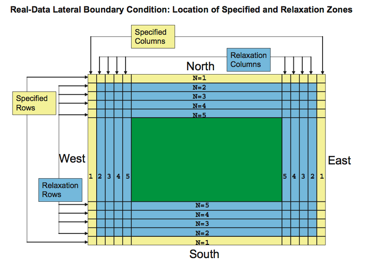
\includegraphics[scale=0.4]{wrfLbc}
}
\begin{itemize}
\item WRF lateral boundary : {\color{yellow}Specified zone} +{\color{blue} Relaxation zone} \pause
\item {\color{yellow}Specified zone} : temporal interpolation from an external forecast or analysis \pause
\item {\color{blue}Relaxation zone} : where the model is nudged or relaxed towards the large-scale forecast
\end{itemize}
\end{frame}
   
\begin{frame}
\frametitle{Relaxation zone}
\begin{itemize}
\item Following Davies and Turner (1977):
\begin{equation*}
\frac{\partial{\mathbf{x}}}{\partial{t}}=F_1(\mathbf{x}_{lbc}-\mathbf{x}) - F_2\Delta^2(\mathbf{x}_{lbc}-\mathbf{x})
\end{equation*} 
where $\Delta^2$ is a 5-point smoothing operator,$ F_1$ and $F_2$ are (nudging) 
weighting coefficients depending on the distance to the lateral boundary \pause
\item  $\mathbf{x}_{lbc}$ is the corresponding boundary value provided by the host model, which
is speci�ed in the following form:
\begin{equation*}
\mathbf{x}_{lbc}(t)=\mathbf{x}_{lbc}(t_0)+(t-t_0)\frac{\partial{\mathbf{x}_{lbc}}}{\partial{t}}
\end{equation*}
\end{itemize}
\end{frame}

\begin{frame}
\frametitle{WRF LBC}
WRF LBC has two parts: 
\begin{itemize}
\item The starting values of variables within the outer most rows and columns $\mathbf{x}_{lbc}(t_0)$.
\item  The tendency of variables within the outer most rows and columns $\frac{\partial{\mathbf{x}_{lbc}}}{\partial{t}}$, assume the LBC update interval is from $t_0$ to $t_k$
\begin{equation*}
\frac{\partial{\mathbf{x}_{lbc}}}{\partial{t}}=\frac{\mathbf{x}_{lbc}(t_k) - \mathbf{x}_{lbc}(t_0)}{t_k-t_0}
\end{equation*} 
\end{itemize}
$\mathbf{x}_{lbc}(t_0)$ is extracted from the first guess $\mathbf{x}_b$ \\
$\mathbf{x}_{lbc}(t_k)$ is extracted from the first guess $\mathbf{x}_b$ at $t_k$
\end{frame}

\begin{frame}
\frametitle{WRF LBC control}
\begin{itemize}
\item In WRF 4D-Var, if the LBC update interval $t_k$ is equal to the assimilation window (mandatory in practice), the LBC control problem can be reduced to control the model states at both the start and the end of the assimilation window.
\item Since it is difficult to only control the model states within the outer most few rows and columns, the whole fields at the end of the assimilation window will be controlled.
\end{itemize}
\end{frame}

\begin{frame}
\frametitle{WRF LBC control -- first guess}
\begin{figure} 
\centering 
\centering 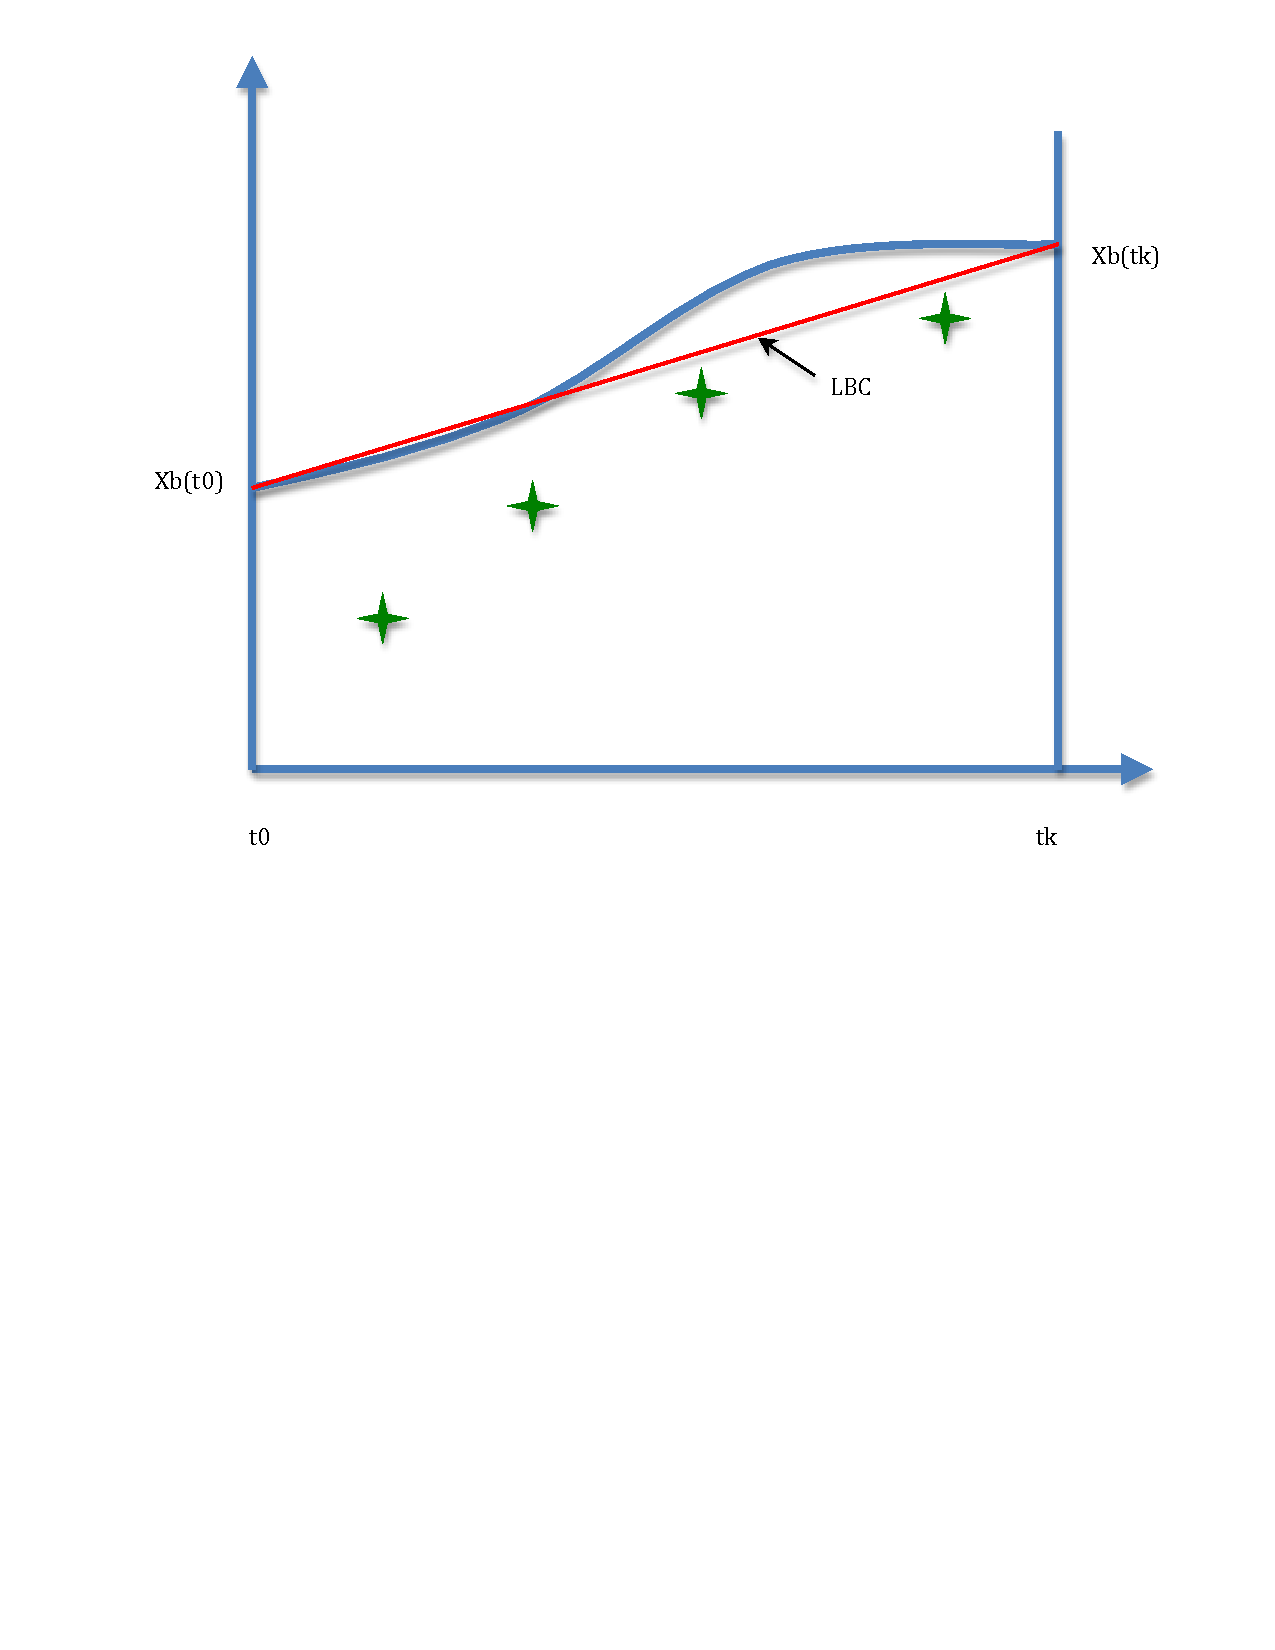
\includegraphics[trim=40 230 40 10, clip=true, width=0.7\textwidth]{figures/wo_lbc_0} 
\end{figure} 
\end{frame}

\begin{frame}
\frametitle{WRF LBC control -- without LBC control}
\begin{figure} 
\centering 
\centering 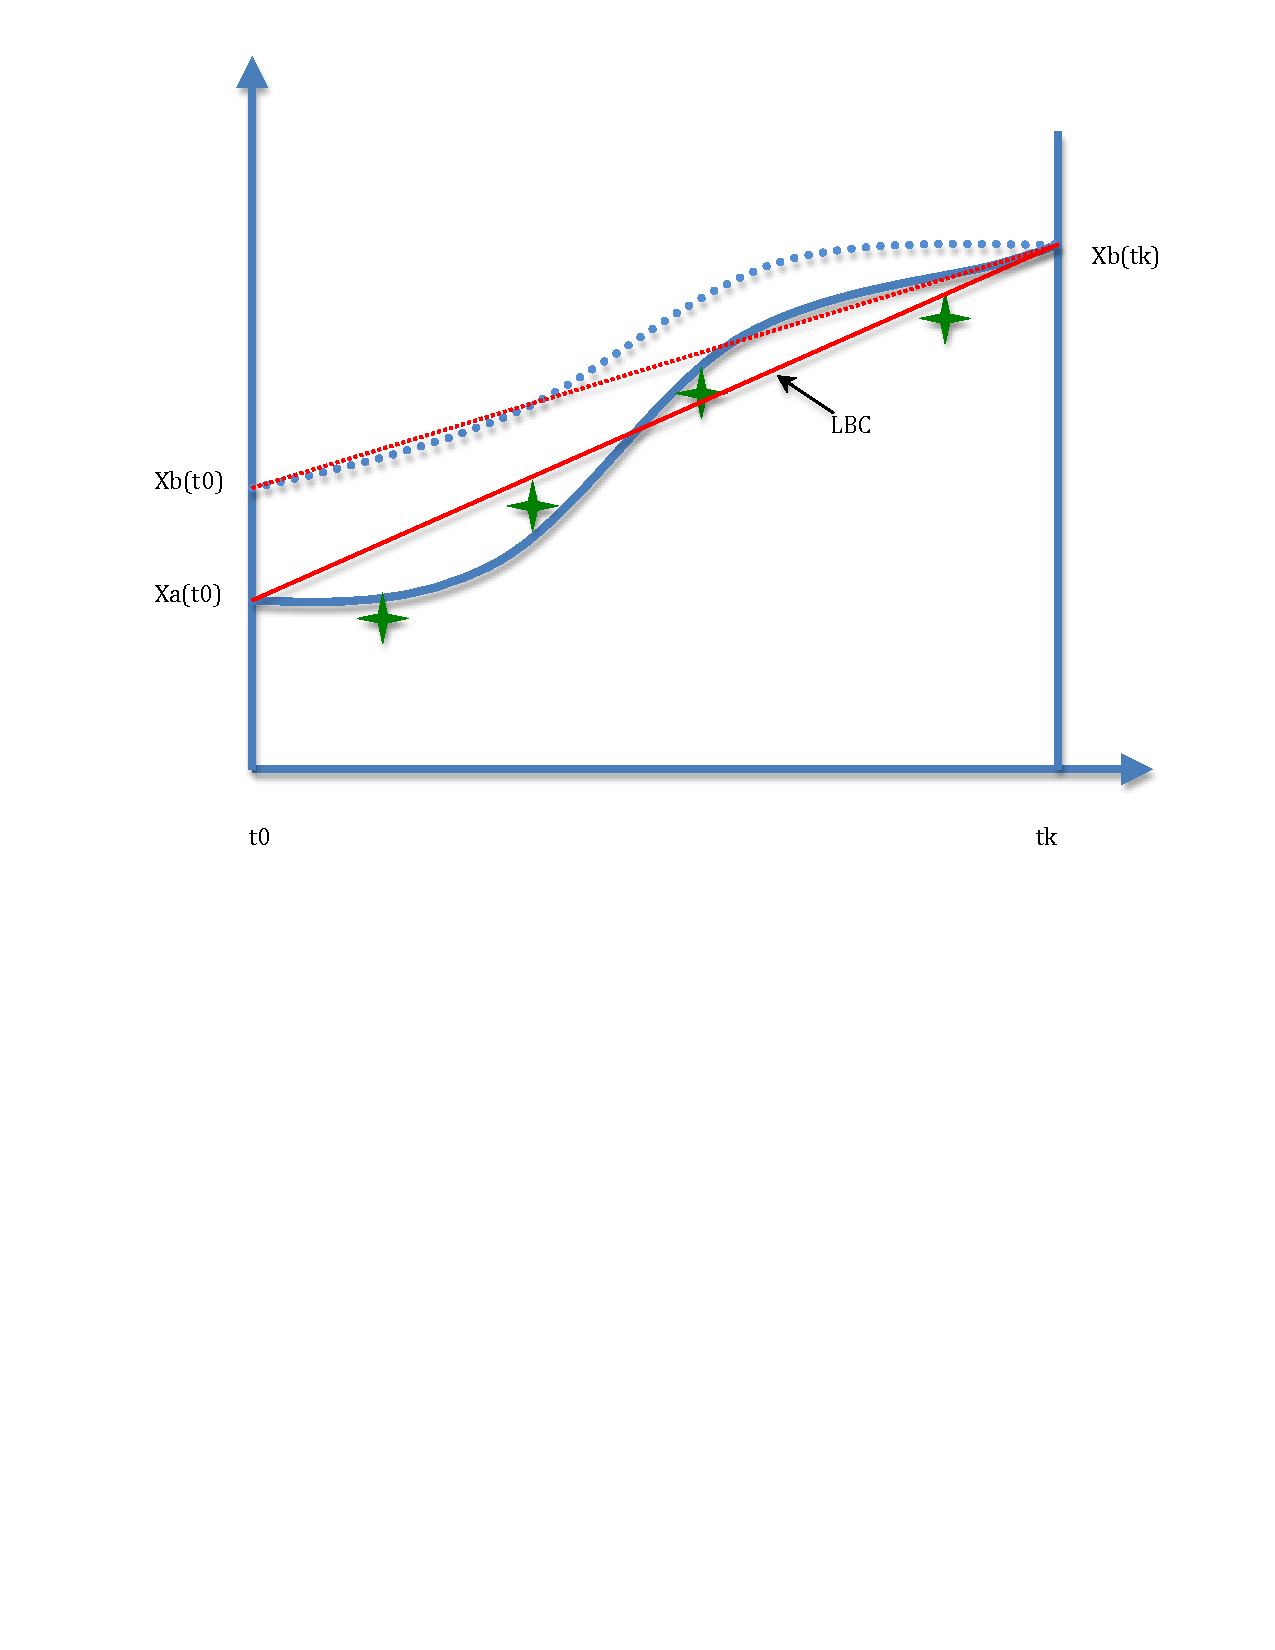
\includegraphics[trim=40 230 40 10, clip=true, width=0.7\textwidth]{figures/wo_lbc_1} 
\end{figure} 
\end{frame}

\begin{frame}
\frametitle{WRF LBC control -- with LBC control}
\begin{figure} 
\centering 
\centering 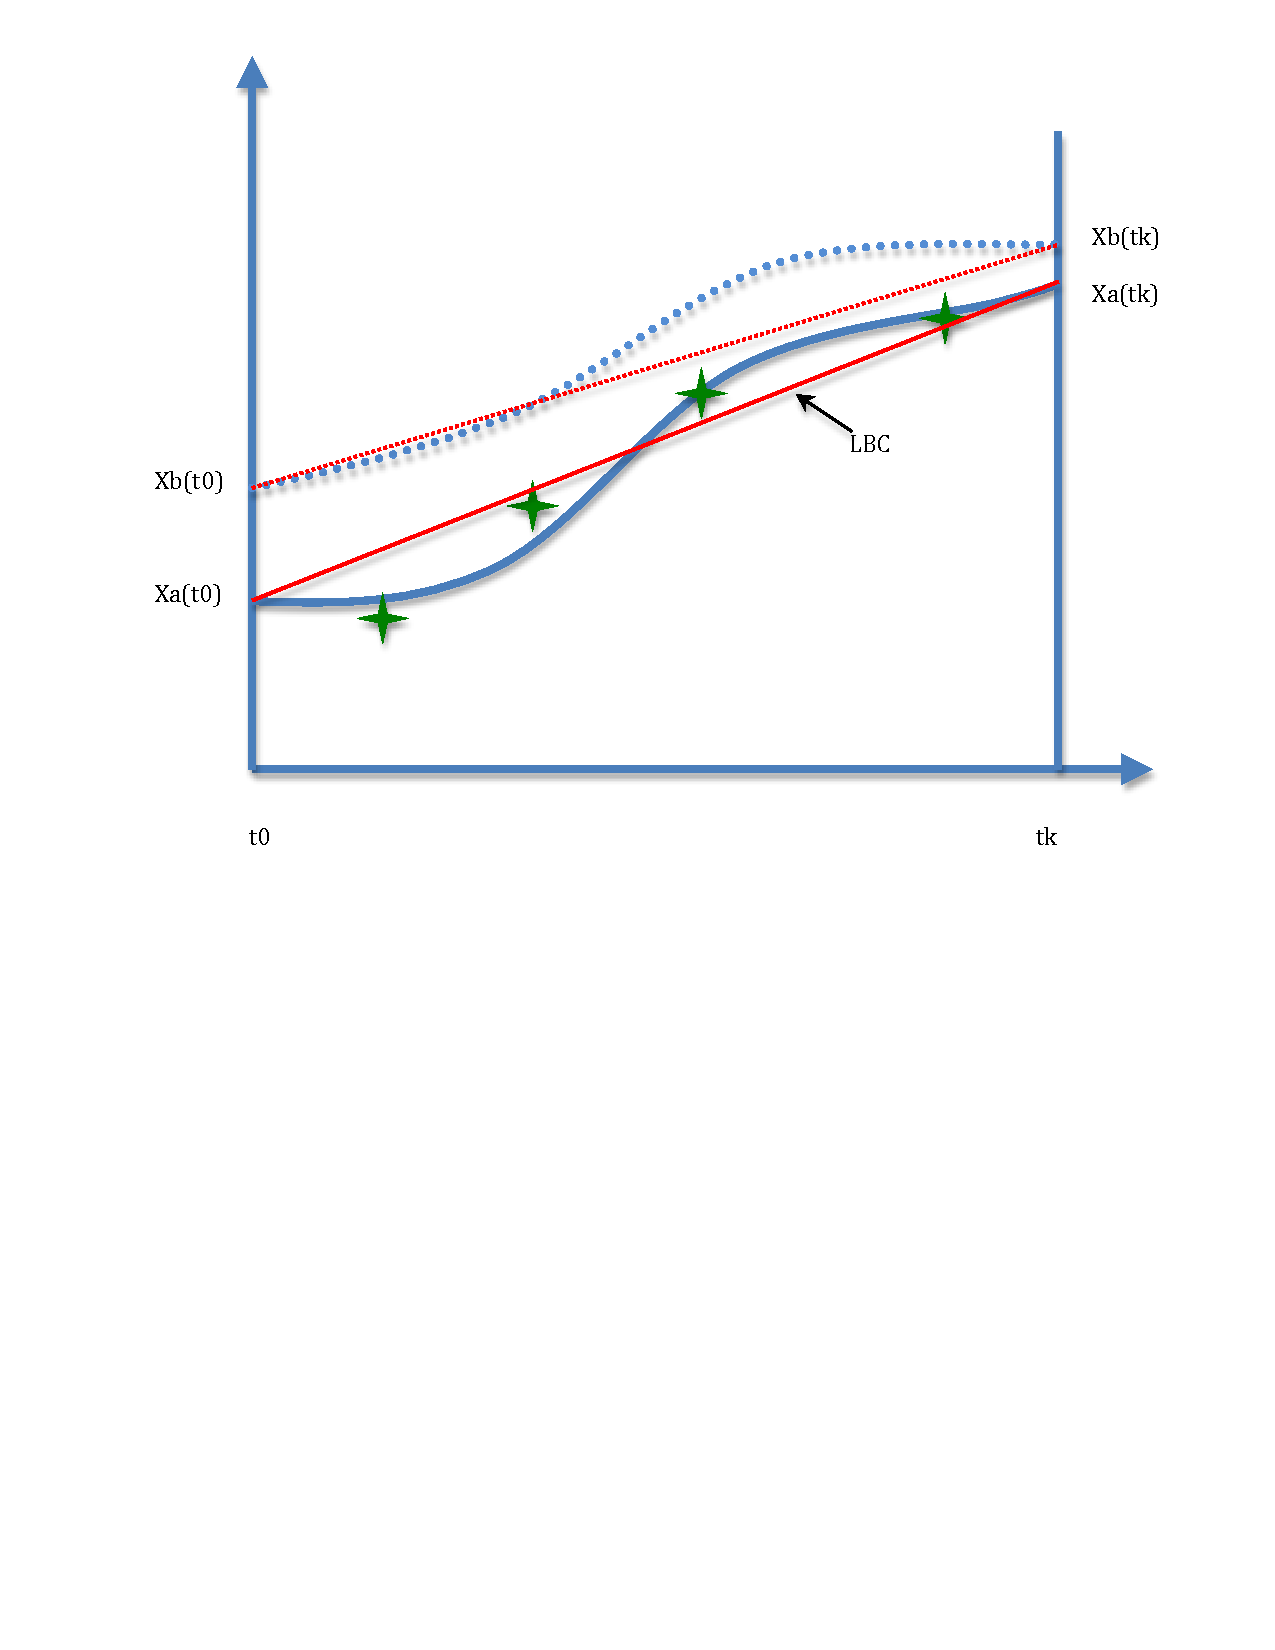
\includegraphics[trim=40 230 40 10, clip=true, width=0.7\textwidth]{figures/w_lbc_1} 
\end{figure} 
\end{frame}

\subsection {4D-Var with LBC control implementation}

\begin{frame}
\frametitle{4D-Var with LBC Control Implementation}
Following Kawabata et al. (2007), under context of incremental variational formulation, considering a data assimilation window from time $t_0$ until time $t_k$ and having $\delta{\mathbf{x}}(t_0)$ and $\delta{\mathbf{x}_{lbc}}(t_k)$ as the assimilation control variables
\begin{equation*}
J=J_b+J_o+J_c+\color{red}J_{lbc}
\end{equation*}
\begin{eqnarray*}
J_{lbc} & = & \frac{1}{2}(\mathbf{x}(t_k)-\mathbf{x}_b(t_k))^T\mathbf{B}^{-1}(\mathbf{x}(t_k)-\mathbf{x}_b(t_k))\\
& = & \frac{1}{2}\delta\mathbf{x}(t_k)^T\mathbf{B}^{-1}\delta\mathbf{x}({t_k})
\end{eqnarray*}
$J_{lbc}$ is the $J_b$ at the end of the assimilation window \\
lateral boundary control is obtained through
\begin{eqnarray*}
\frac {\partial{\delta{\mathbf{x}}_{lbc}}} {\partial{t}}=\frac{\delta\mathbf{x}(t_k)-\delta\mathbf{x}(t_0)}{t_k-t_0}
\end{eqnarray*}
\end{frame}

\begin{frame}
\frametitle{LBC perturbation}
The quantities needed for the LBC of the tangent linear model are given by
\begin{equation*}
\delta{\mathbf{x}}_{lbc}(t_0)=\delta{\mathbf{x}}(t_0)
\end{equation*}
\begin{equation*}
\frac {\partial{\delta{\mathbf{x}}_{lbc}}} {\partial{t}}=\frac{\delta{\mathbf{x}}_{lbc}(t_k)-\delta{\mathbf{x}}(t_0)} {t_k-t_0}
\end{equation*}
\end{frame}

\begin{frame}
\frametitle{LBC adjoint}
The LBC for the adjoint model, $\mathbf{x}_{lbc}^{AD}$ and $(\frac{\partial{\mathbf{x}}_{lbc}} {\partial{t}})^{AD}$
, will be initialized with zeroes at the end of the data assimilation 
window (time $t_k$). After the backwards integration of the adjoint model to 
time $t_0$, the adjoint control variables (or the gradients) can be obtained 
from: 
\begin{equation*}
\mathbf{x}_{ic}^{AD}(t_0)=\mathbf{x}_{ic}^{AD}(t_0)+\mathbf{x}_{lbc}^{AD}(t_0)-\frac{1}{t_k-t_0}(\frac{\partial{\mathbf{x}_{lbc}}}{\partial{t}})^{AD}
\end{equation*}
\begin{equation*}
\mathbf{x}_{lbc}^{AD}(t_k)=\frac{1}{t_k-t_0}(\frac{\partial{\mathbf{x}_{lbc}}}{\partial{t}})^{AD}
\end{equation*}
where $\mathbf{x}_{ic}^{AD}(t_0)$ denotes the �inner domain� adjoint model model variable as provided at the initial time $t_0$.
\end{frame}

\section{Single Observation Experiments}

\begin{frame}
\begin{itemize}
\item Analysis increments due to a single observation produced by a 4D-Var system describe how the tangent linear and adjoint model propagate the observational information.
\item Putting a simulated 500hPa temperature observation at 6h (at the end of the assimilation window) close to inflow lateral boundary (within relaxation zone), we expect some information will be propagated from the inflow lateral boundary.
\end{itemize}
\end{frame}

\begin{comment}
\subsection{ A 6 h observation away from boundary ($\Delta T= 2K$)}

\begin{frame}
\frametitle{500hPa $\theta$ analysis increments at 0 h}
$\color{red}\textbf{+}$ is the location of the observation at 6h
\begin{columns}[T]
	\begin{column}{6cm}
		\begin{figure}
			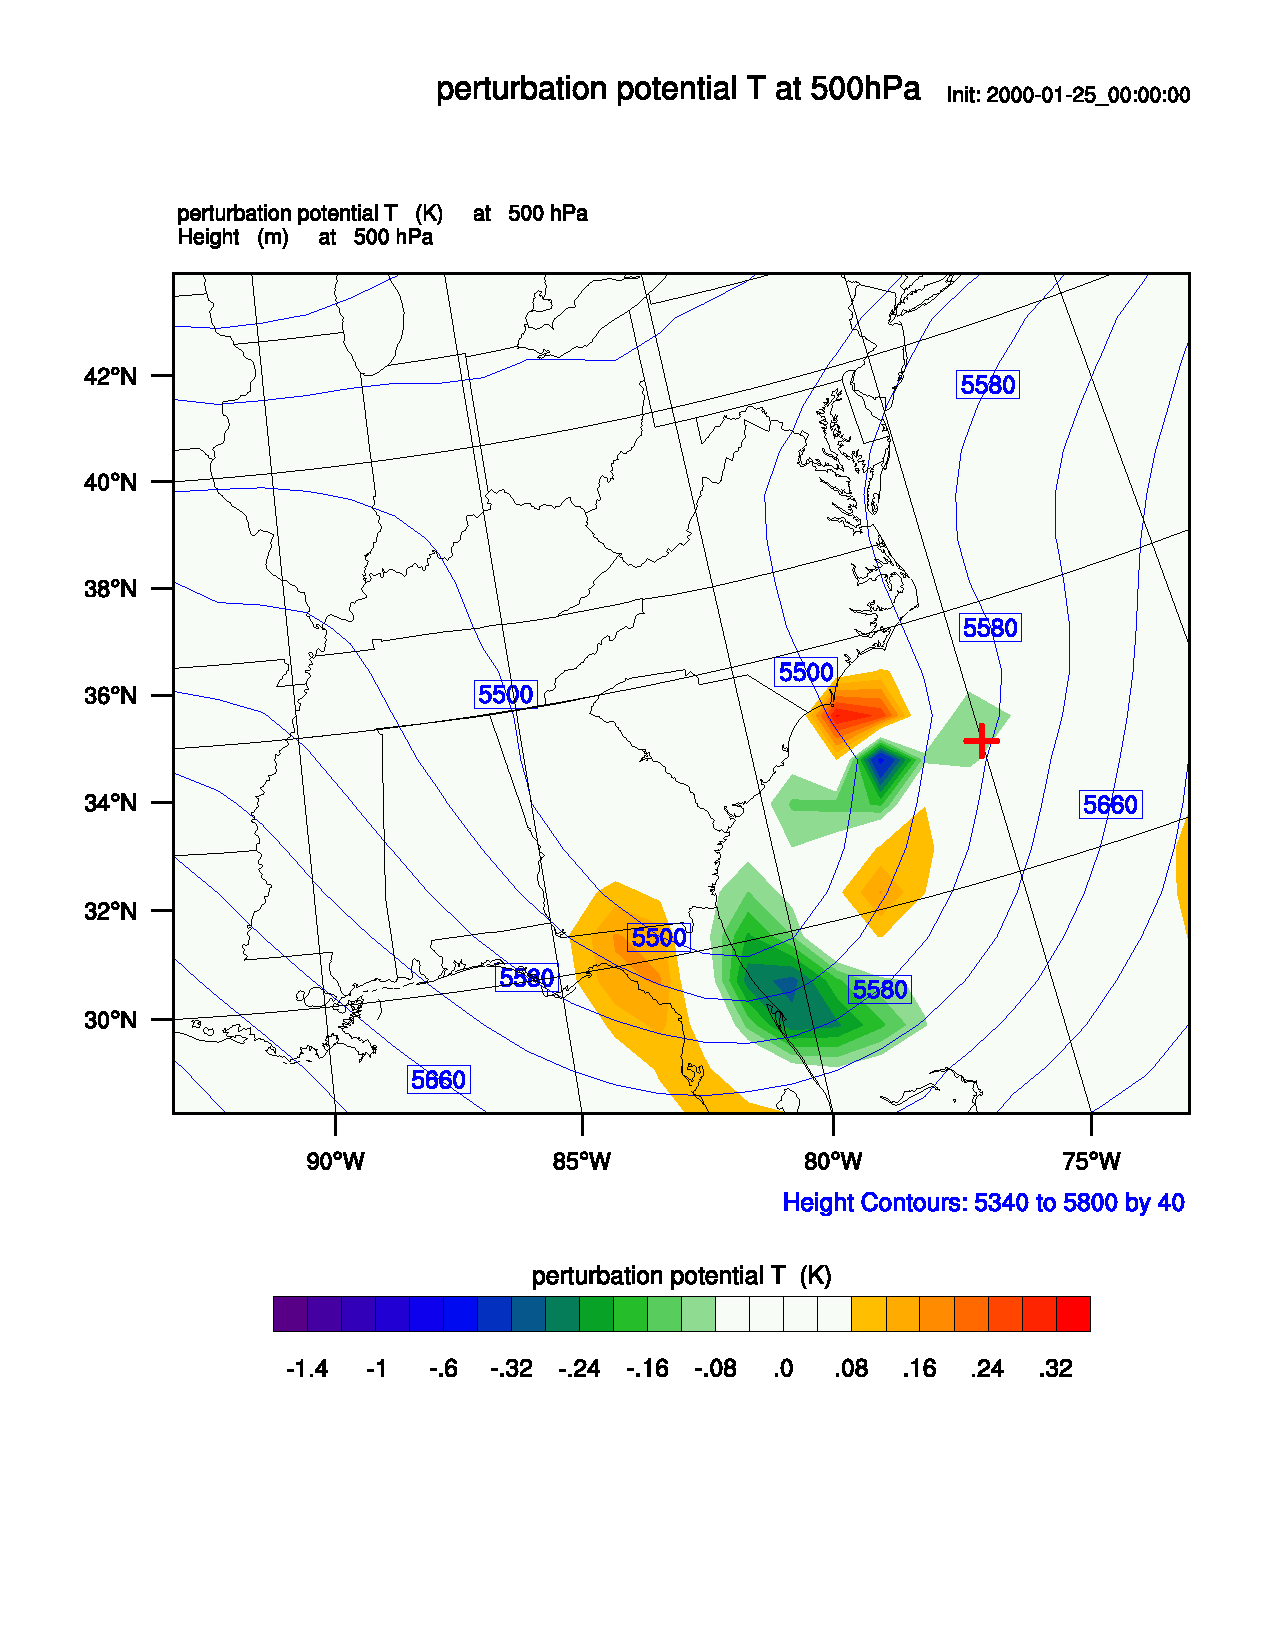
\includegraphics[trim=0 100 0 120, clip=true, width=0.90\textwidth]{figures/center}
			\caption {w/o LBC control}
		\end{figure}
	\end{column}
	\begin{column}{6cm}
		\begin{figure}
			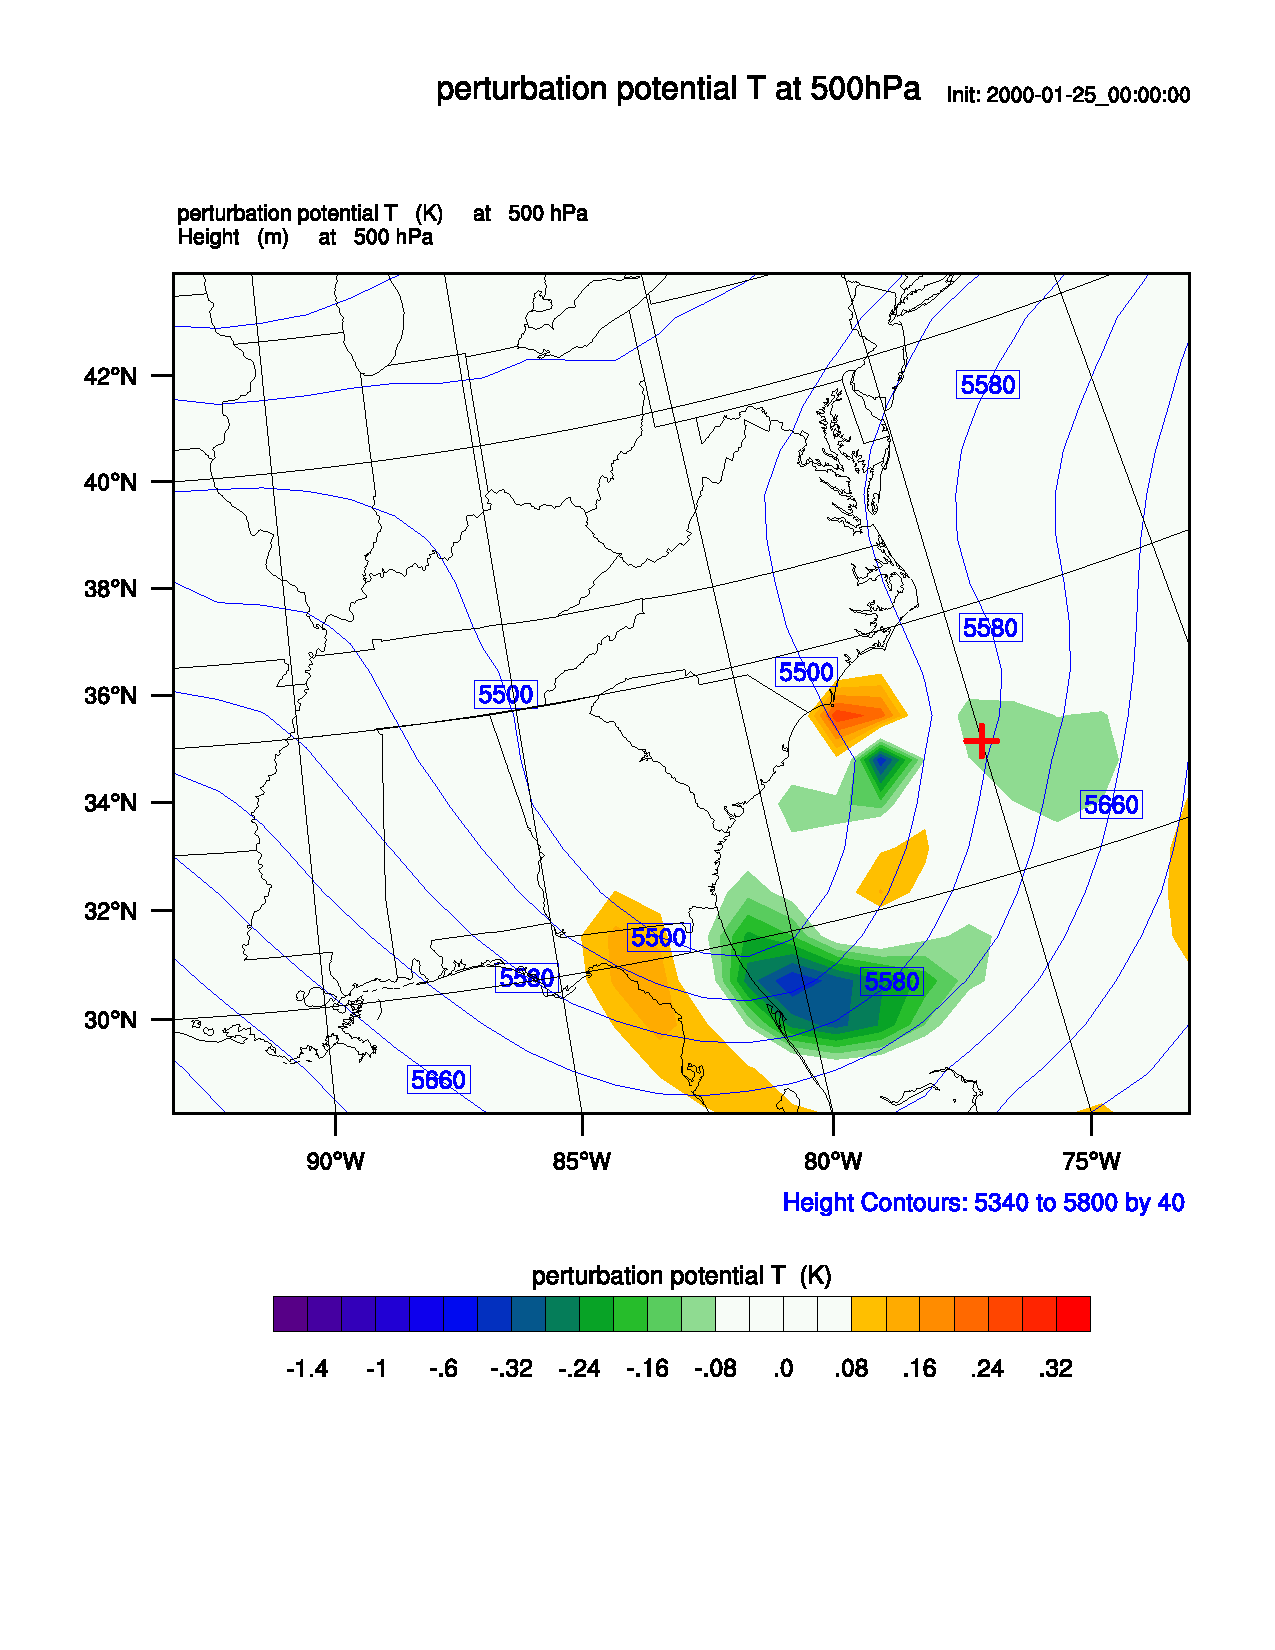
\includegraphics[trim=0 100 0 120, clip=true, width=0.90\textwidth]{figures/center_lbc}
			\caption {with LBC control}
		\end{figure}
	\end{column}
\end{columns}
\end{frame}

%\begin{frame}
%\frametitle{500hPa $\theta$ increments from 0--6 h w/o LBC control}
%\begin{figure} 
%\centering 
%\begin{minipage}[c]{0.3\linewidth} 
%\centering 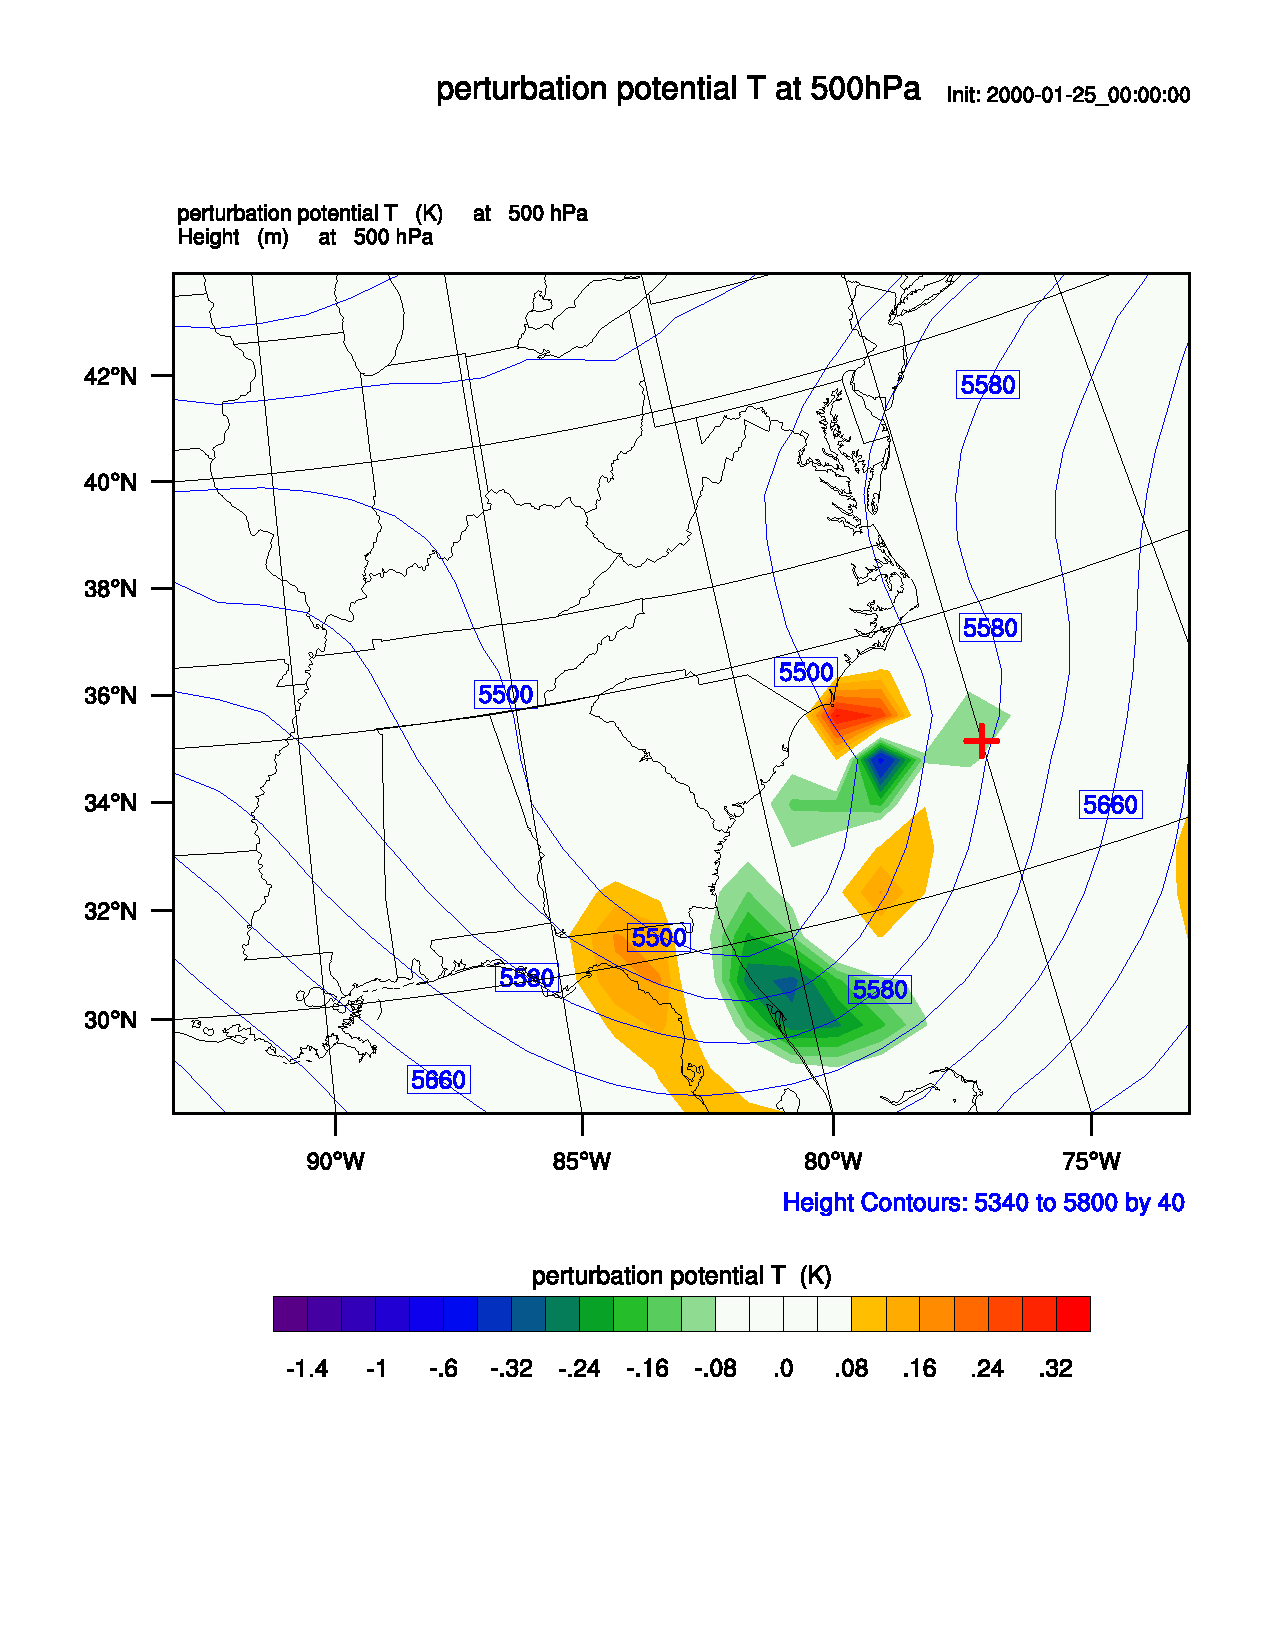
\includegraphics[trim=0 220 0 110, clip=true, width=1.0\textwidth]{figures/center} 
%\end{minipage}% 
%\begin{minipage}[c]{0.8\linewidth} 
%\centering 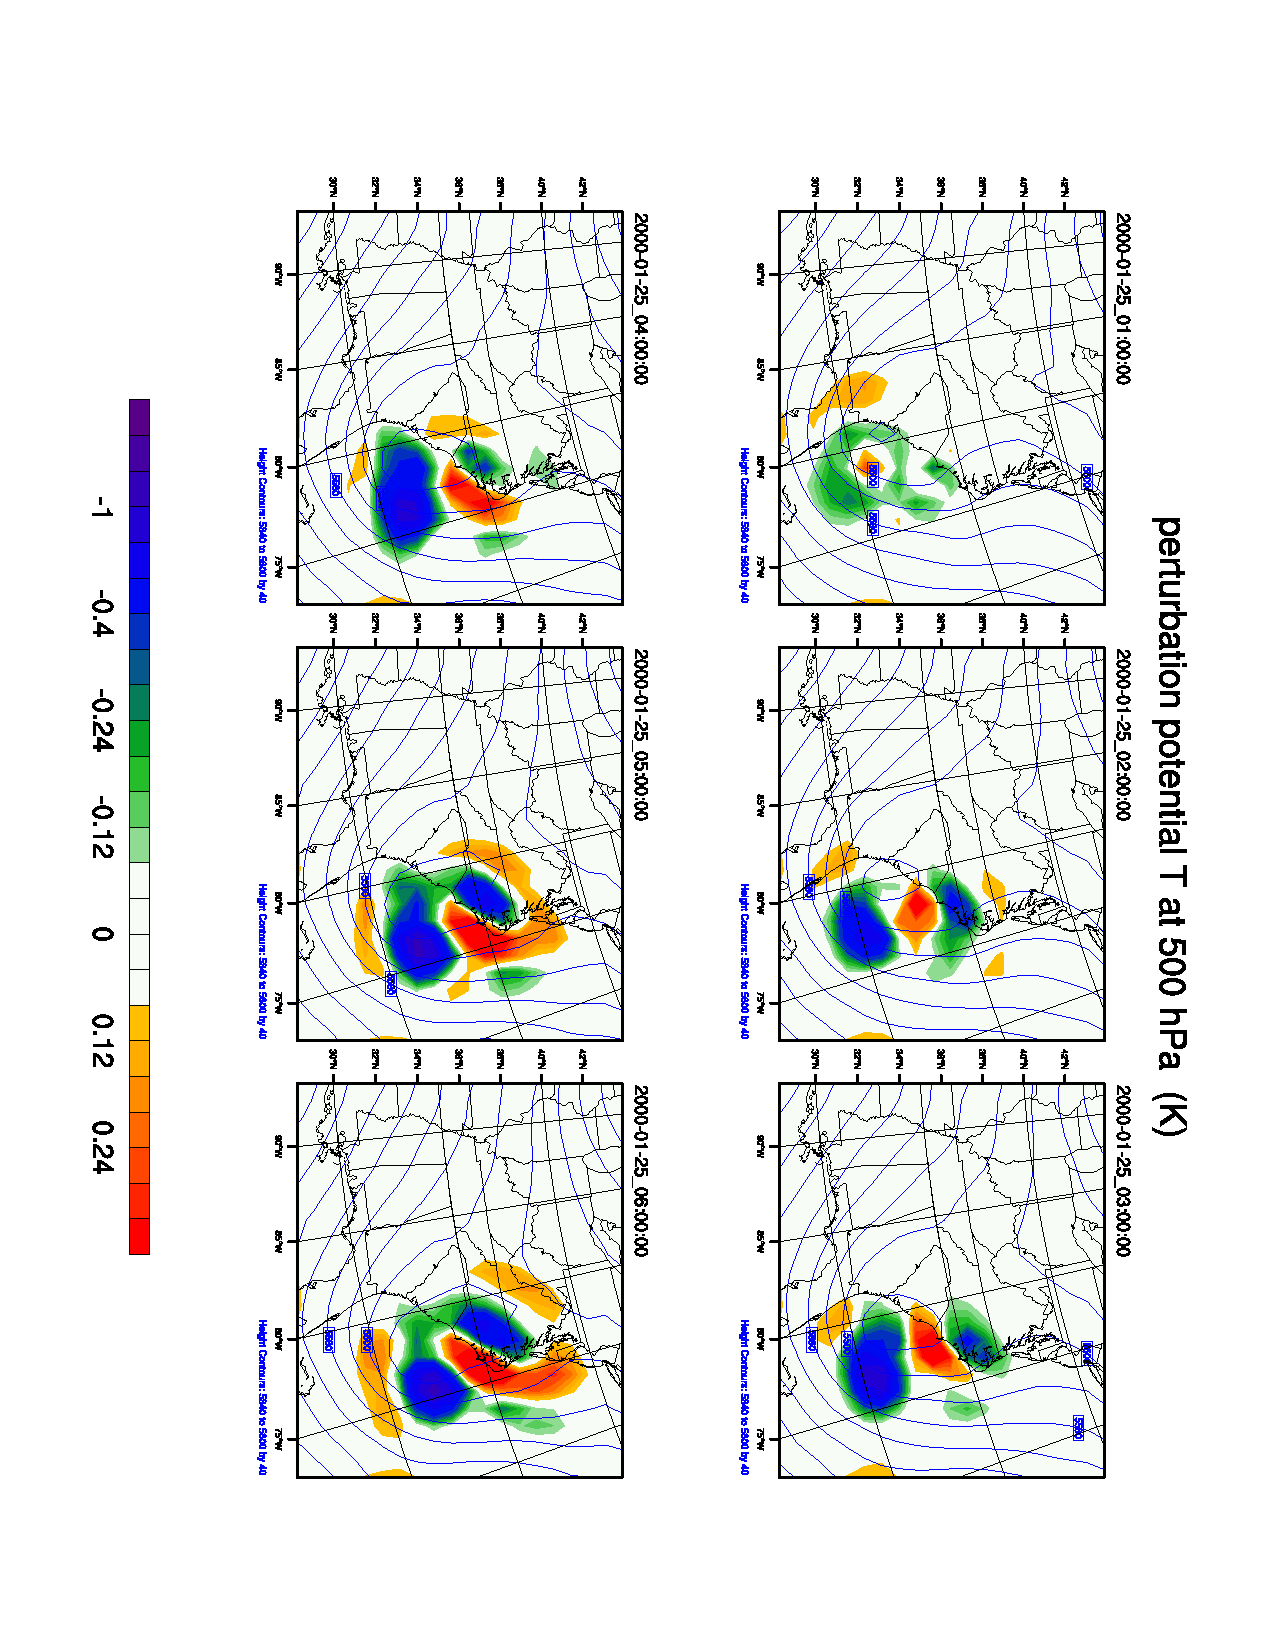
\includegraphics[trim=100 0 60 0, clip=true, angle=90, width=1.0\textwidth]{figures/center_6h} 
%\end{minipage} 
%\end{figure} 
%\end{frame}

\begin{frame}
\frametitle{500hPa $\theta$ increments from 0--6 h w/o LBC control}
\begin{figure} 
\centering 
\centering 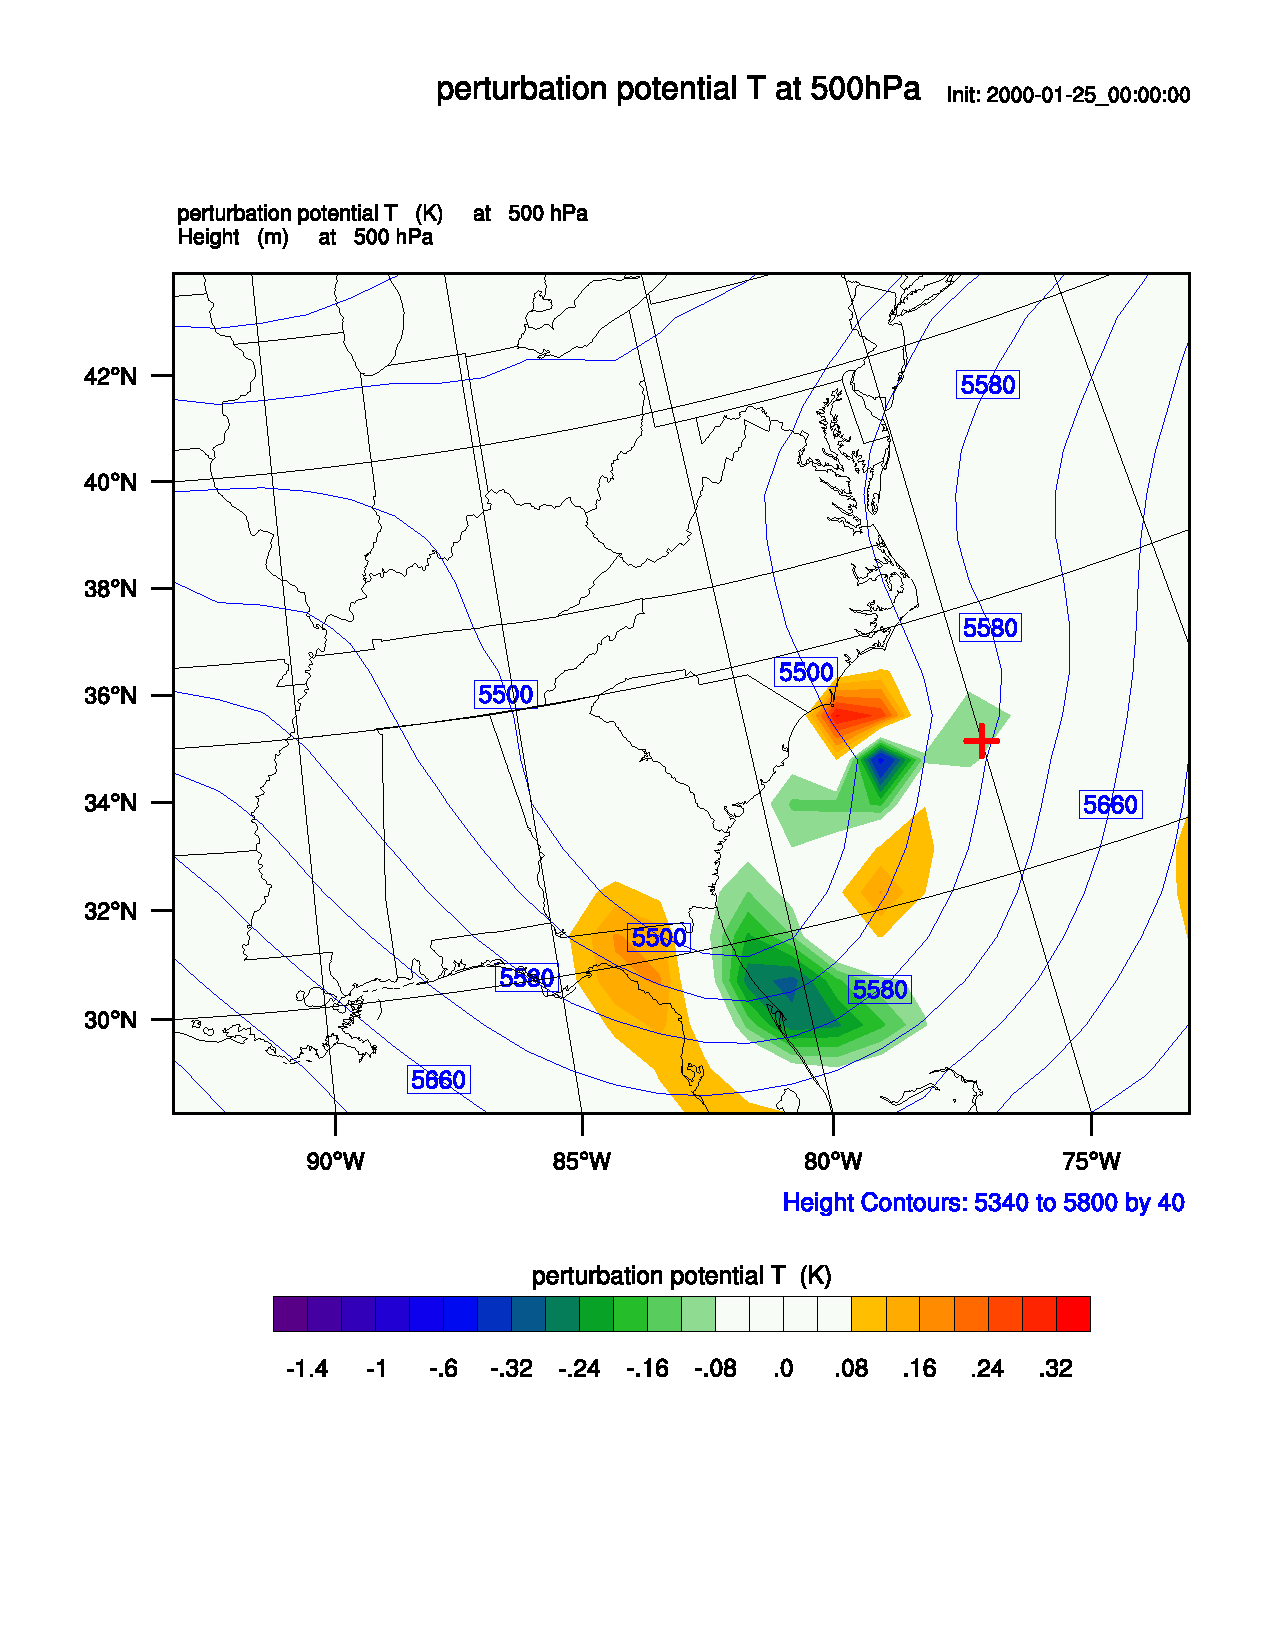
\includegraphics[trim=40 230 40 110, clip=true, width=0.7\textwidth]{figures/center} 
\end{figure} 
\end{frame}

\begin{frame}
\frametitle{500hPa $\theta$ increments from 0--6 h w/o LBC control}
\begin{figure} 
\centering 
\centering 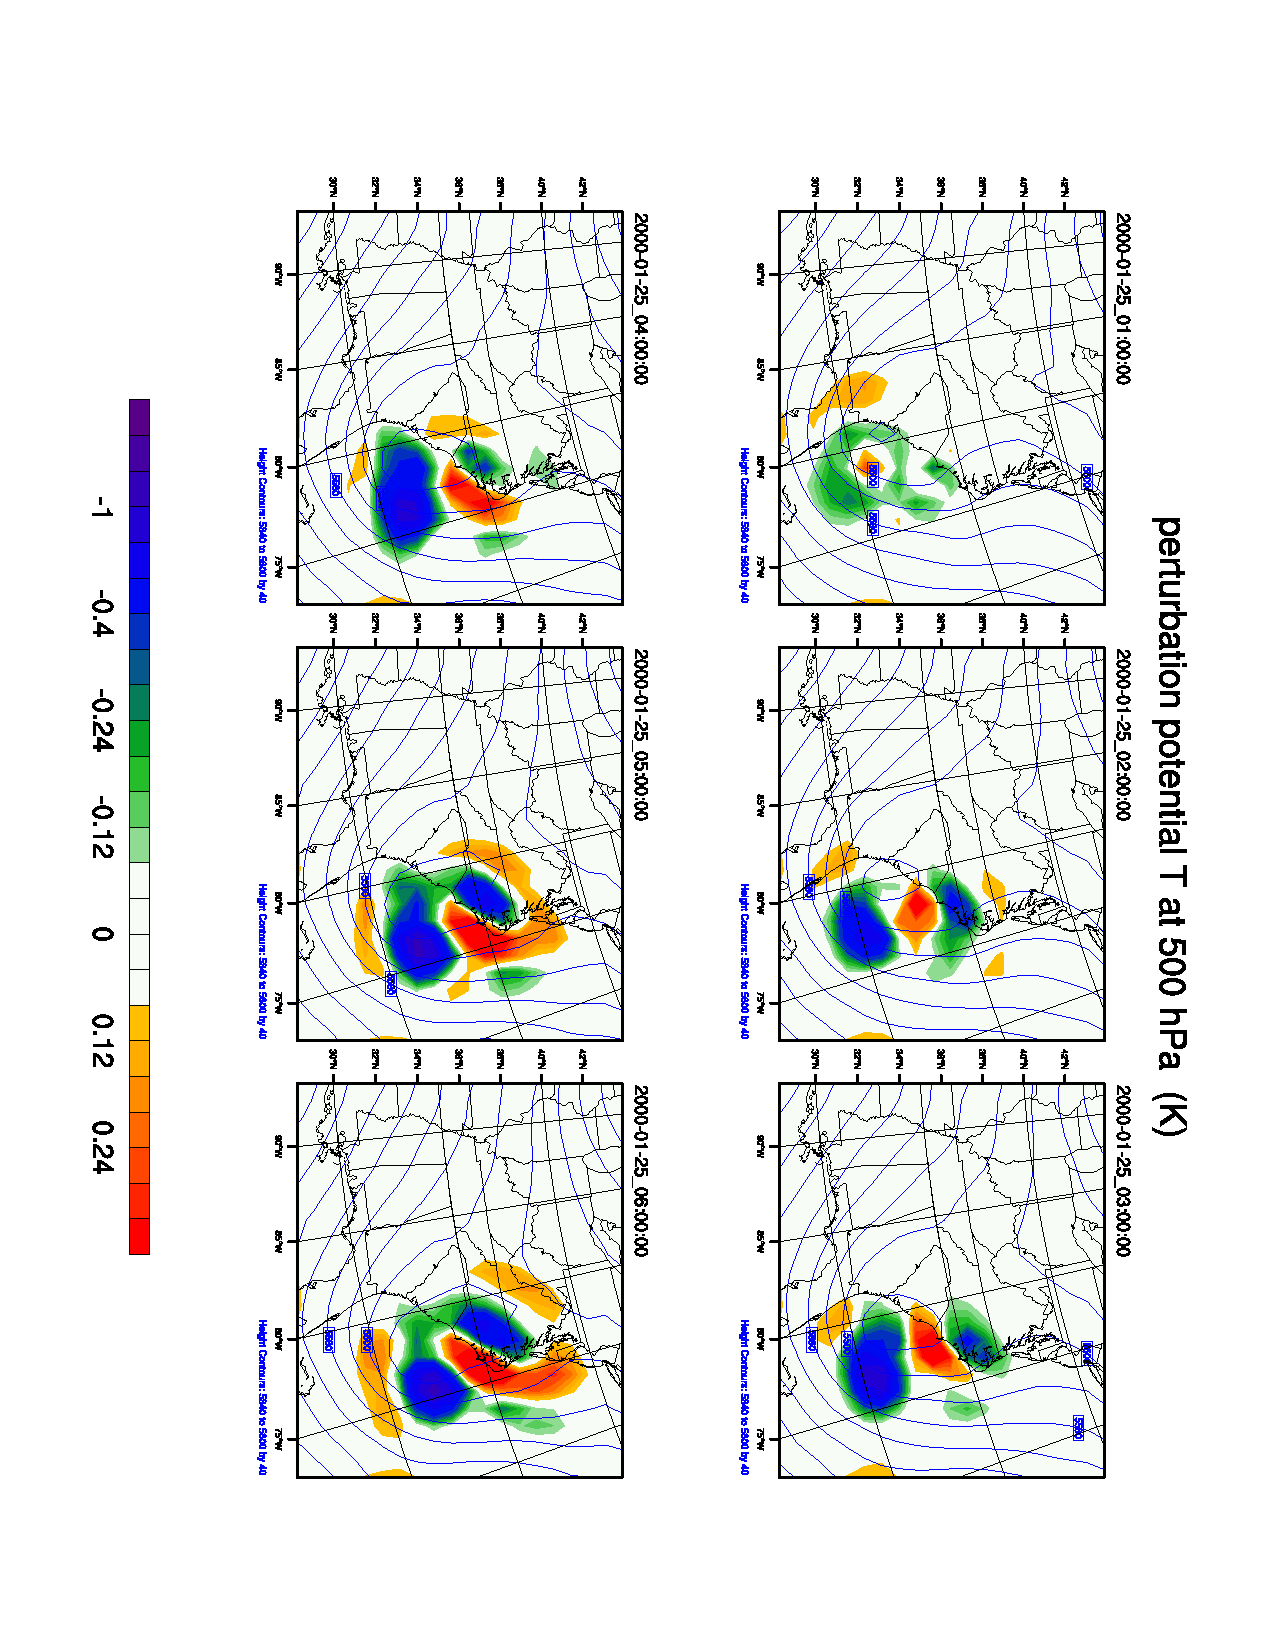
\includegraphics[trim=363 500 66 85, clip=true, angle=90, width=0.7\textwidth]{figures/center_6h} 
\end{figure} 
\end{frame}

\begin{frame}
\frametitle{500hPa $\theta$ increments from 0--6 h w/o LBC control}
\begin{figure} 
\centering 
\centering 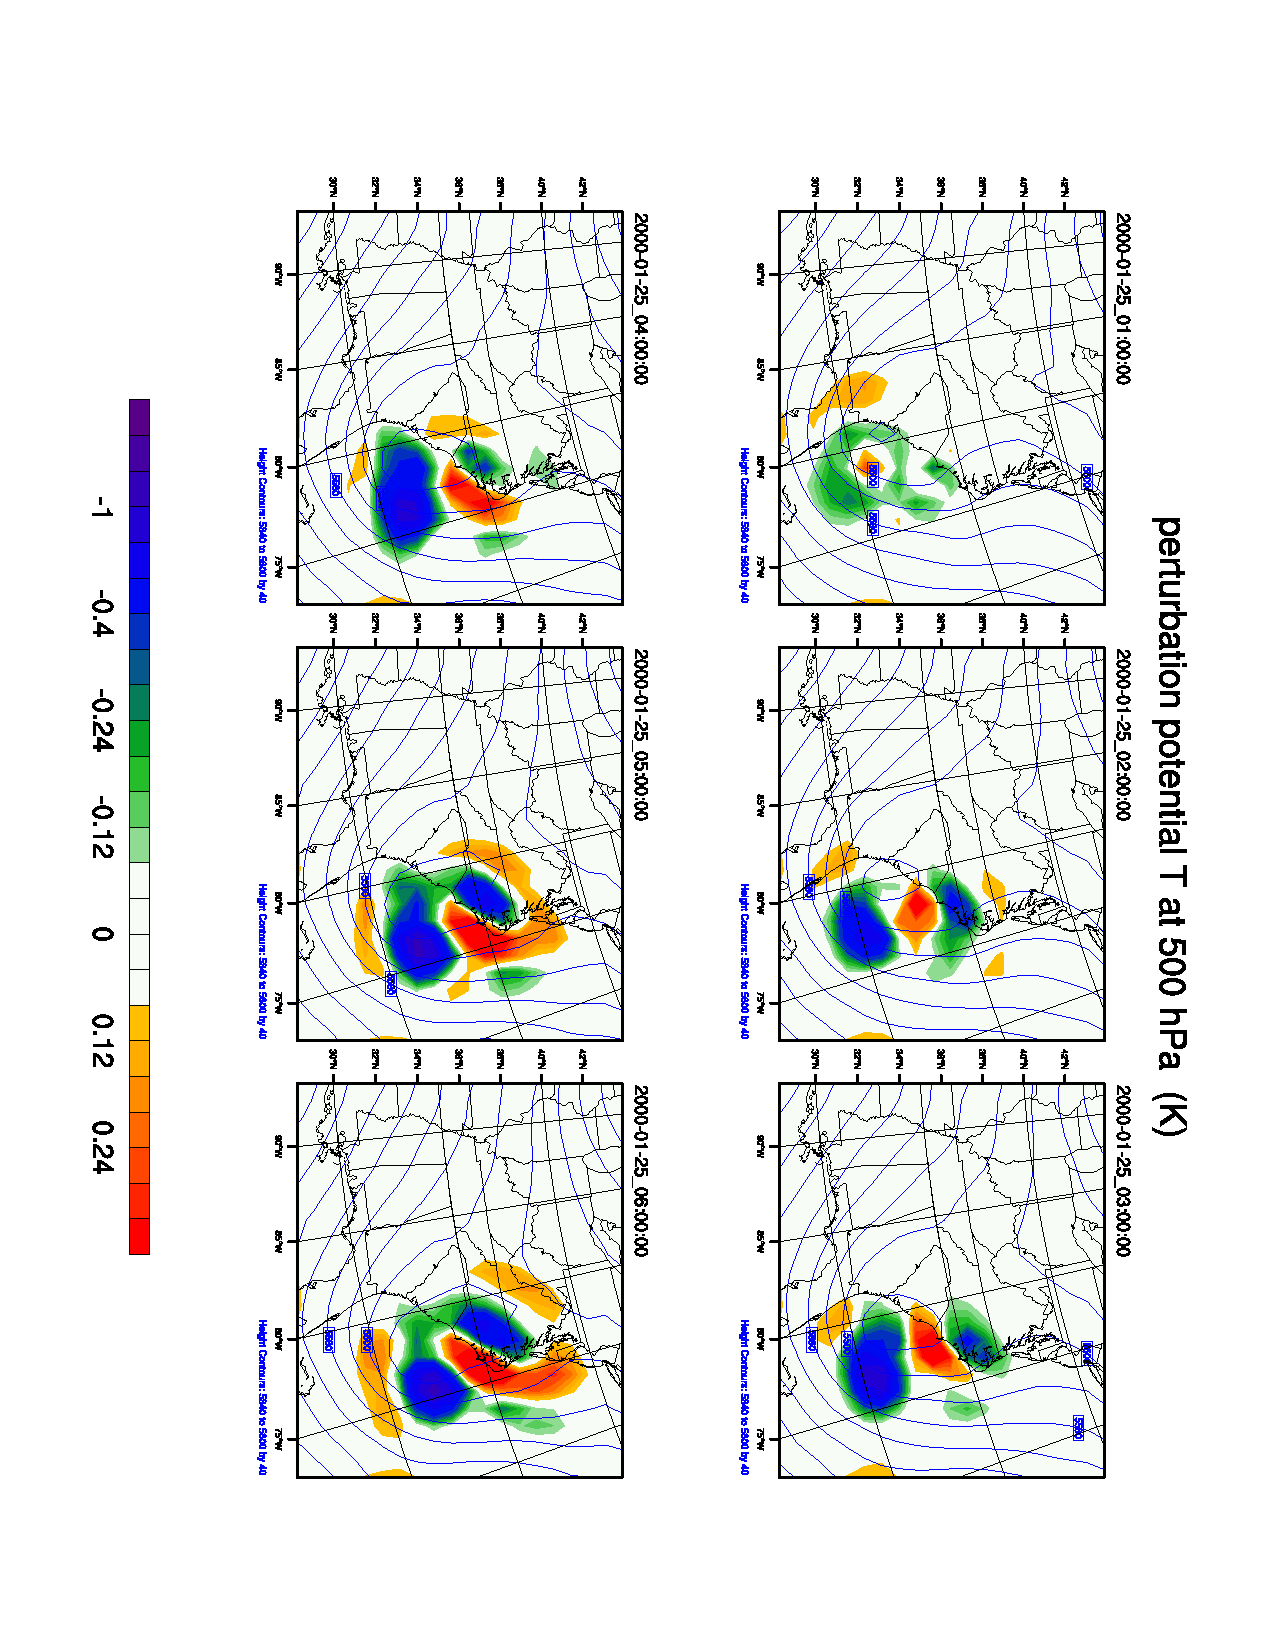
\includegraphics[trim=363 291 66 295, clip=true, angle=90, width=0.7\textwidth]{figures/center_6h} 
\end{figure} 
\end{frame}

\begin{frame}
\frametitle{500hPa $\theta$ increments from 0--6 h w/o LBC control}
\begin{figure} 
\centering 
\centering 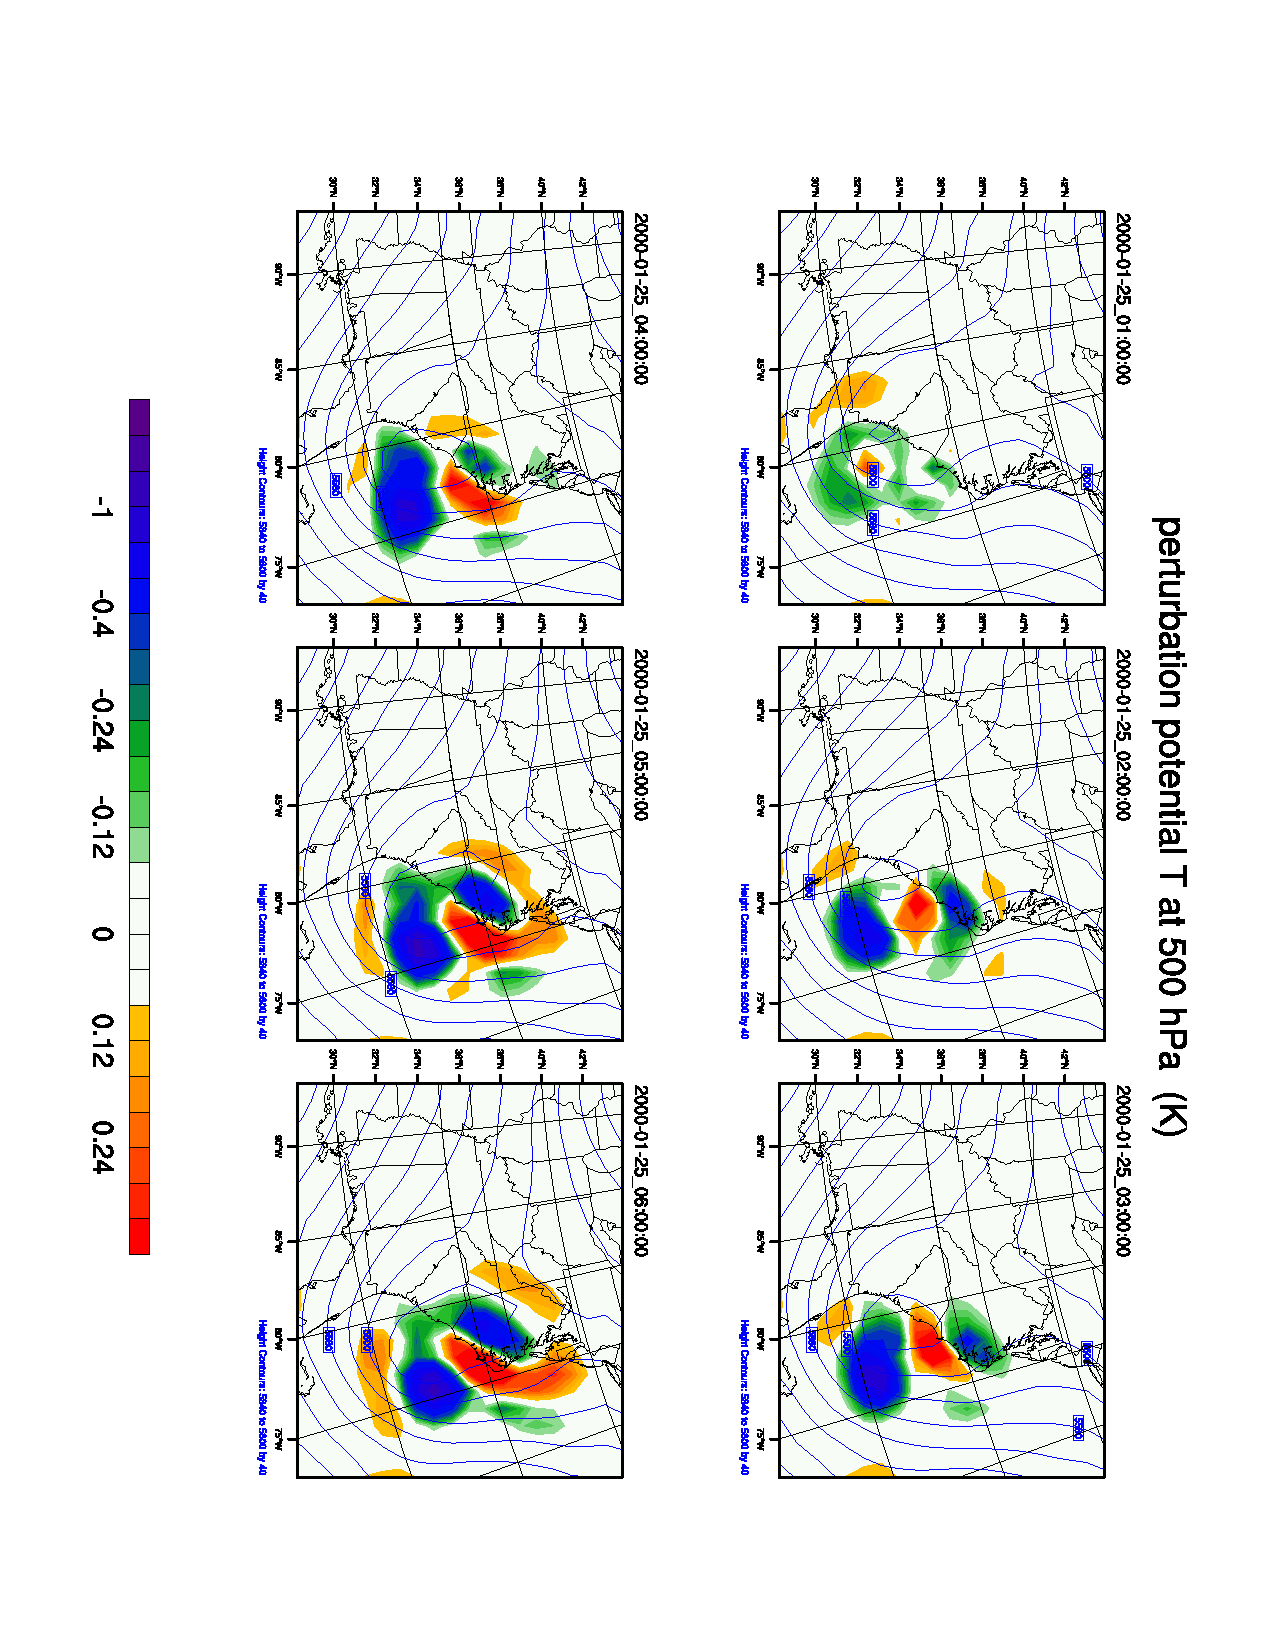
\includegraphics[trim=363 82 66 502, clip=true, angle=90, width=0.7\textwidth]{figures/center_6h} 
\end{figure} 
\end{frame}

\begin{frame}
\frametitle{500hPa $\theta$ increments from 0--6 h w/o LBC control}
\begin{figure} 
\centering 
\centering 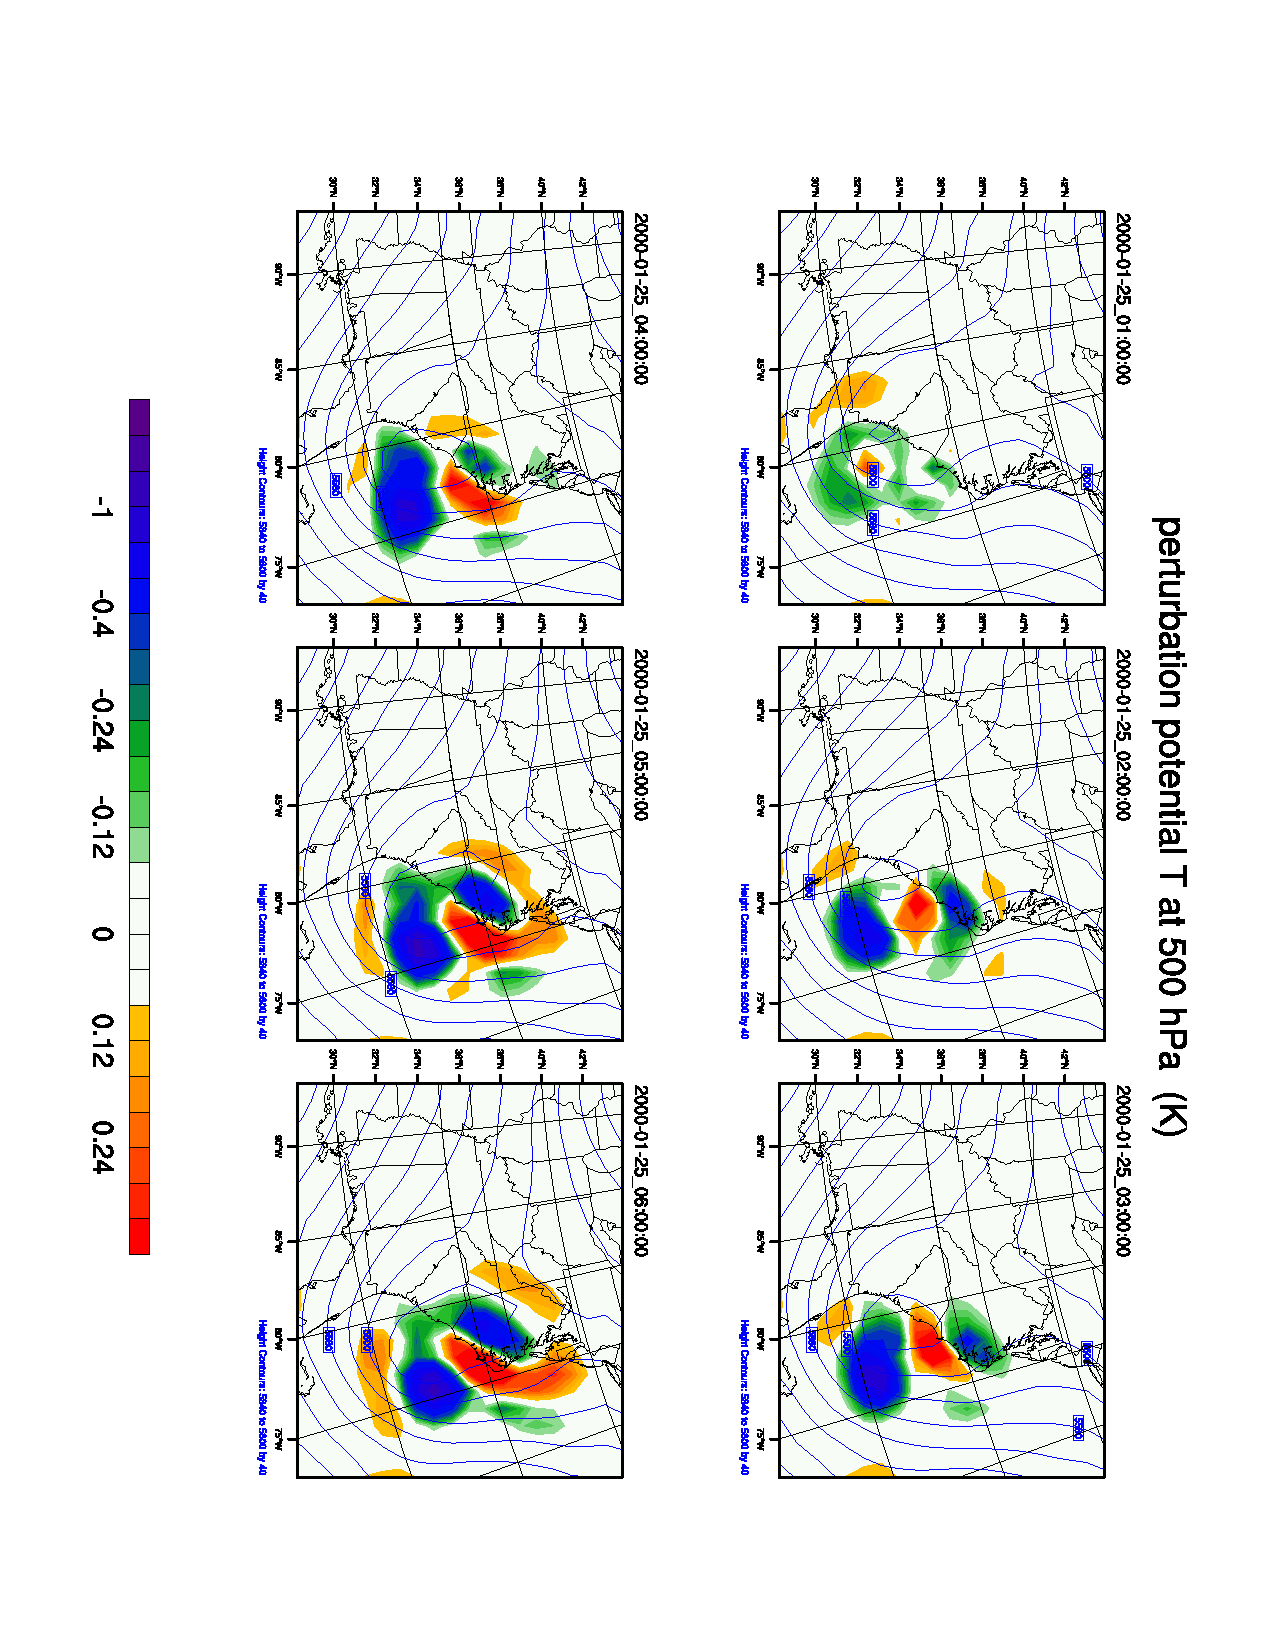
\includegraphics[trim=132 500 300 85, clip=true, angle=90, width=0.7\textwidth]{figures/center_6h} 
\end{figure} 
\end{frame}

\begin{frame}
\frametitle{500hPa $\theta$ increments from 0--6 h w/o LBC control}
\begin{figure} 
\centering 
\centering 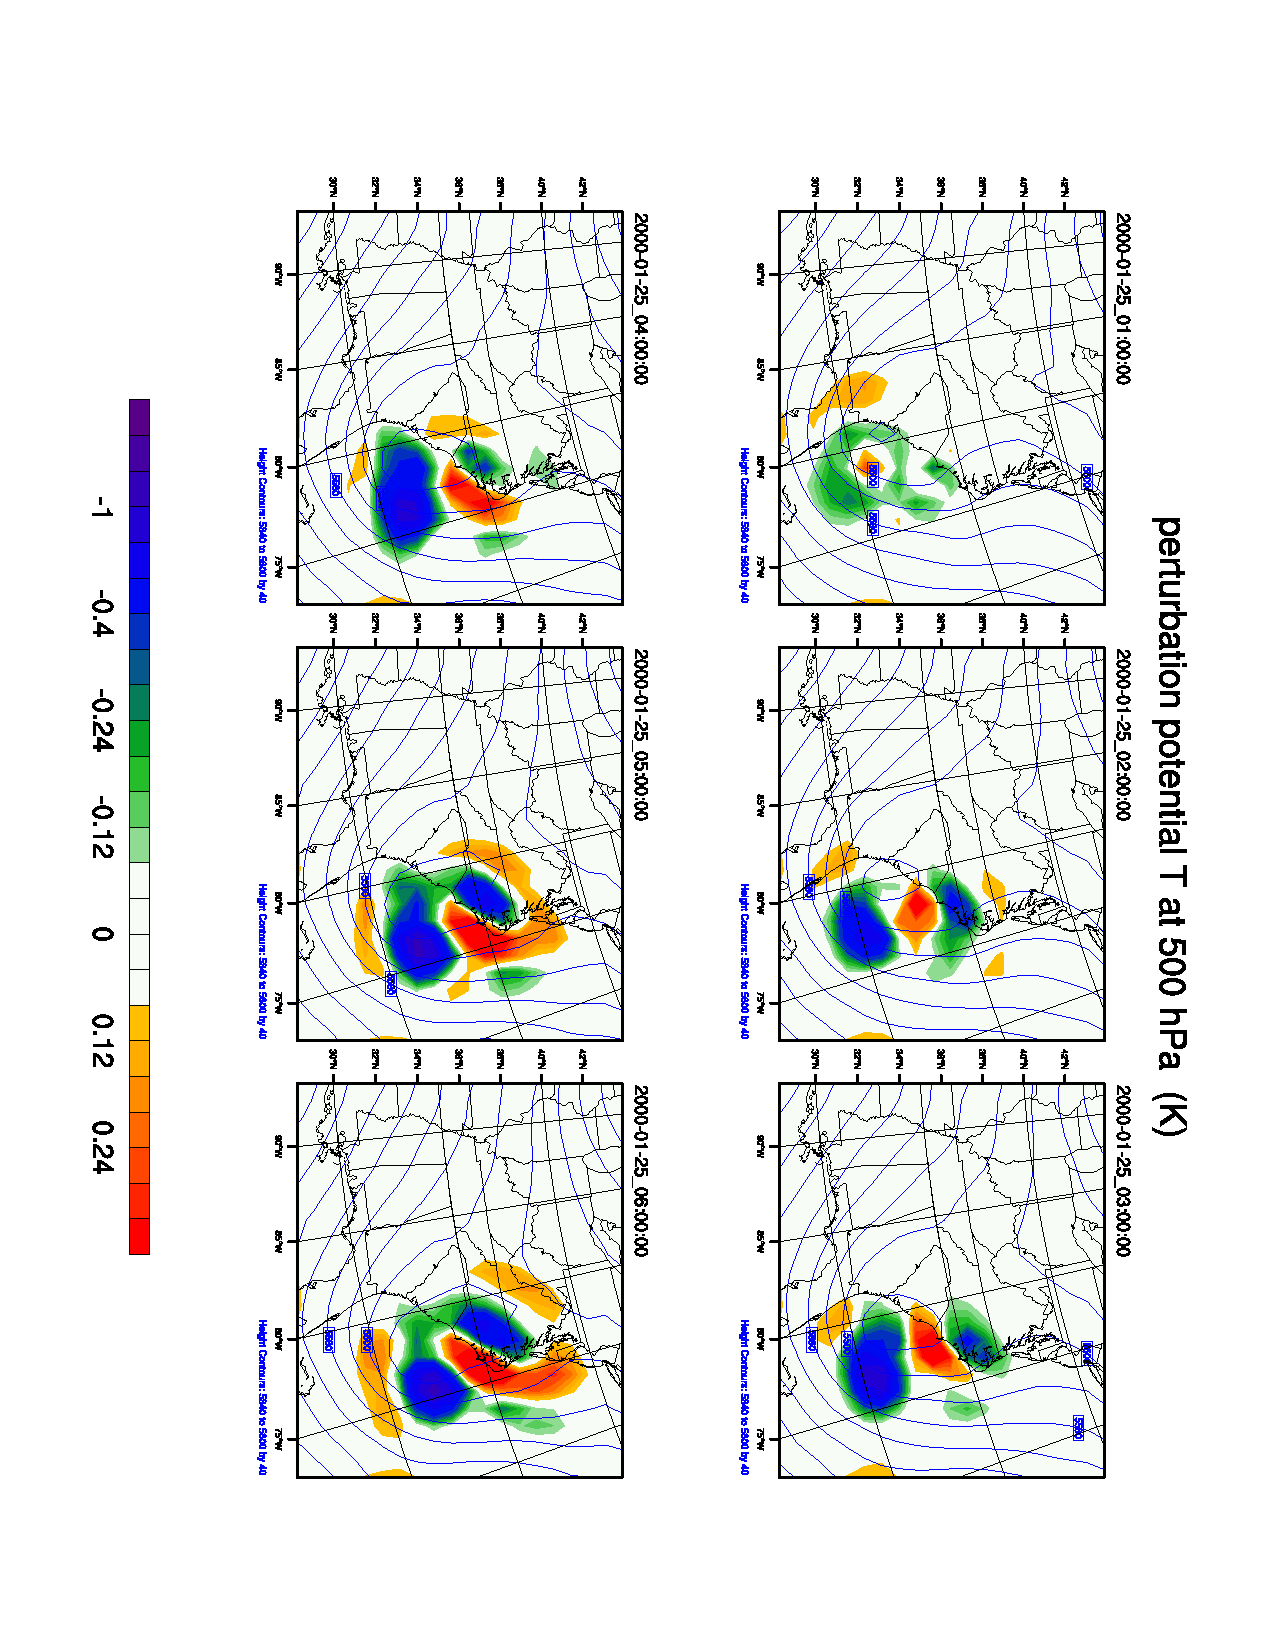
\includegraphics[trim=132 291 300 293, clip=true, angle=90, width=0.7\textwidth]{figures/center_6h} 
\end{figure} 
\end{frame}

\begin{frame}
\frametitle{500hPa $\theta$ increments from 0--6 h w/o LBC control}
\begin{figure} 
\centering 
\centering 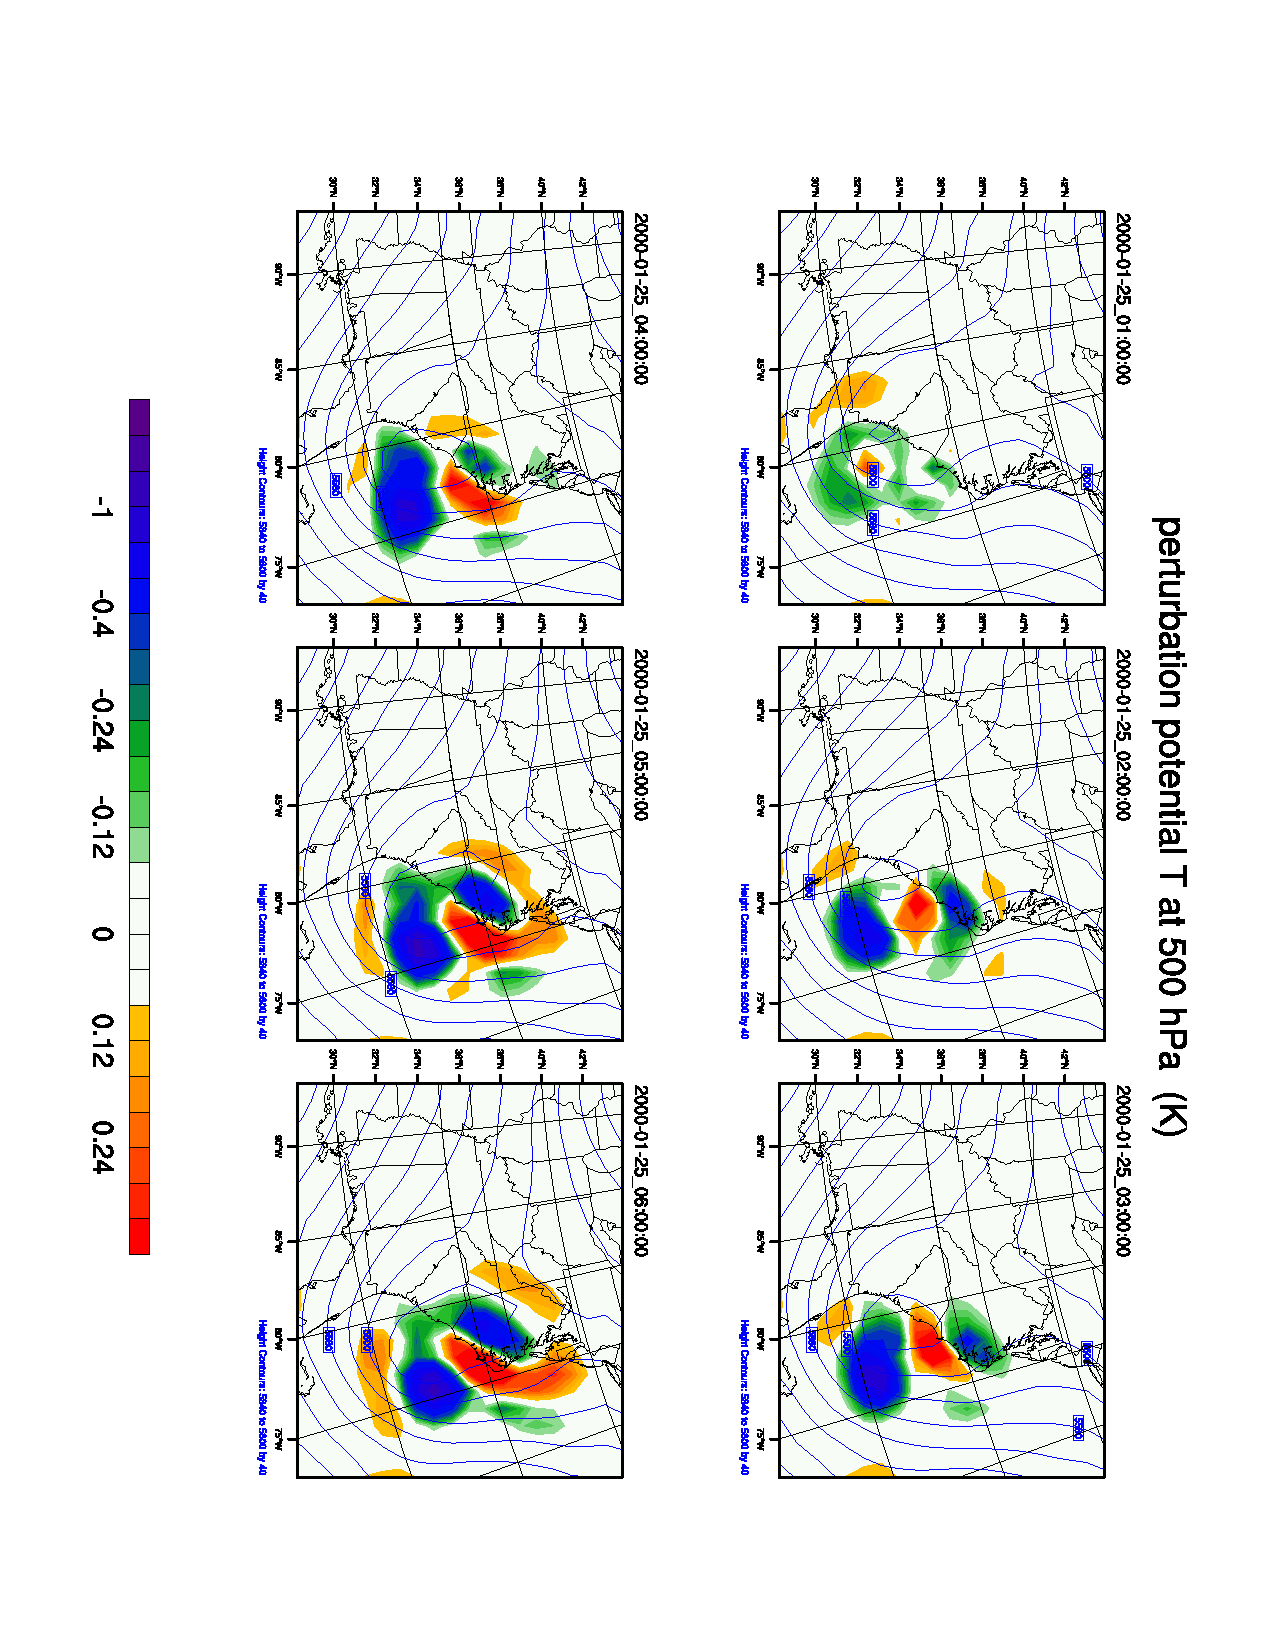
\includegraphics[trim=132 82 300 502, clip=true, angle=90, width=0.7\textwidth]{figures/center_6h} 
\end{figure} 
\end{frame}

%\begin{frame}
%\frametitle{500hPa $\theta$ increments from 0--6 h with LBC control}
%\animate<2-4>
%\begin{figure} 
%\centering 
%\begin{minipage}[c]{0.3\linewidth} 
%\centering 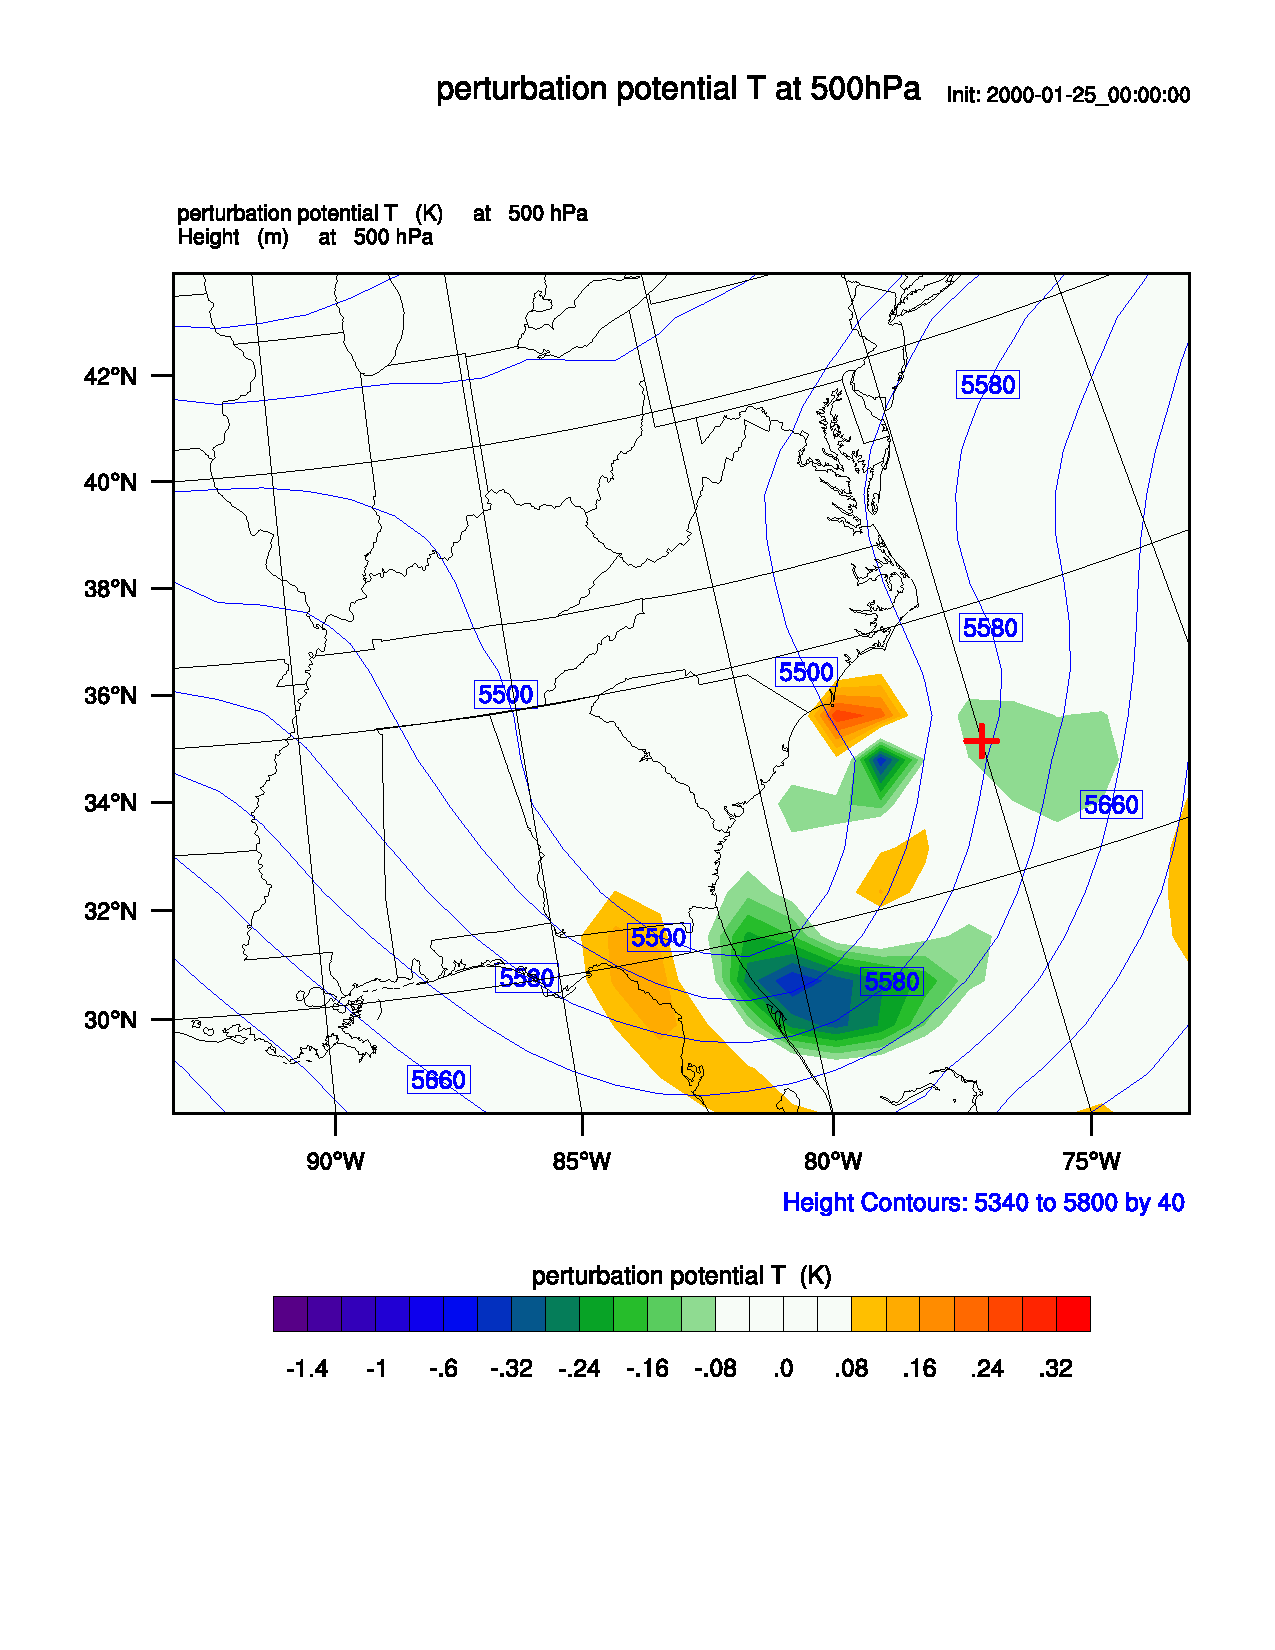
\includegraphics[trim=0 220 0 110, clip=true, width=1.0\textwidth]{figures/center_lbc} 
%\end{minipage}% 
%\begin{minipage}[c]{0.8\linewidth} 
%\centering 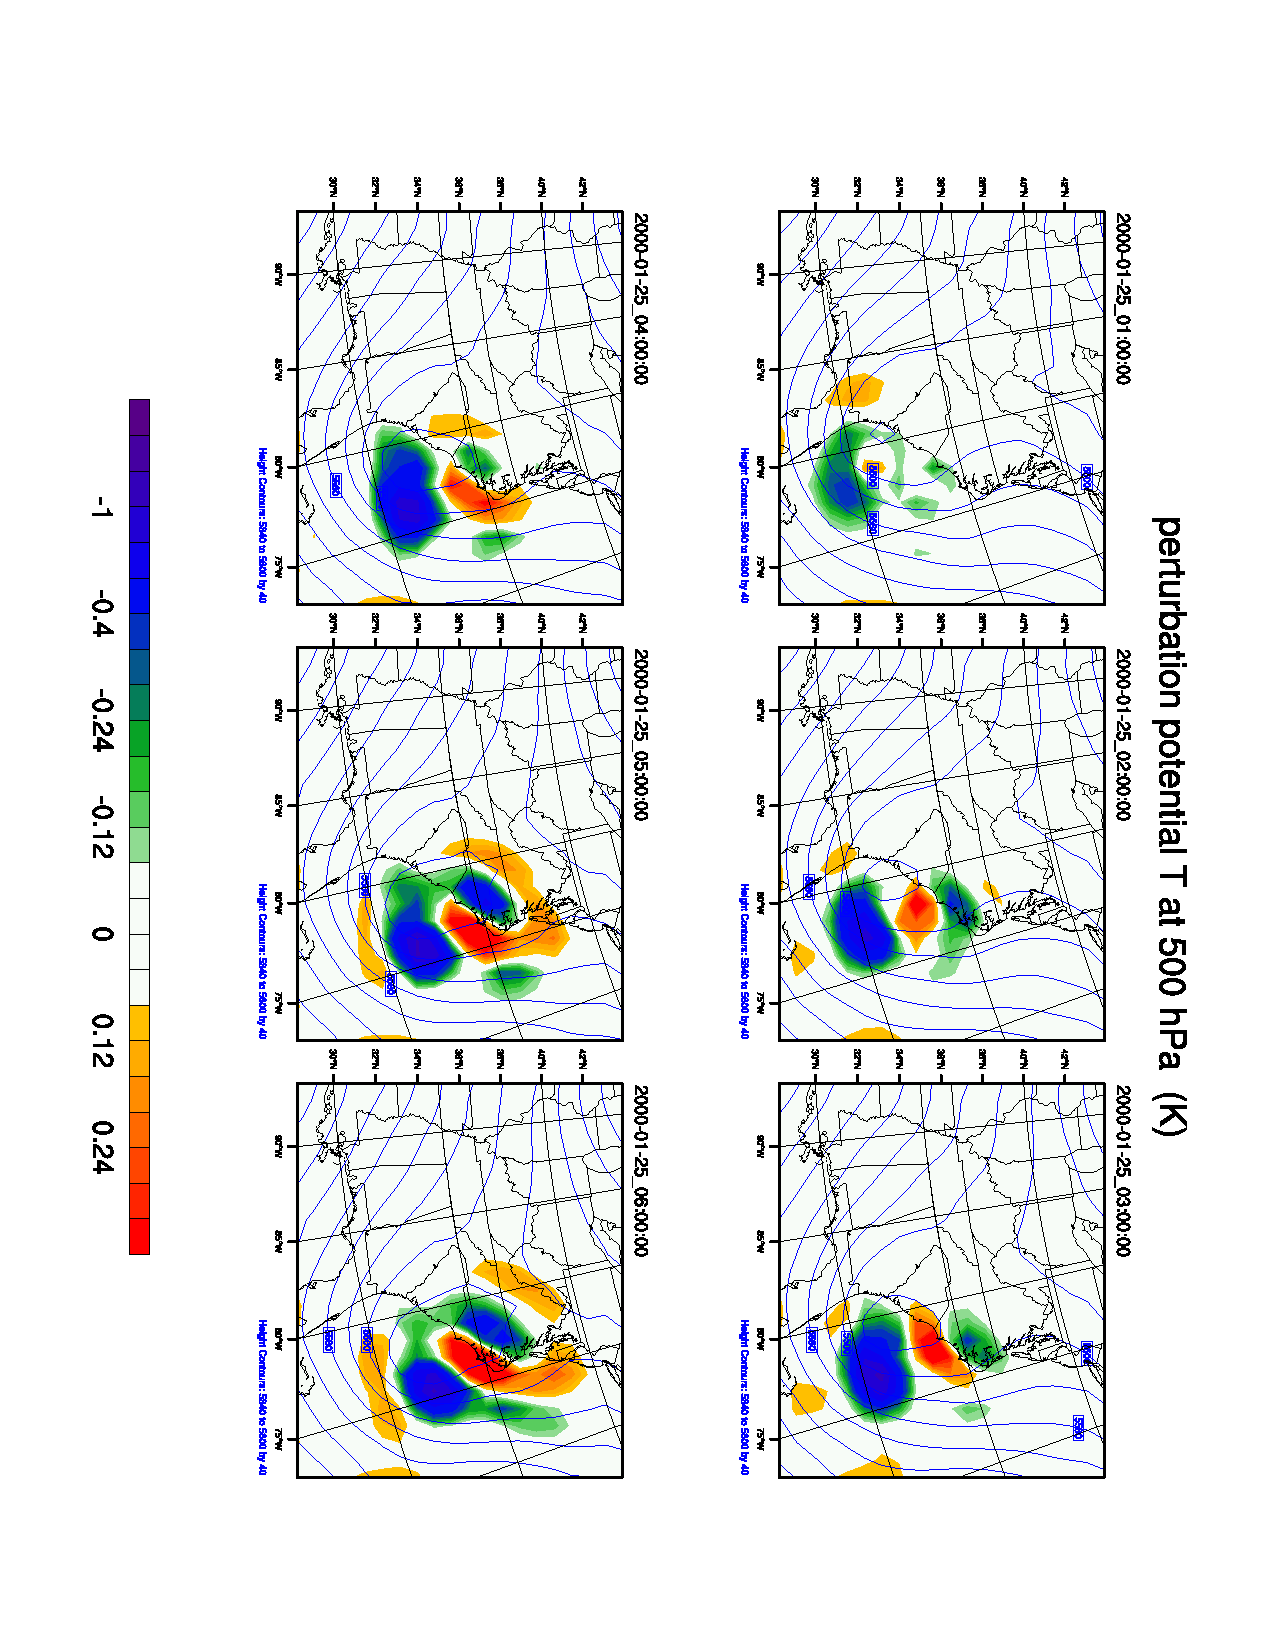
\includegraphics[trim=100 0 60 0, clip=true, angle=90, width=1.0\textwidth]{figures/center_lbc_6h} 
%\end{minipage} 
%\end{figure} 
%\end{frame}

\begin{frame}
\frametitle{500hPa $\theta$ increments from 0--6 h with LBC control}
\begin{figure} 
\centering 
\centering 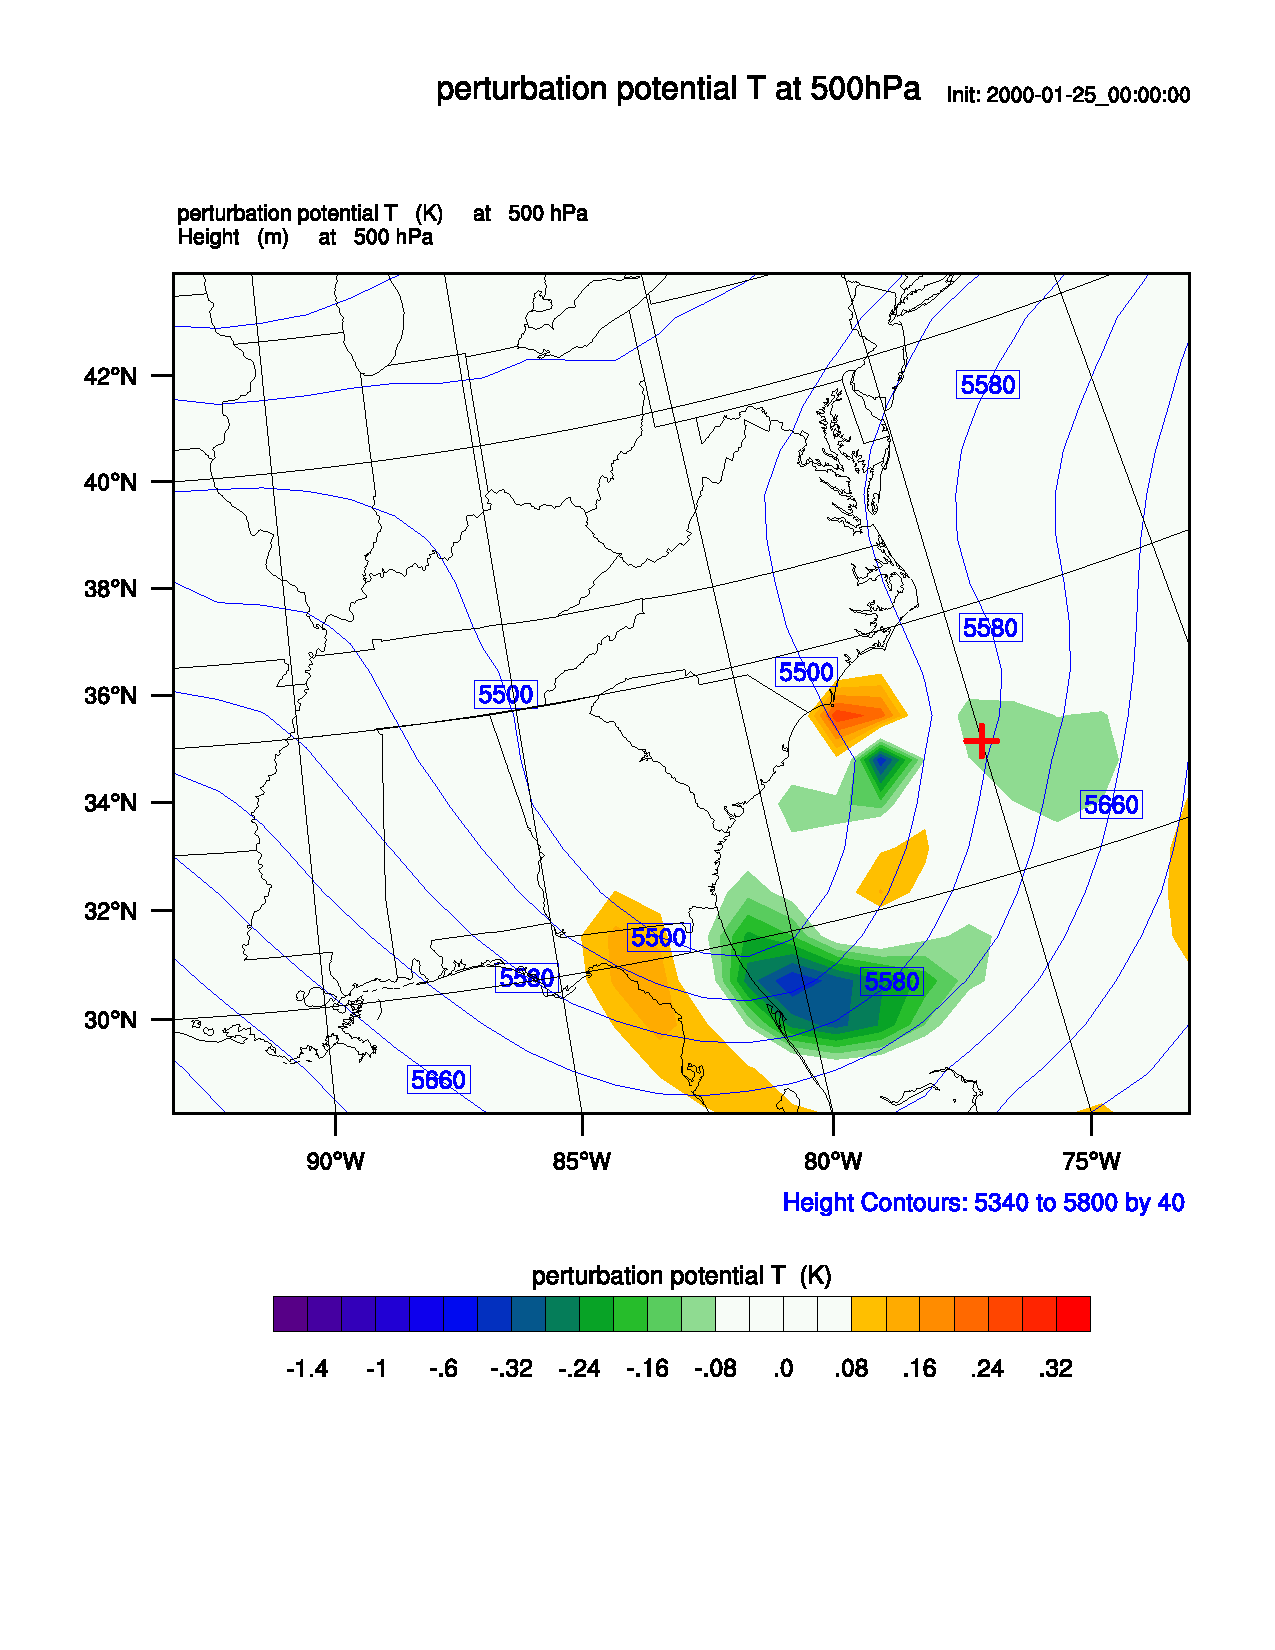
\includegraphics[trim=40 230 40 110, clip=true, width=0.7\textwidth]{figures/center_lbc} 
\end{figure} 
\end{frame}

\begin{frame}
\frametitle{500hPa $\theta$ increments from 0--6 h with LBC control}
\begin{figure} 
\centering 
\centering 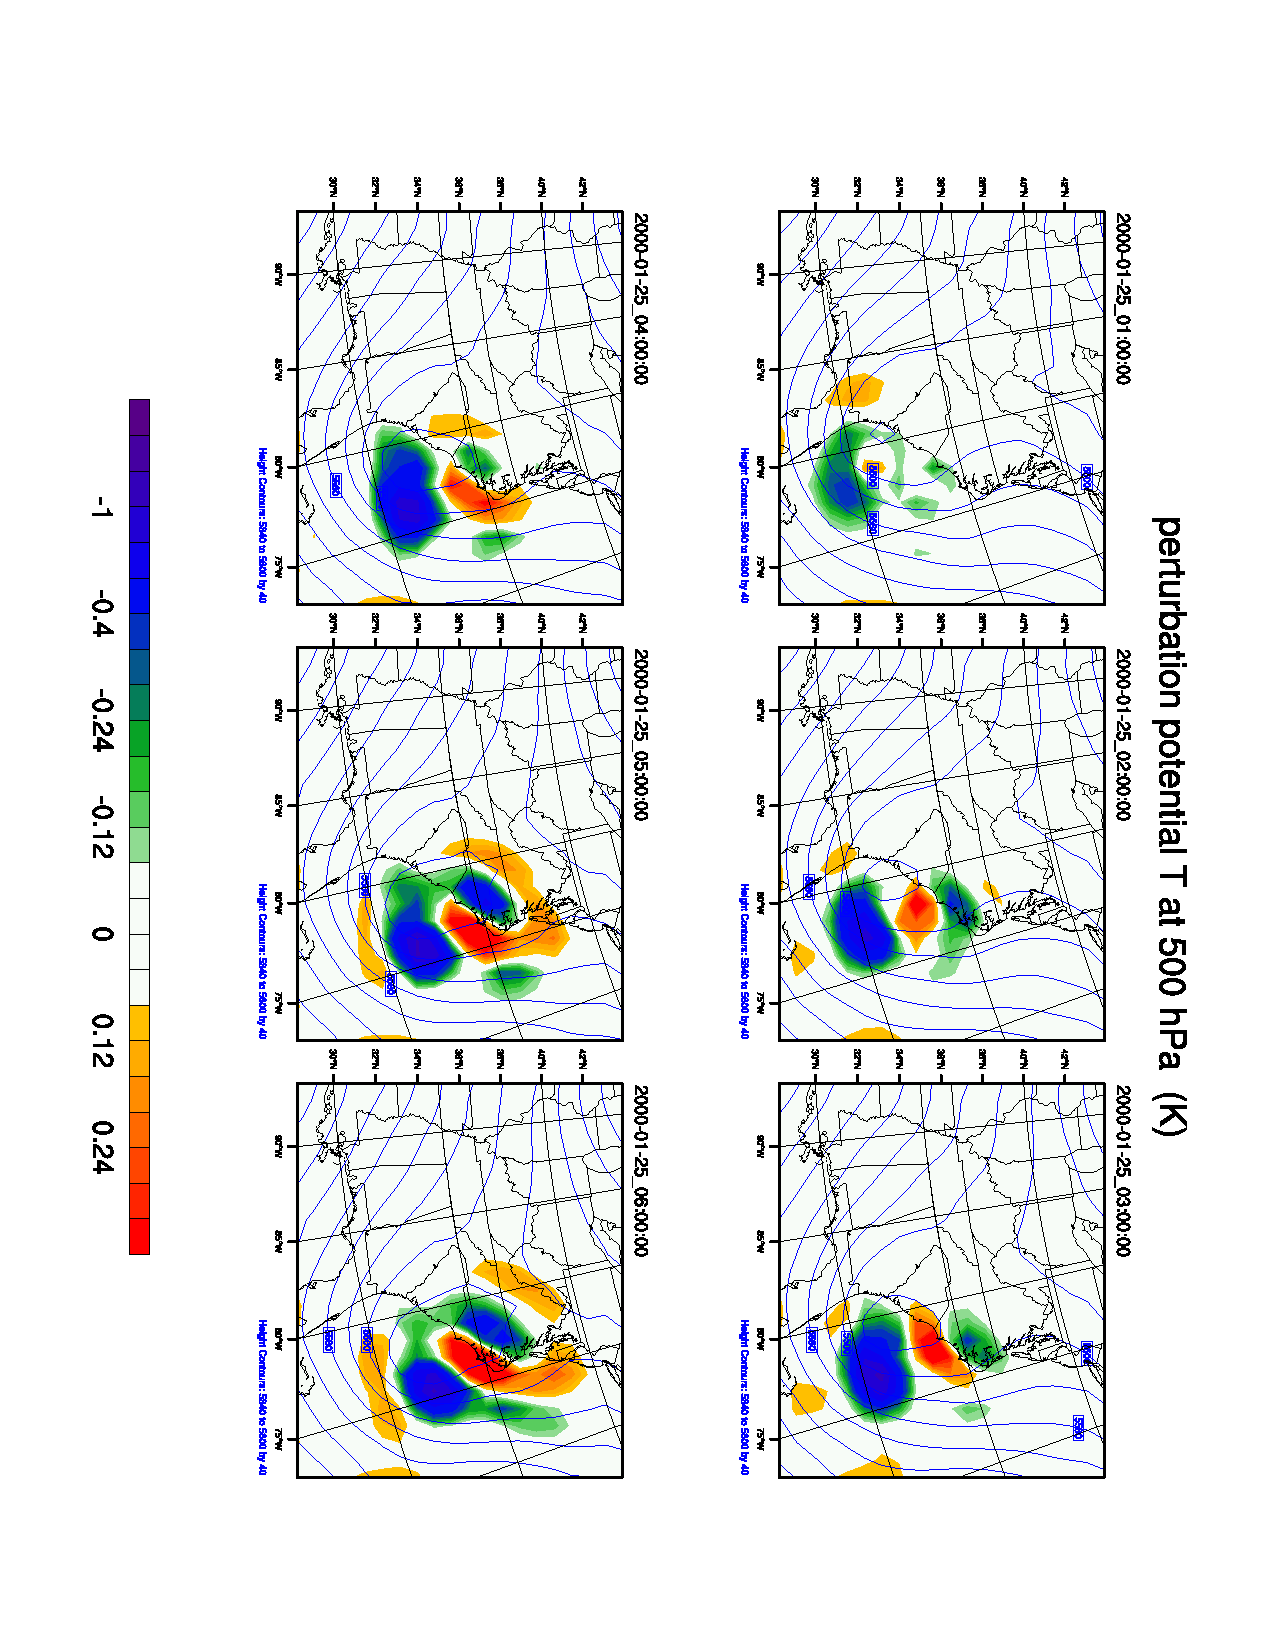
\includegraphics[trim=363 500 66 85, clip=true, angle=90, width=0.7\textwidth]{figures/center_lbc_6h} 
\end{figure} 
\end{frame}

\begin{frame}
\frametitle{500hPa $\theta$ increments from 0--6 h with LBC control}
\begin{figure} 
\centering 
\centering 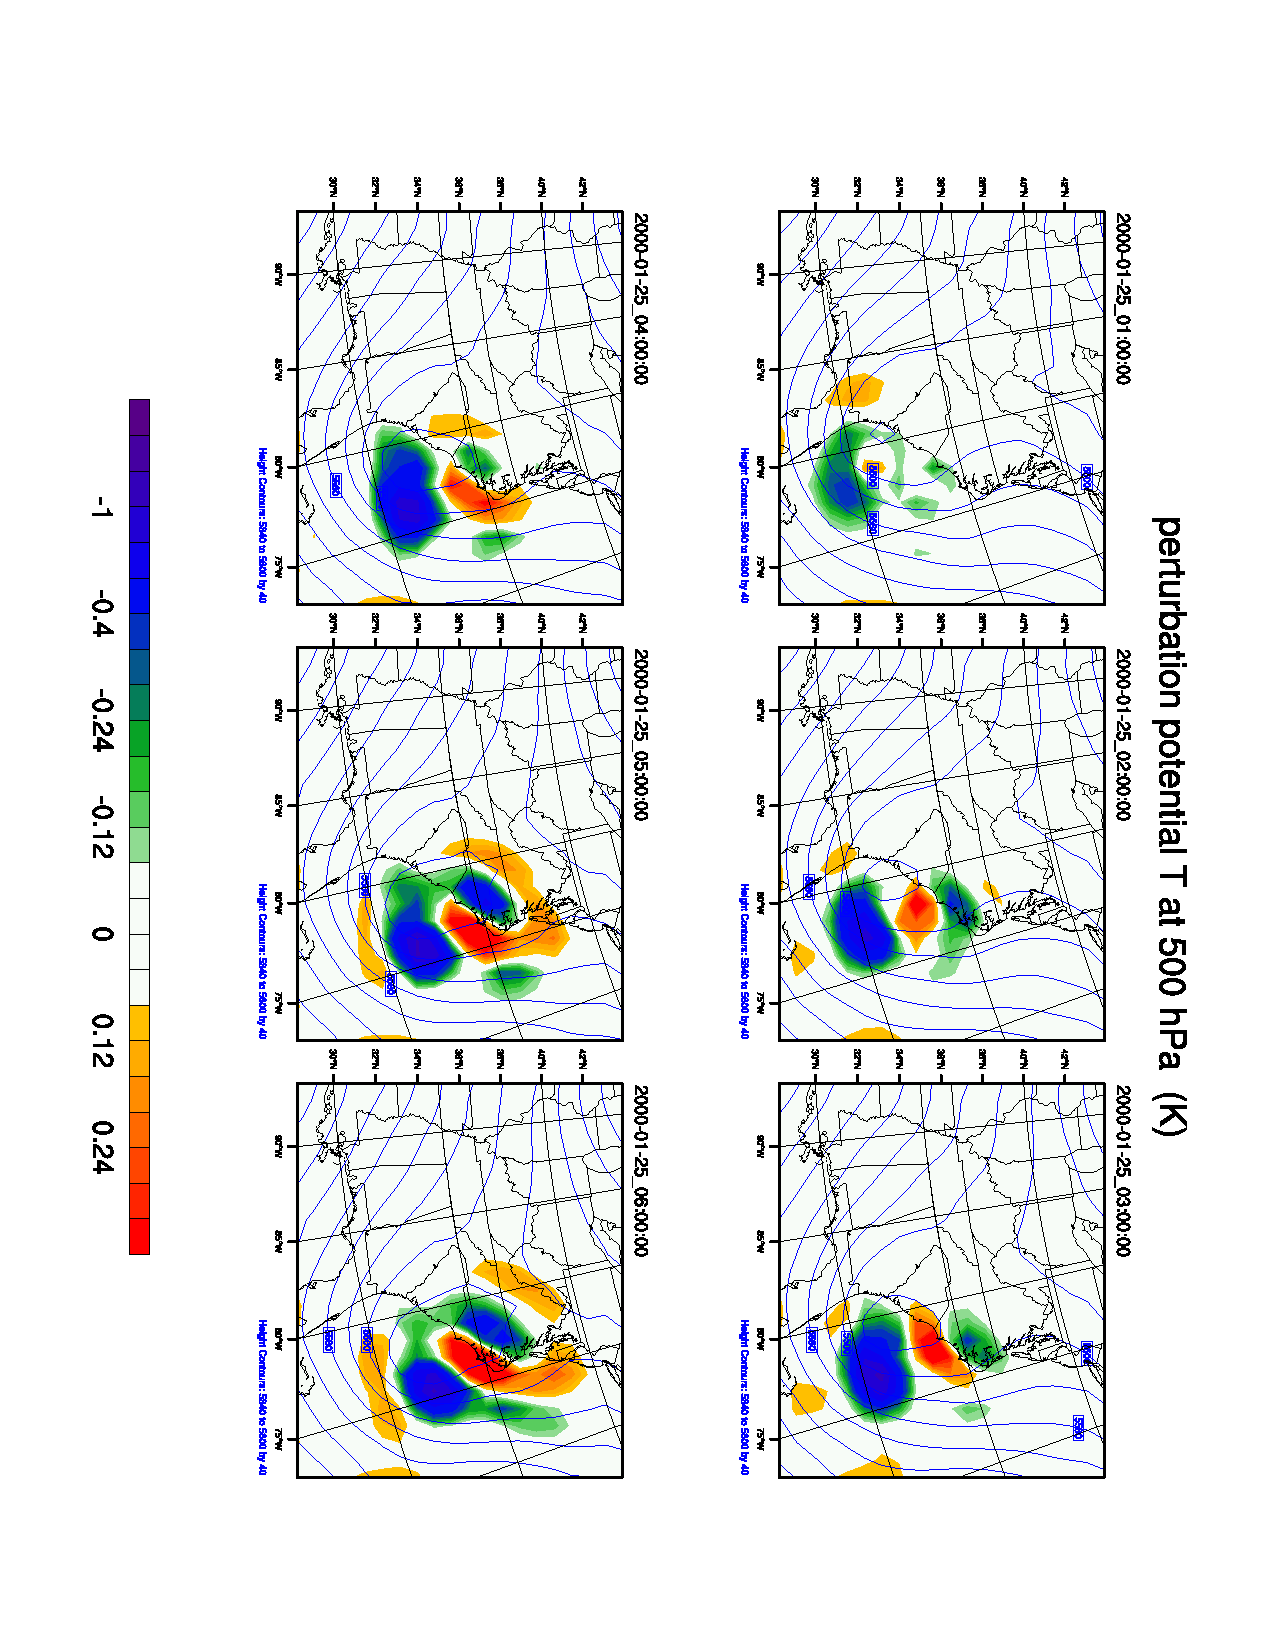
\includegraphics[trim=363 291 66 295, clip=true, angle=90, width=0.7\textwidth]{figures/center_lbc_6h} 
\end{figure} 
\end{frame}

\begin{frame}
\frametitle{500hPa $\theta$ increments from 0--6 h with LBC control}
\begin{figure} 
\centering 
\centering 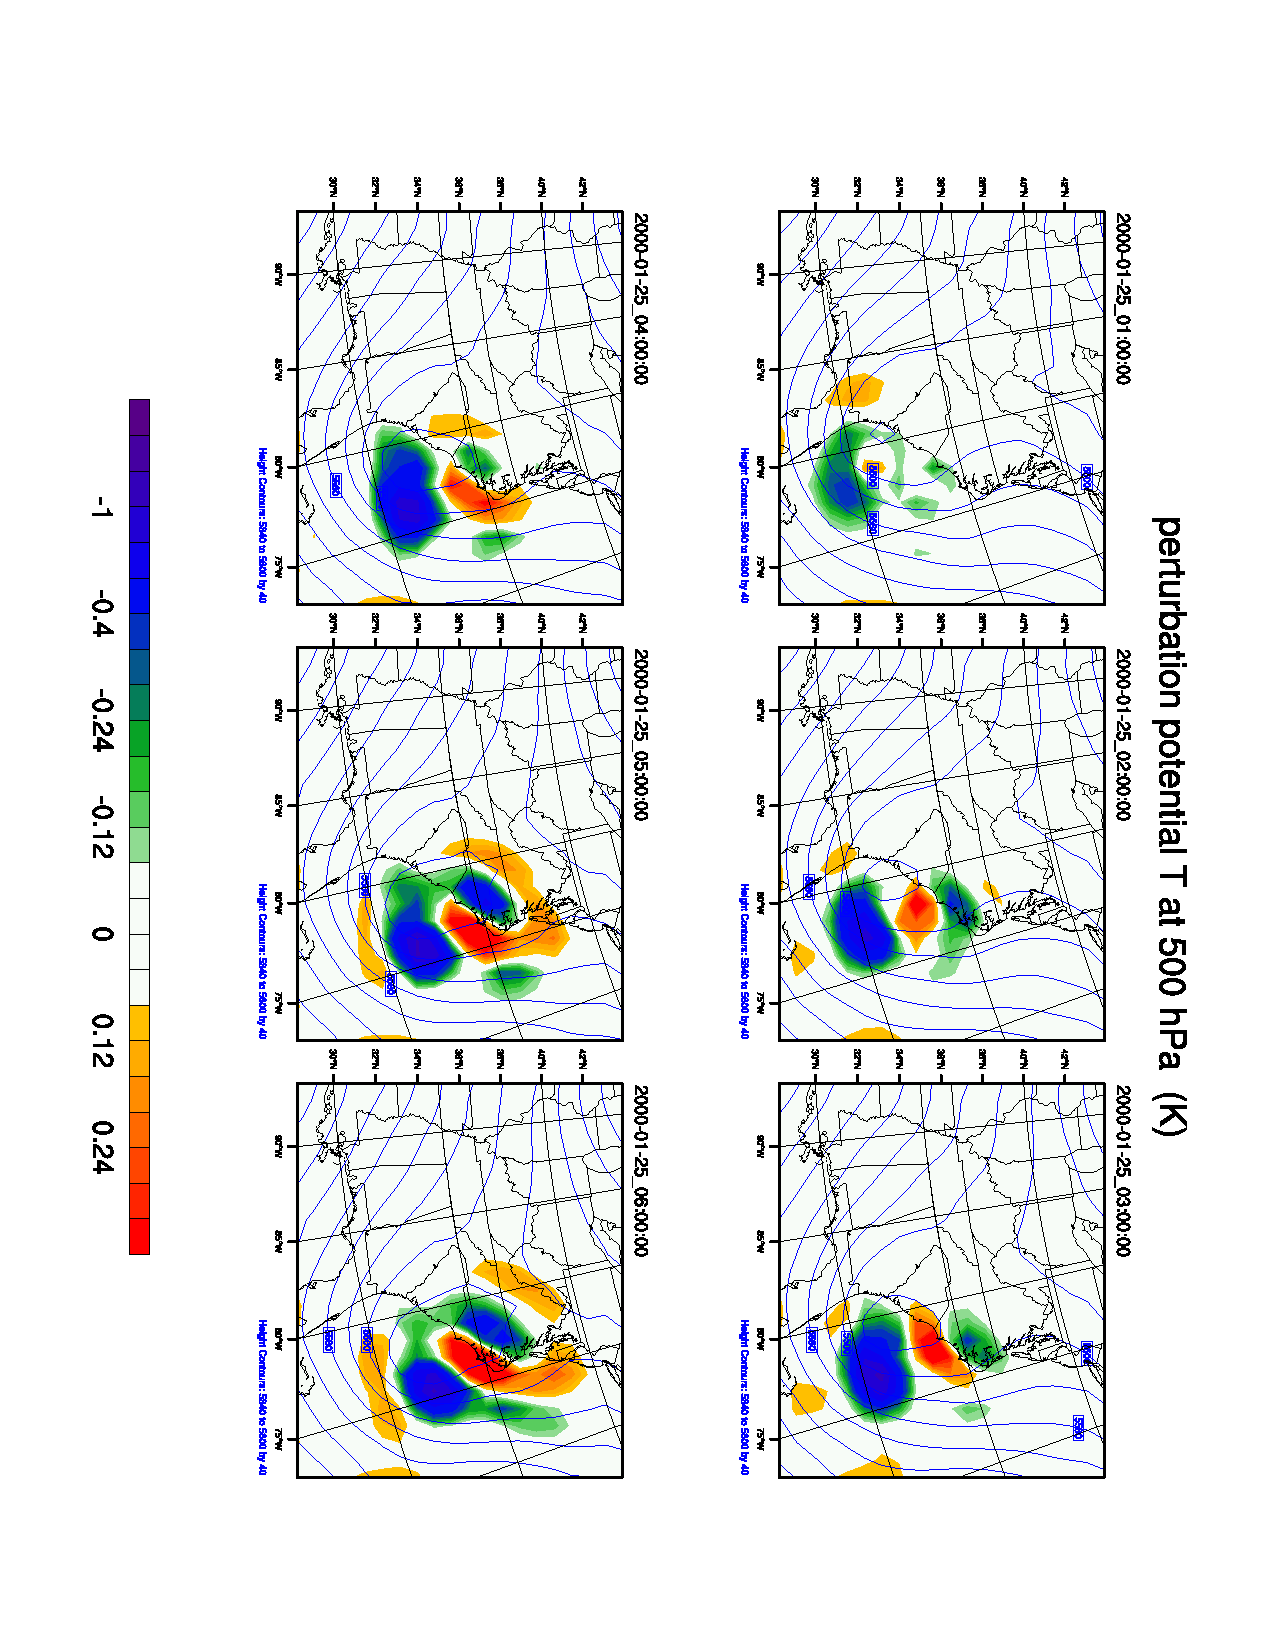
\includegraphics[trim=363 82 66 502, clip=true, angle=90, width=0.7\textwidth]{figures/center_lbc_6h} 
\end{figure} 
\end{frame}

\begin{frame}
\frametitle{500hPa $\theta$ increments from 0--6 h with LBC control}
\begin{figure} 
\centering 
\centering 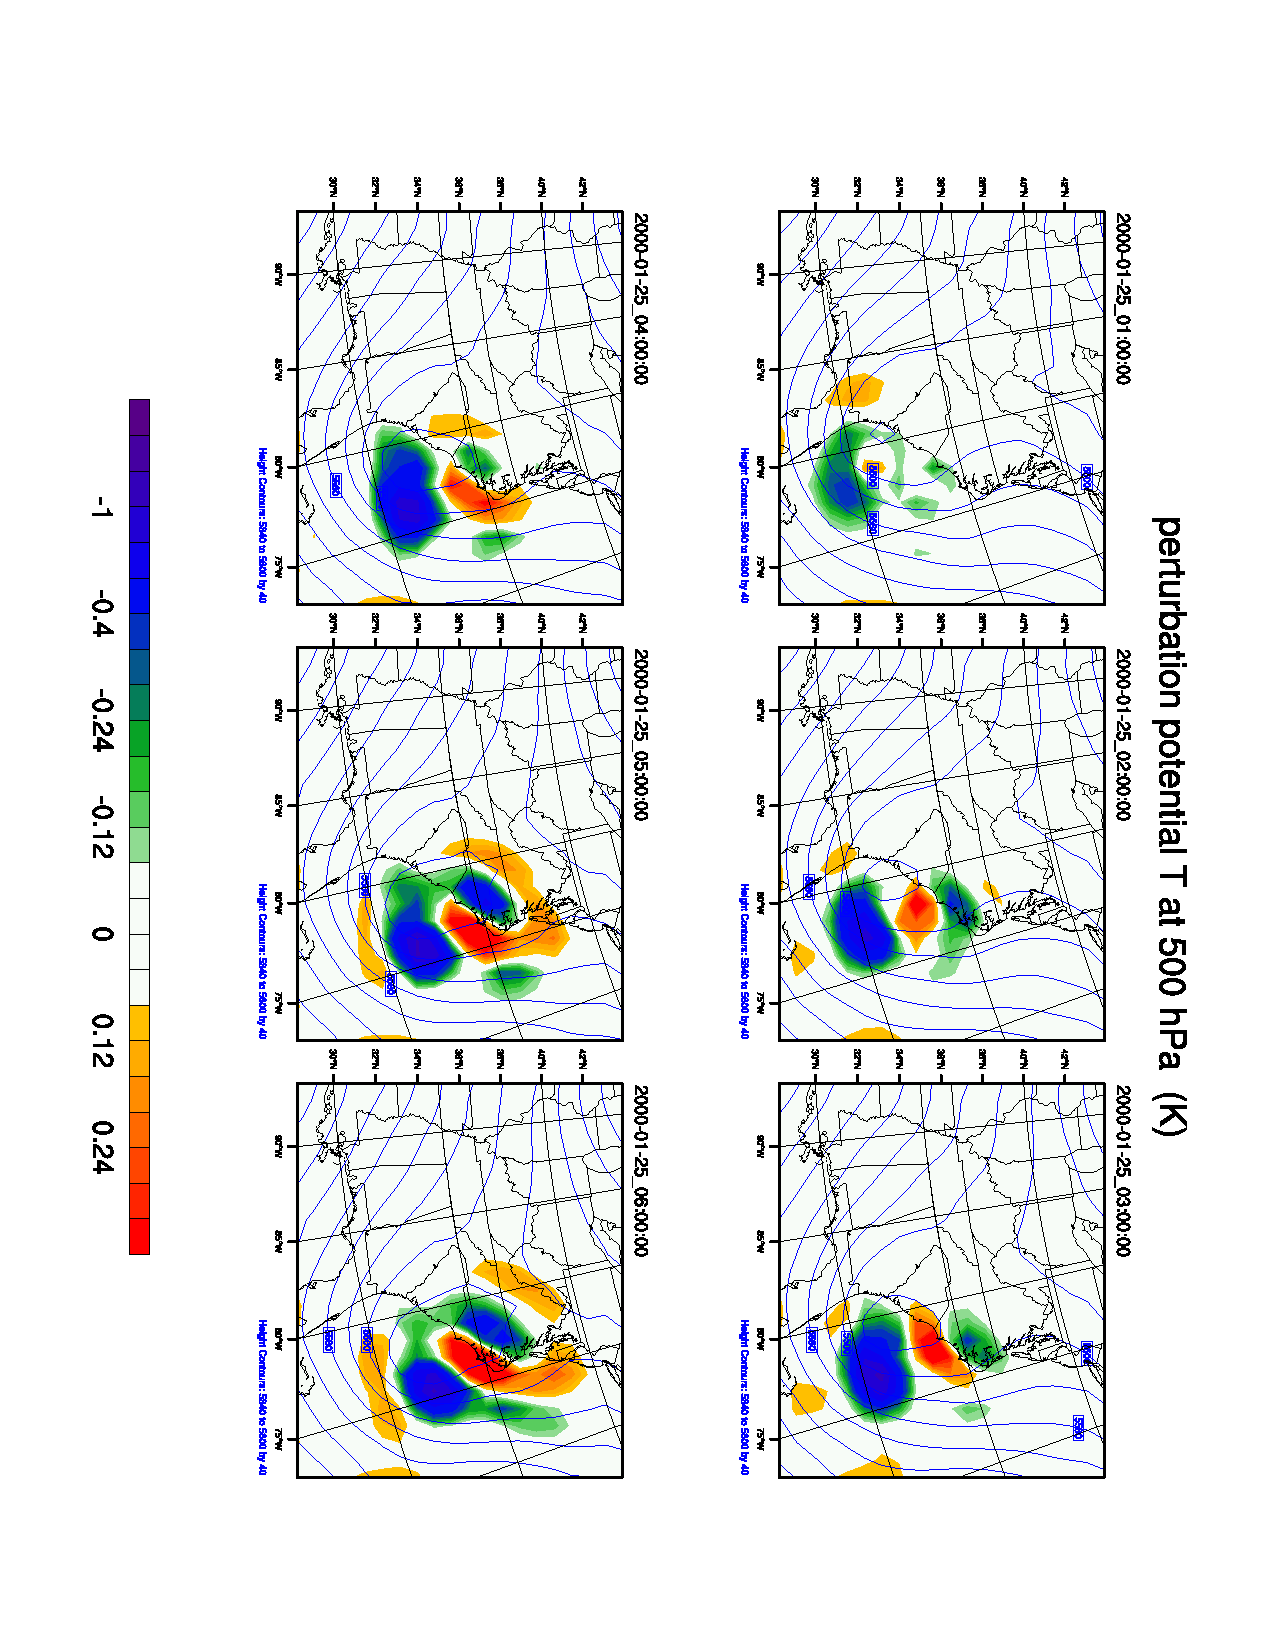
\includegraphics[trim=132 500 300 85, clip=true, angle=90, width=0.7\textwidth]{figures/center_lbc_6h} 
\end{figure} 
\end{frame}

\begin{frame}
\frametitle{500hPa $\theta$ increments from 0--6 h with LBC control}
\begin{figure} 
\centering 
\centering 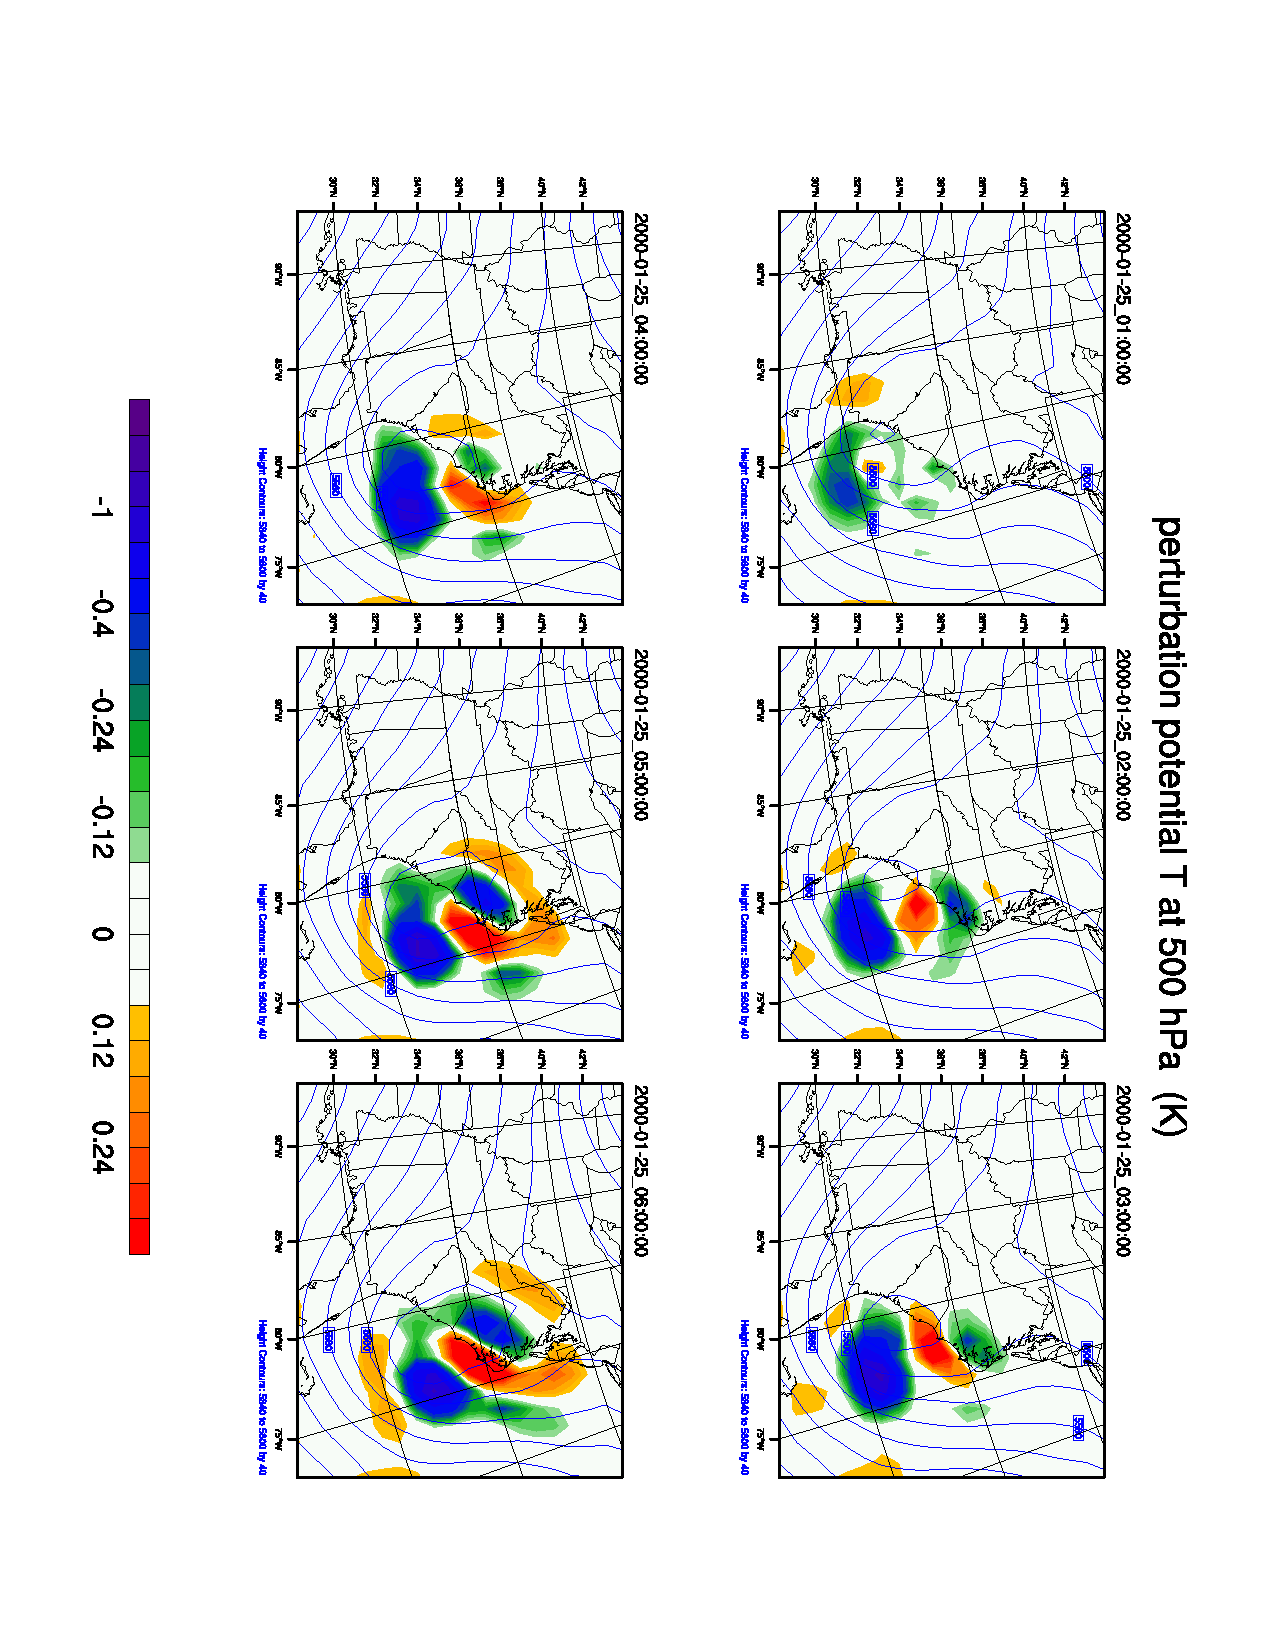
\includegraphics[trim=132 291 300 293, clip=true, angle=90, width=0.7\textwidth]{figures/center_lbc_6h} 
\end{figure} 
\end{frame}

\begin{frame}
\frametitle{500hPa $\theta$ increments from 0--6 h with LBC control}
\begin{figure} 
\centering 
\centering 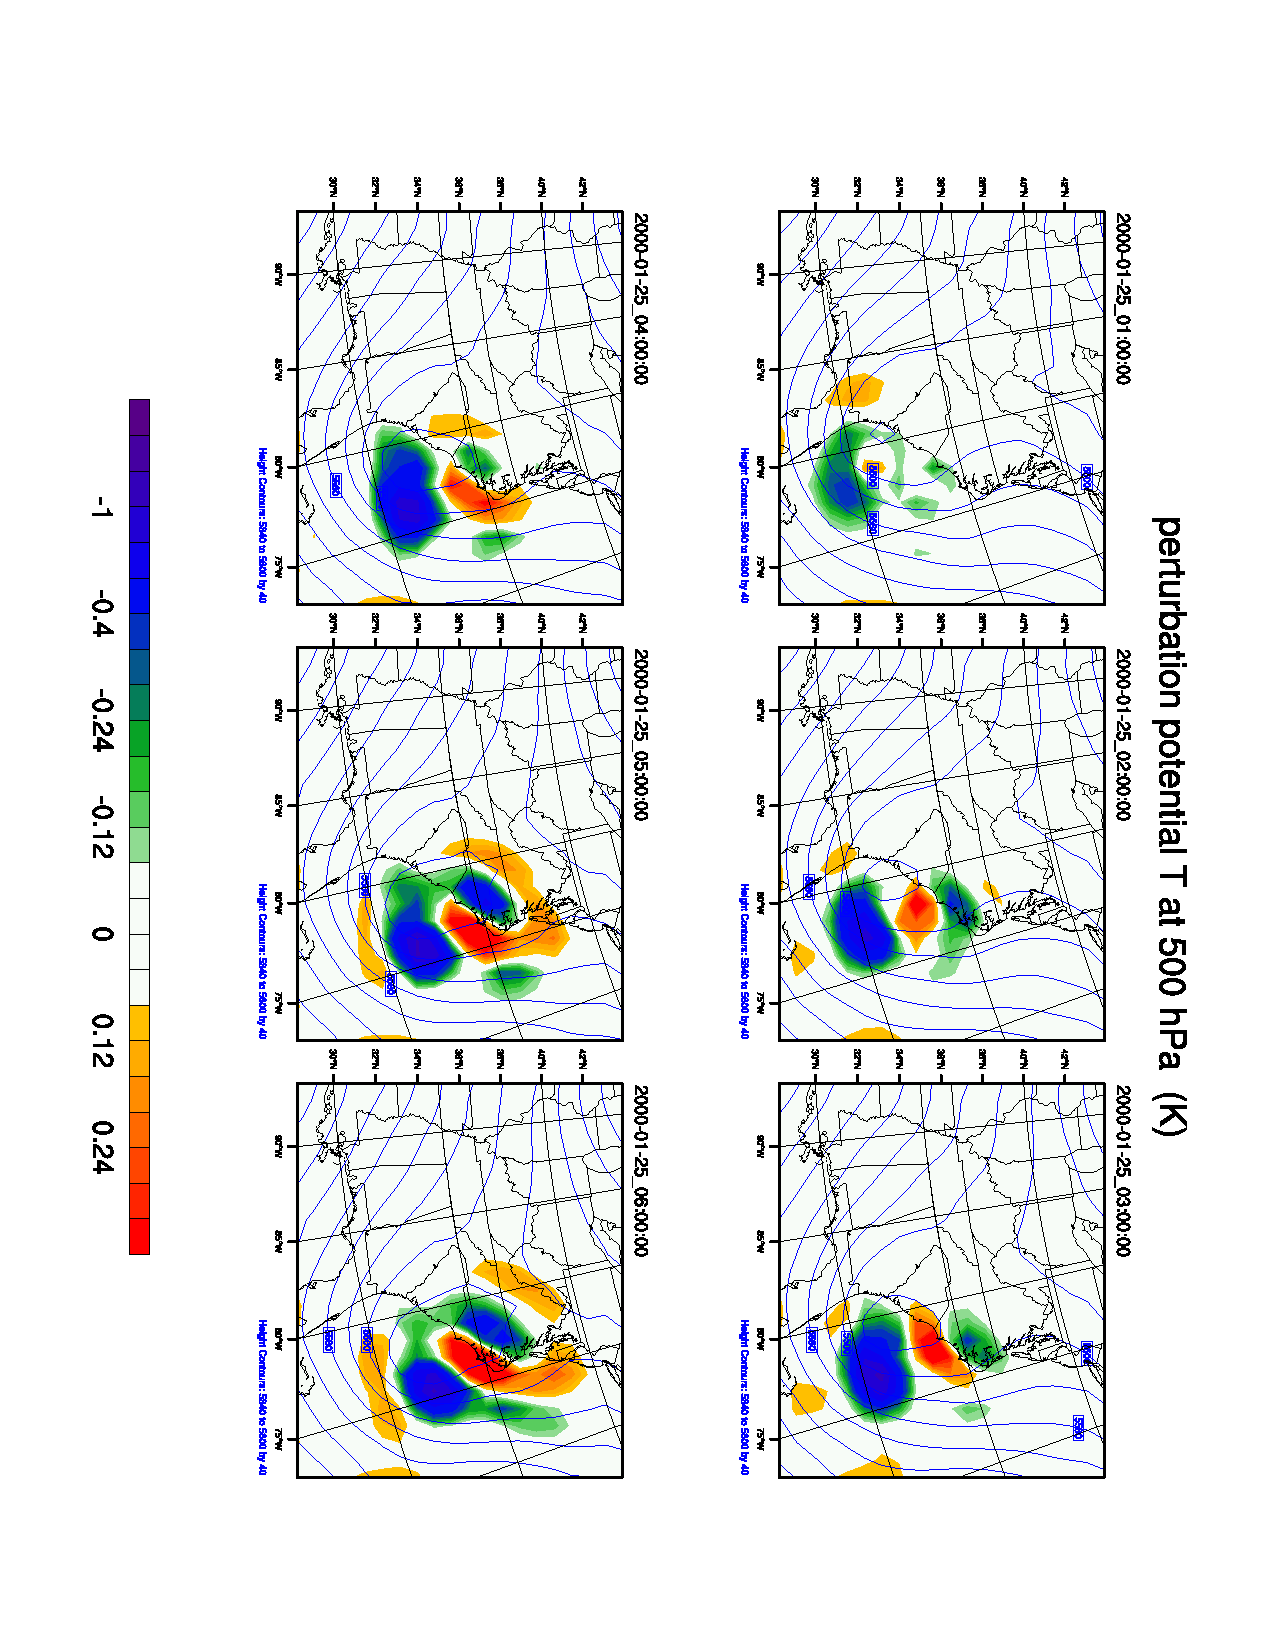
\includegraphics[trim=132 82 300 502, clip=true, angle=90, width=0.7\textwidth]{figures/center_lbc_6h} 
\end{figure} 
\end{frame}

\begin{frame}
\frametitle{Remark}
\begin{itemize}
\item The Final $J_{lbc}$ is increased from 0 to 0.01 \pause
\vspace{2mm}
%\item LBC control has some impact on the initial $\theta$ perturbation since it close to the boundary relaxation zone \pause
% Compared the figures w/ and w/o LBC control, the perturbation evolutions are almost the same, which implies that
\item  The LBC control doesn't change the minimization too much if the observation is far away from lateral boundary and out of the reach of the LBC influence during the assimilation window
\end{itemize}
\end{frame}

\end{comment}

\subsection{A 6 h observation close to boundary ($\Delta T= -0.95K$)}

\begin{frame}
\frametitle{500hPa $\theta$ analysis increments at 0 h}
$\color{red}\textbf{+}$ is the location of the observation at 6h
\begin{columns}[t]
	\begin{column}{6cm}
		\begin{figure}
			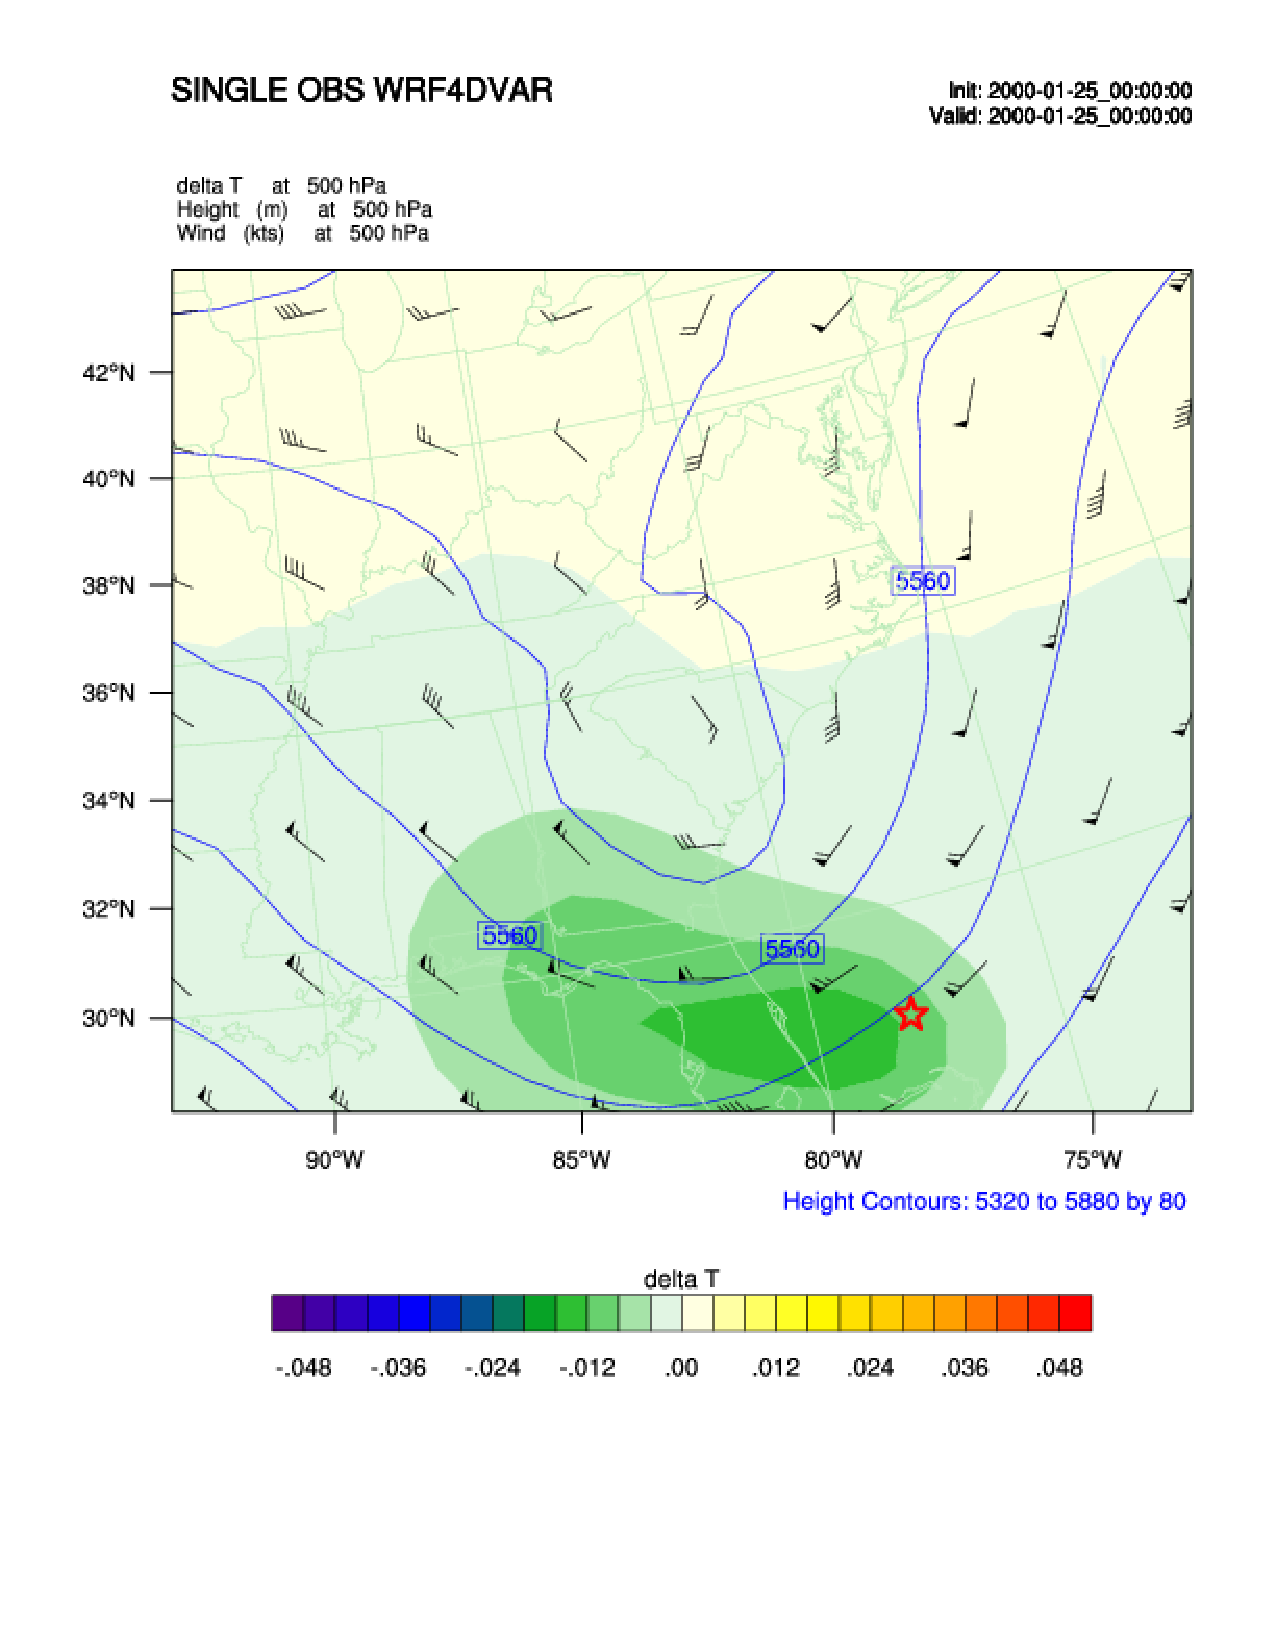
\includegraphics[trim=0 100 0 120, clip=true, width=0.90\textwidth]{figures/boundary}
			\caption {w/o LBC control}
		\end{figure}
	\end{column}
	\begin{column}{6cm}
		\begin{figure}
			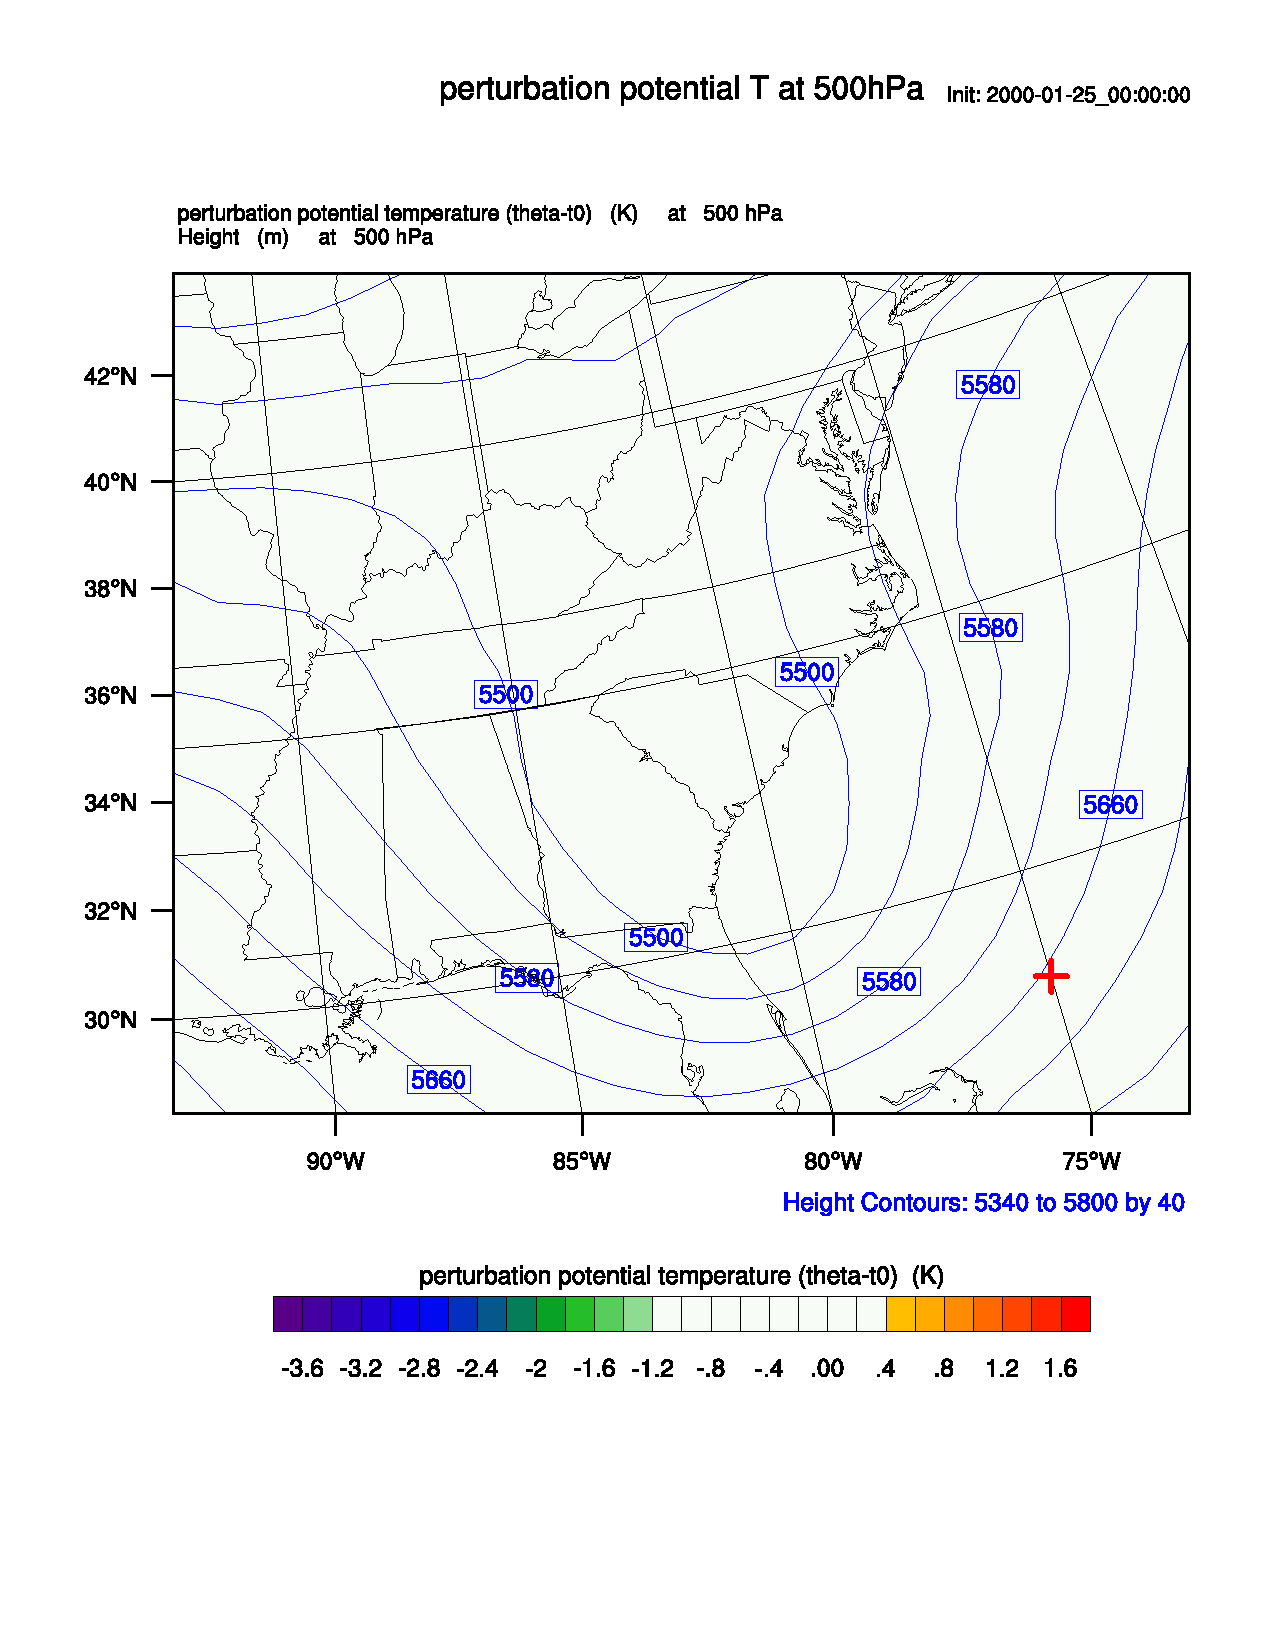
\includegraphics[trim=0 100 0 120, clip=true, width=0.90\textwidth]{figures/boundary_lbc}
			\caption {with LBC control}
		\end{figure}
	\end{column}
\end{columns}
\end{frame}

\begin{frame}
\frametitle{500hPa $\theta$ increments at {\color{red}00h} with LBC control}
\begin{figure} 
\centering 
\centering 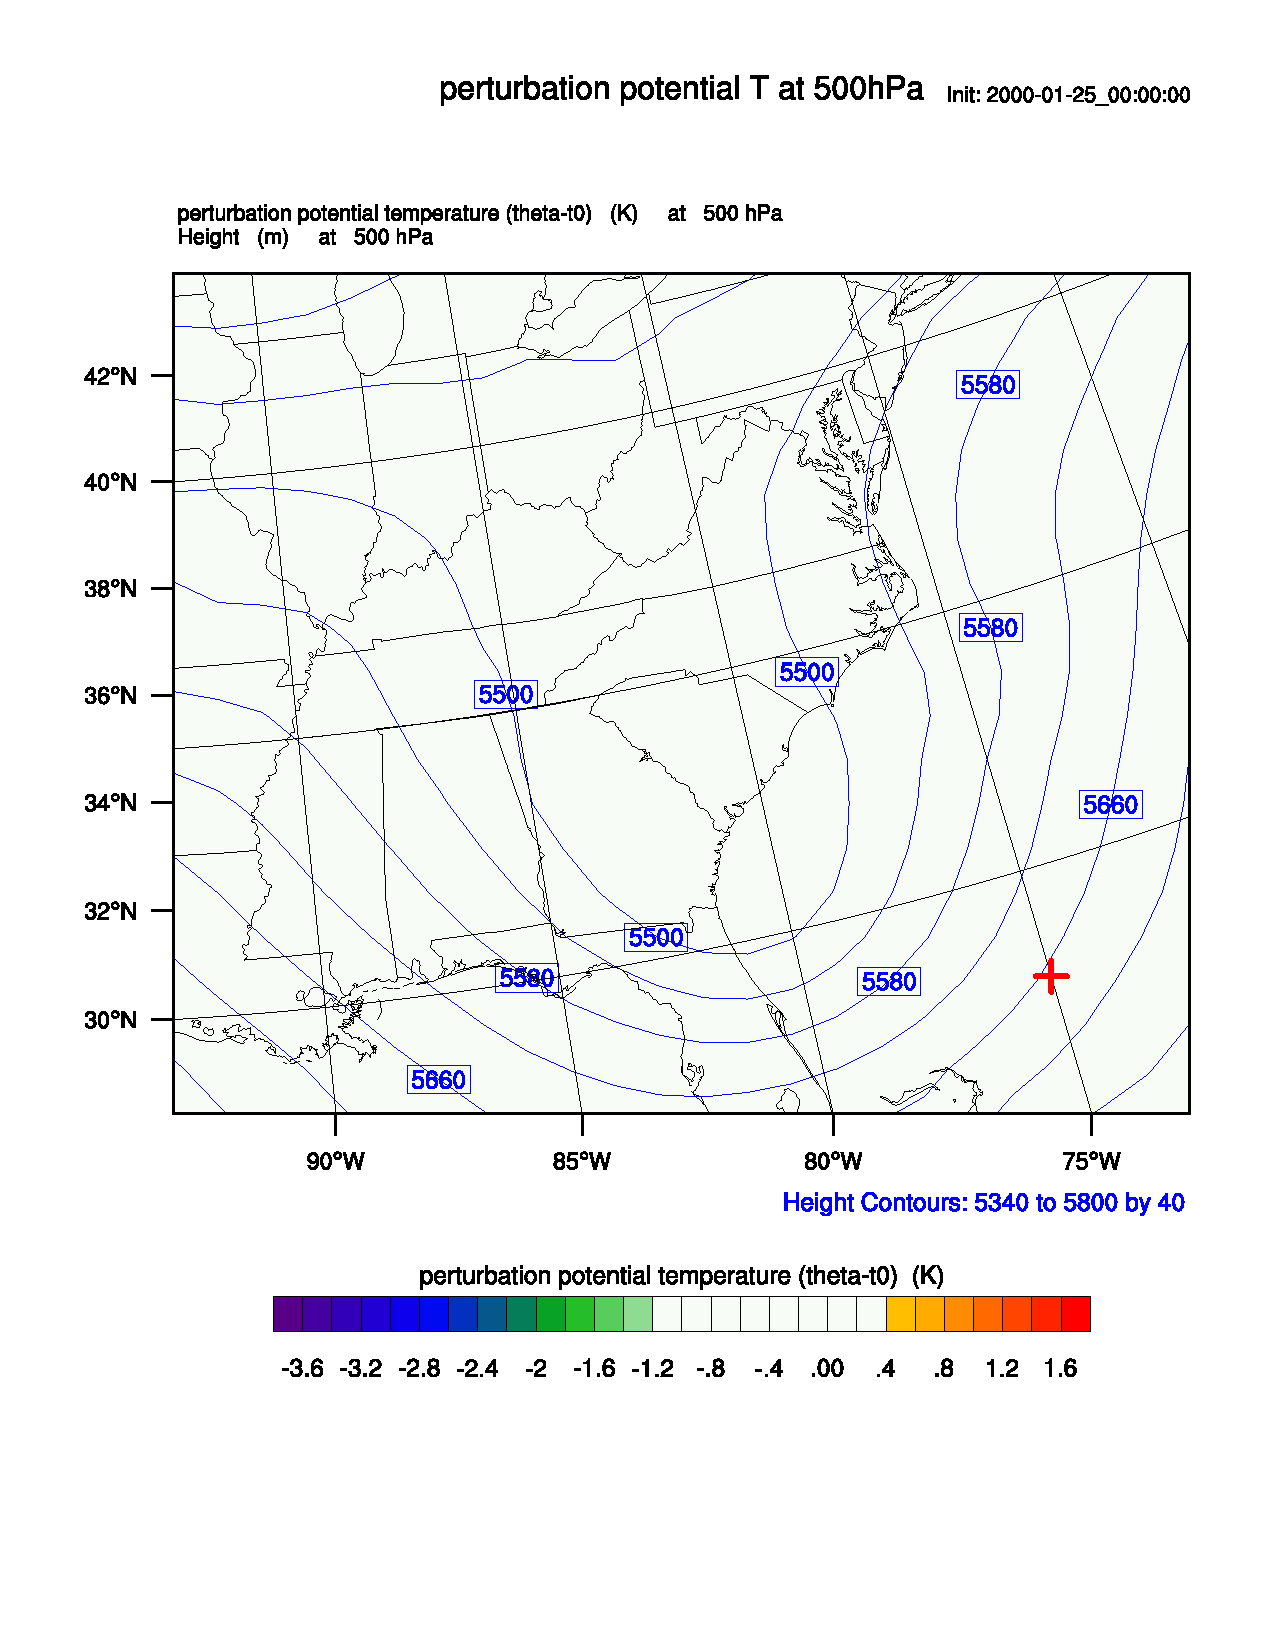
\includegraphics[width=0.6\textwidth]{figures/boundary_lbc} 
\end{figure} 
\end{frame}

\begin{frame}
\frametitle{500hPa $\theta$ increments at {\color{red}01h} with LBC control}
\begin{figure} 
\centering 
\centering 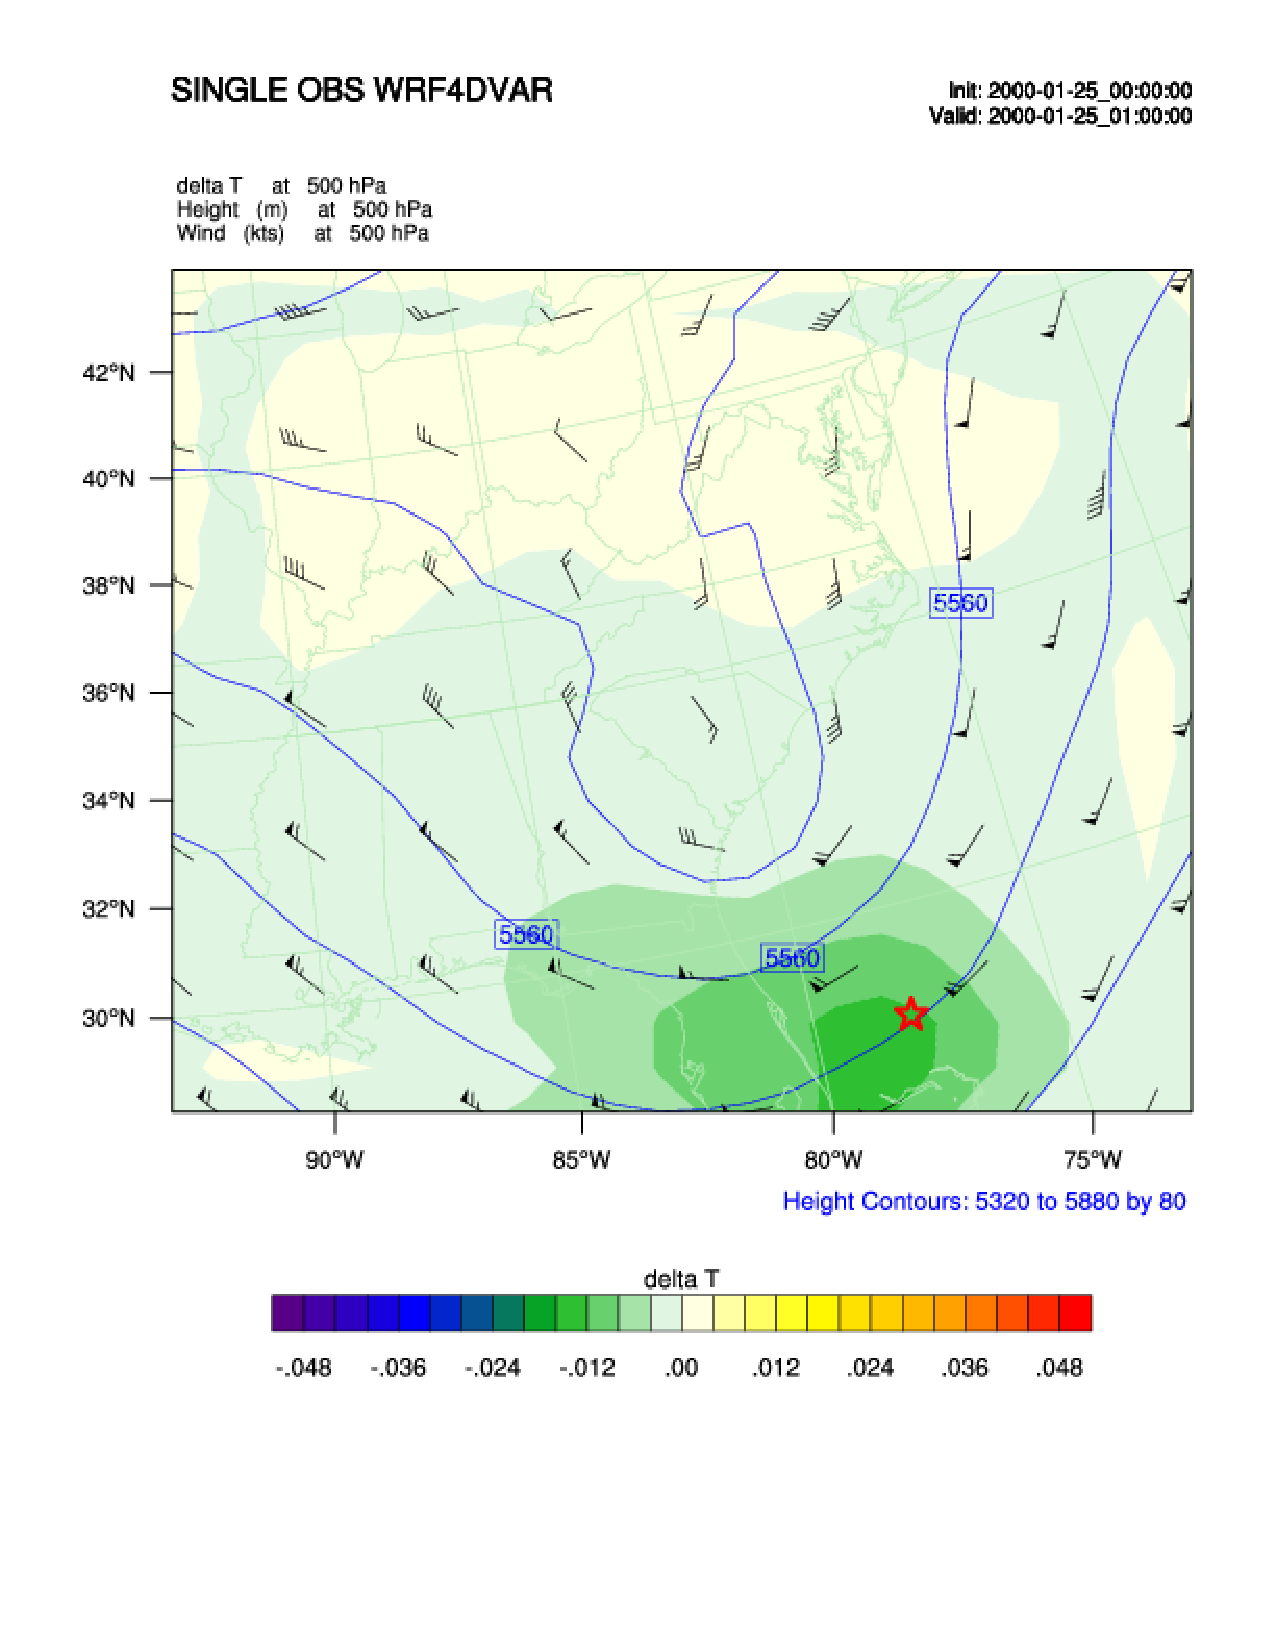
\includegraphics[width=0.6\textwidth]{figures/boundary_lbc_1h} 
\end{figure} 
\end{frame}

\begin{frame}
\frametitle{500hPa $\theta$ increments at {\color{red}02h} with LBC control}
\begin{figure} 
\centering 
\centering 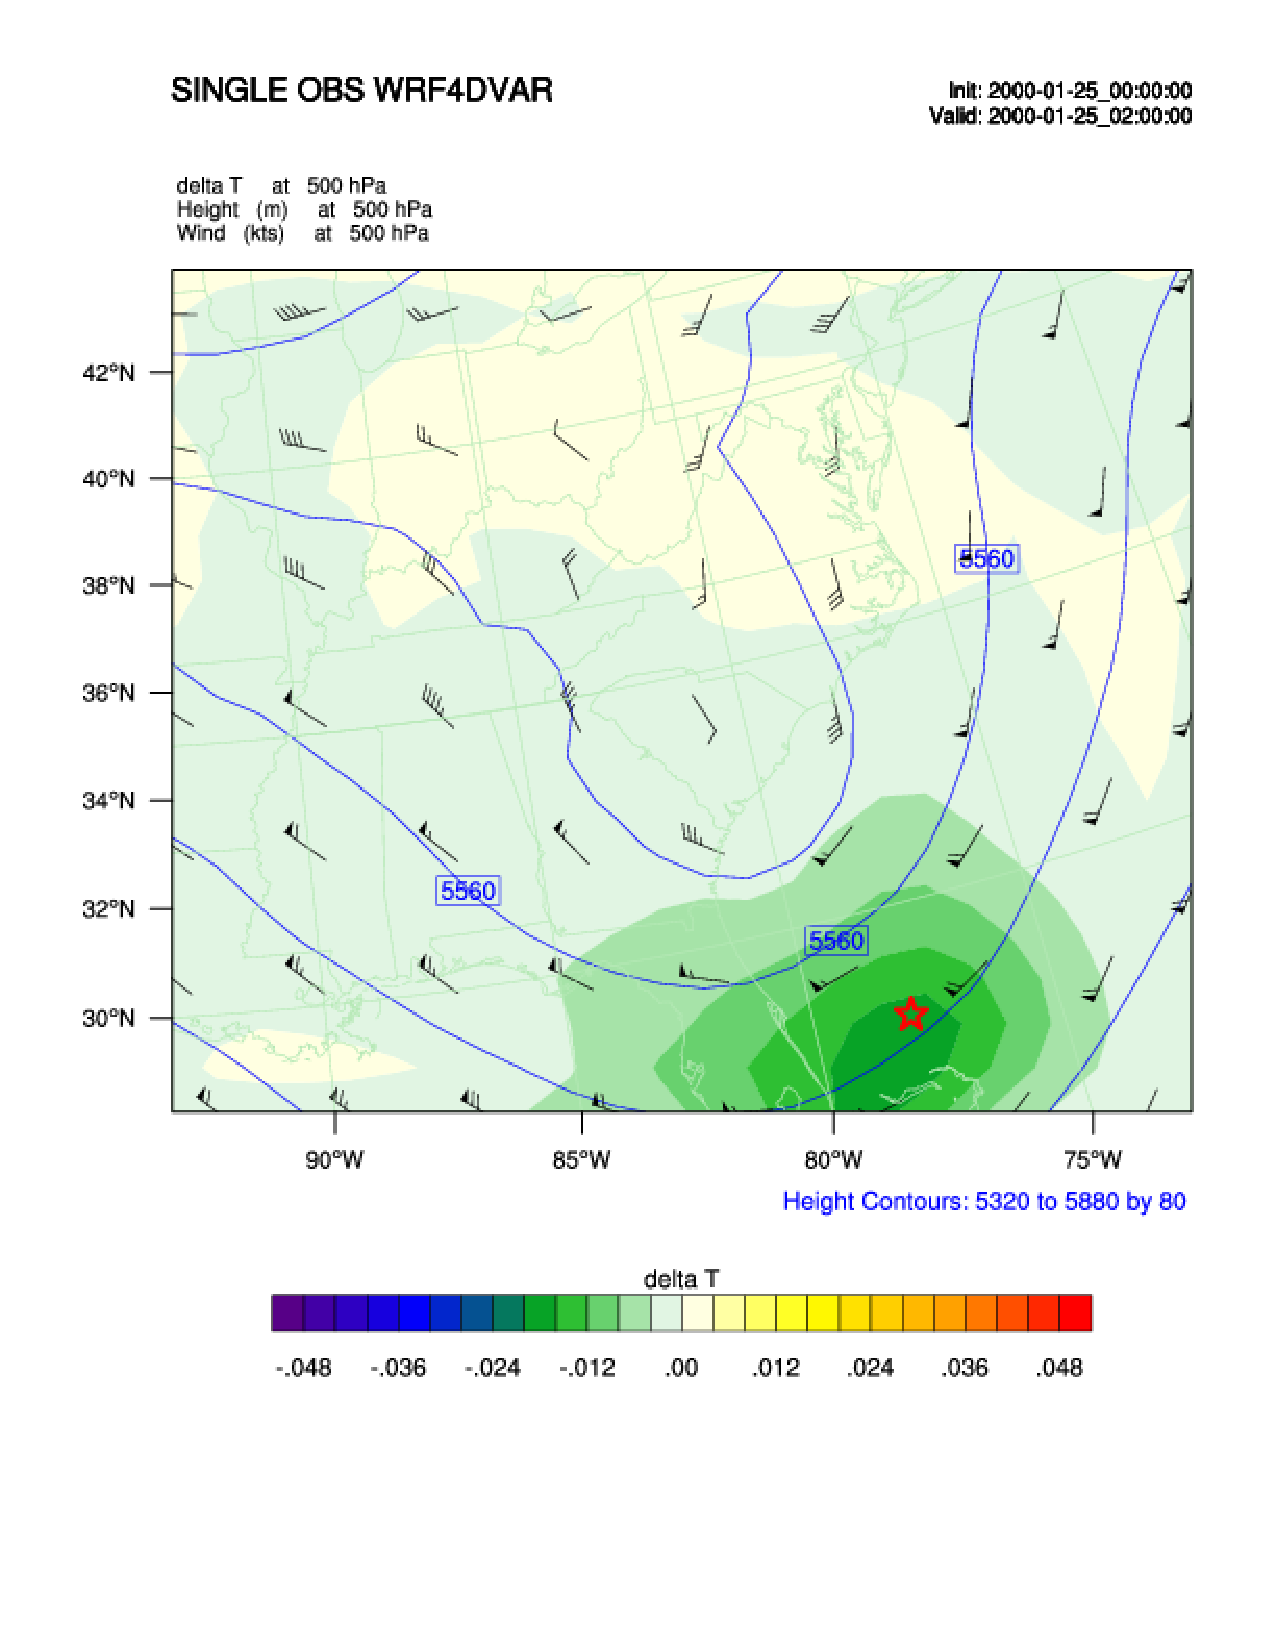
\includegraphics[width=0.6\textwidth]{figures/boundary_lbc_2h} 
\end{figure} 
\end{frame}

\begin{frame}
\frametitle{500hPa $\theta$ increments at {\color{red}03h} with LBC control}
\begin{figure} 
\centering 
\centering 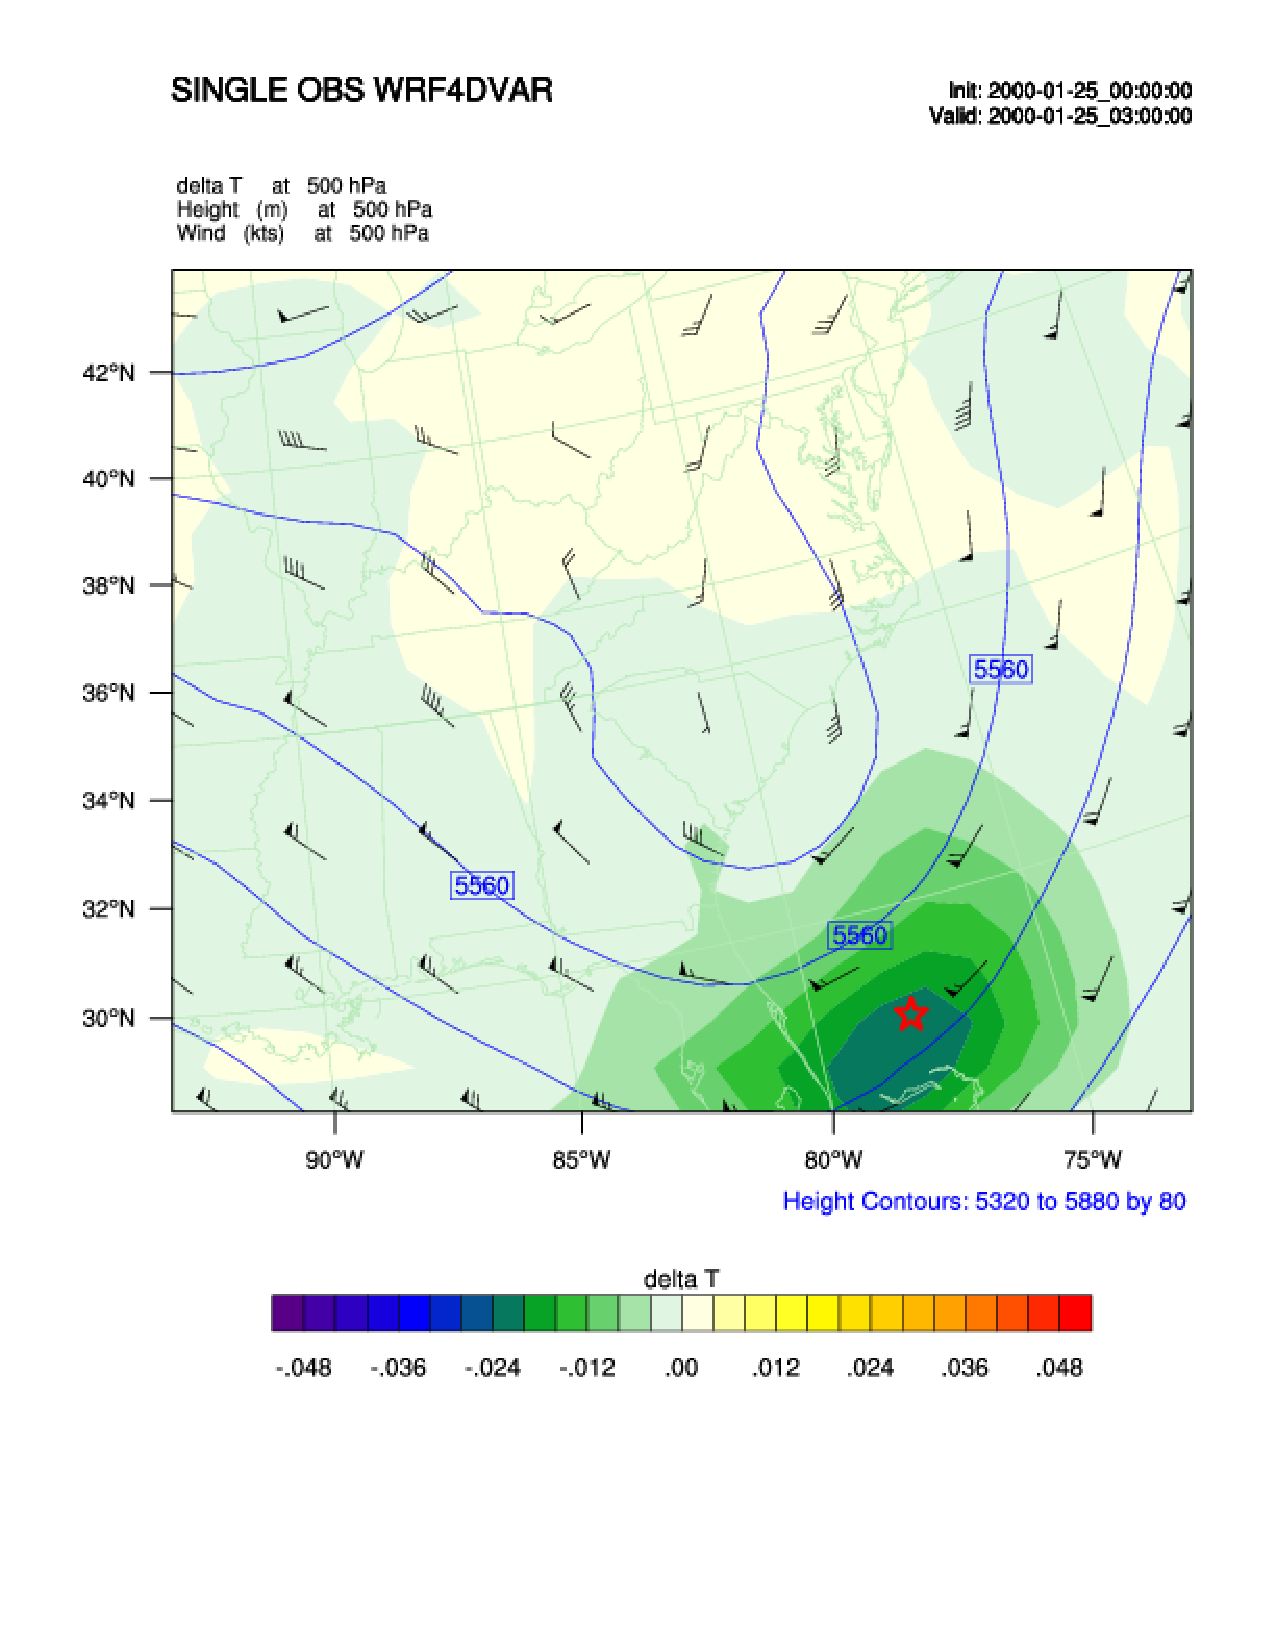
\includegraphics[width=0.6\textwidth]{figures/boundary_lbc_3h} 
\end{figure} 
\end{frame}

\begin{frame}
\frametitle{500hPa $\theta$ increments at {\color{red}04h} with LBC control}
\begin{figure} 
\centering 
\centering 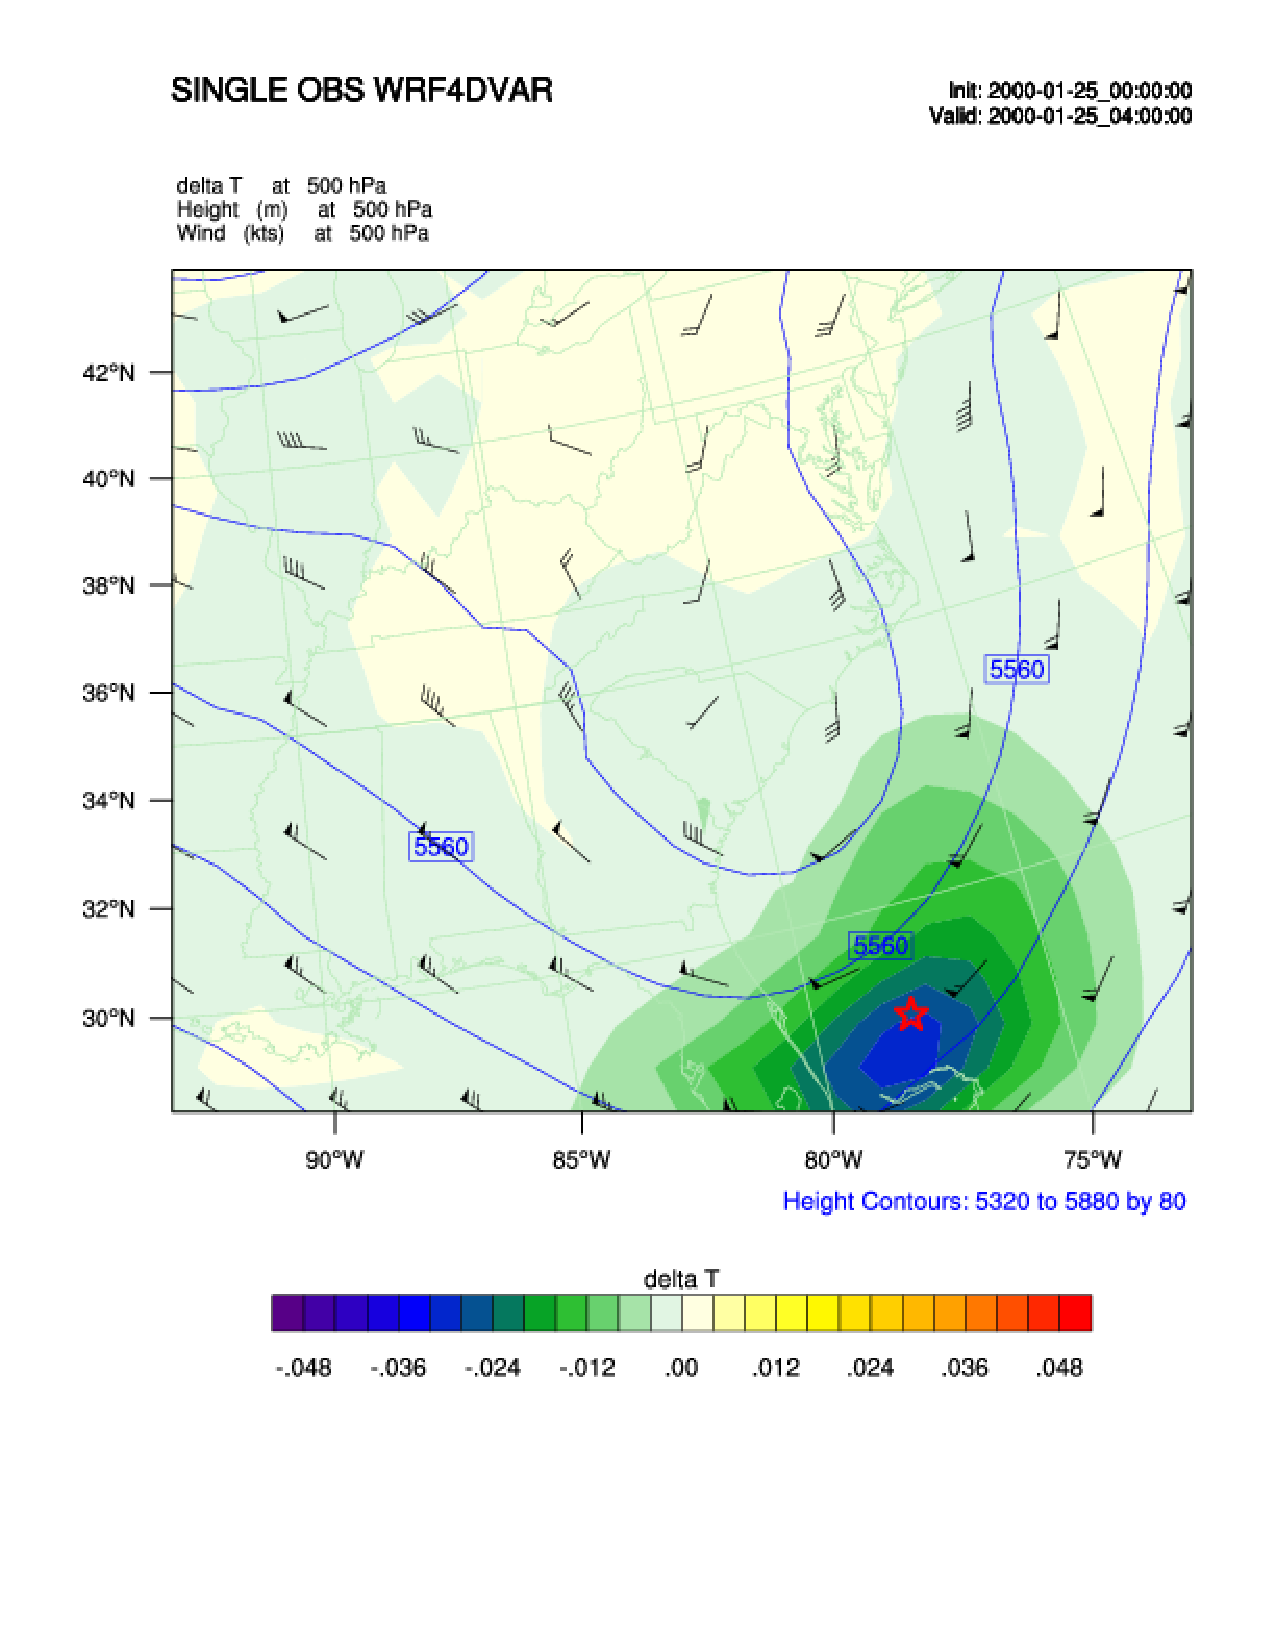
\includegraphics[width=0.6\textwidth]{figures/boundary_lbc_4h} 
\end{figure} 
\end{frame}

\begin{frame}
\frametitle{500hPa $\theta$ increments at {\color{red}05h} with LBC control}
\begin{figure} 
\centering 
\centering 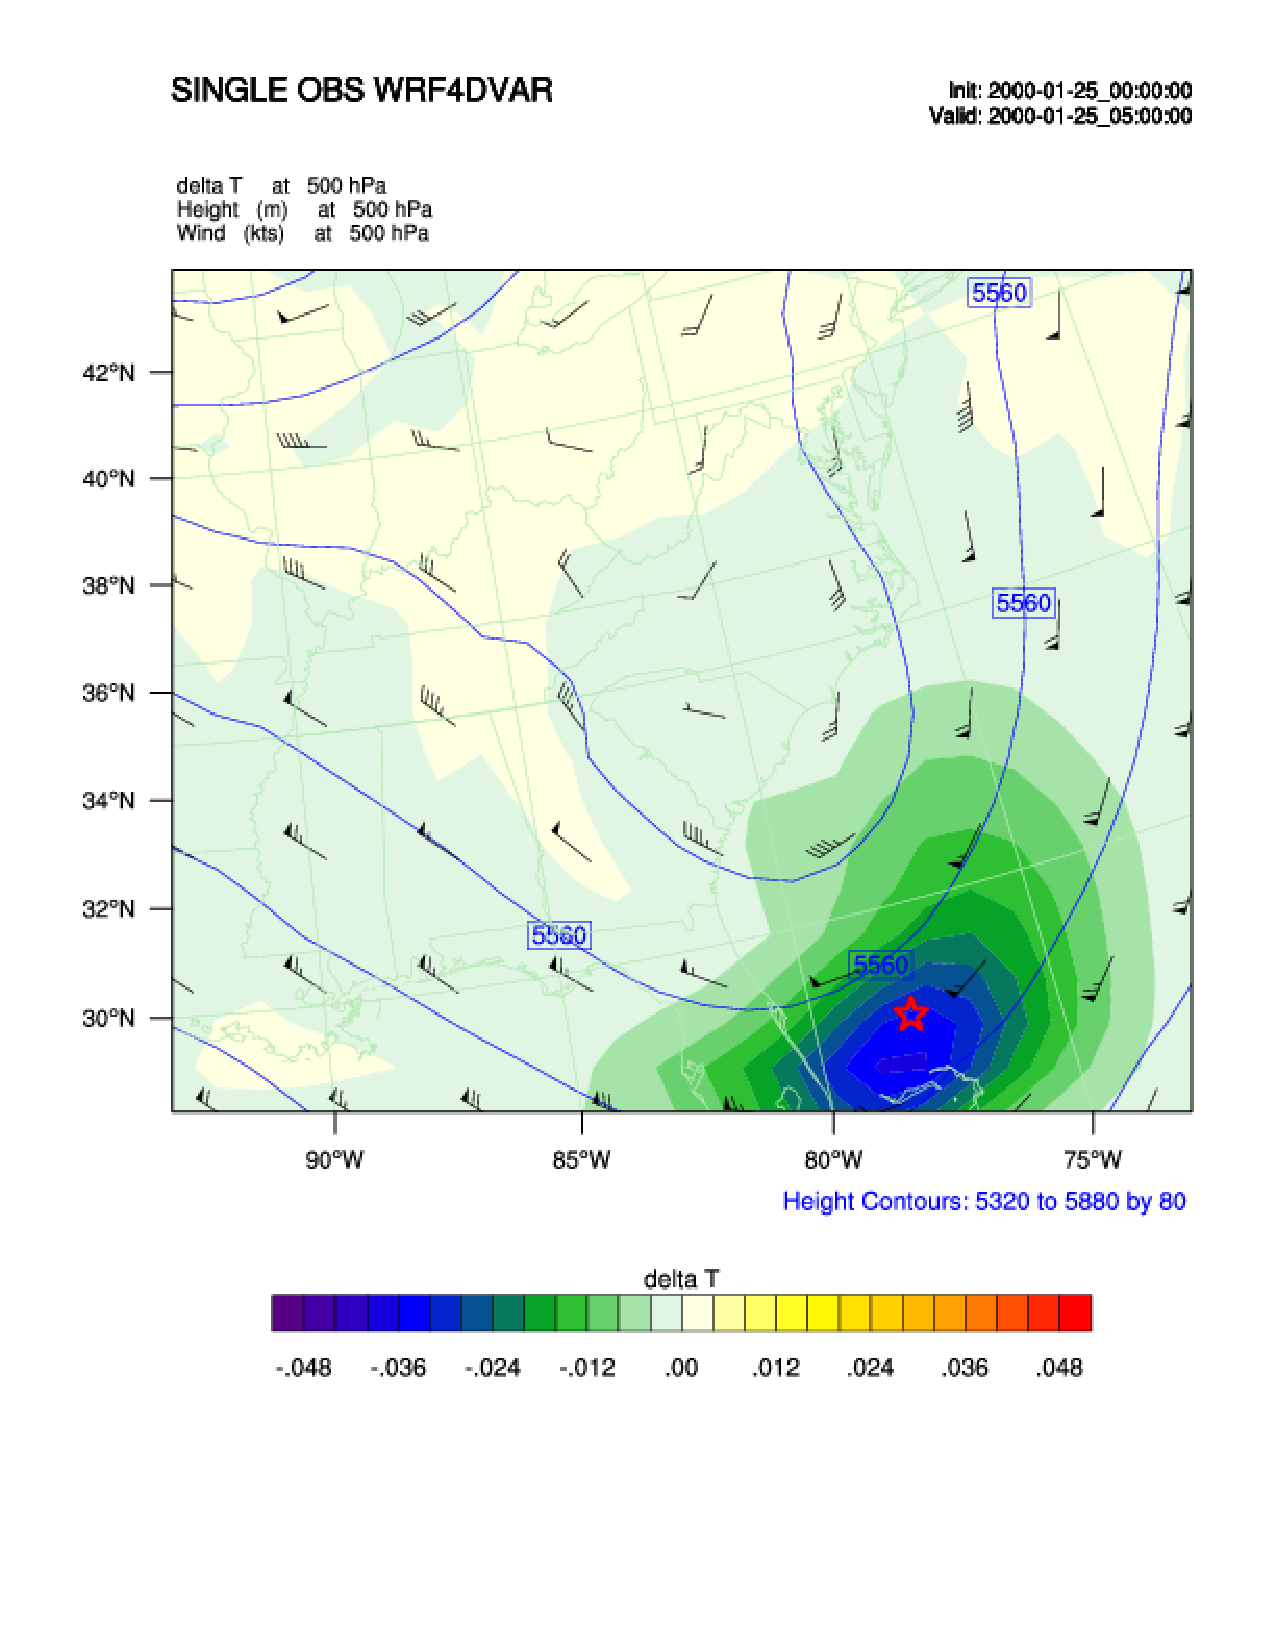
\includegraphics[width=0.6\textwidth]{figures/boundary_lbc_5h} 
\end{figure} 
\end{frame}

\begin{frame}
\frametitle{500hPa $\theta$ increments at {\color{red}06h} with LBC control}
\begin{figure} 
\centering 
\centering 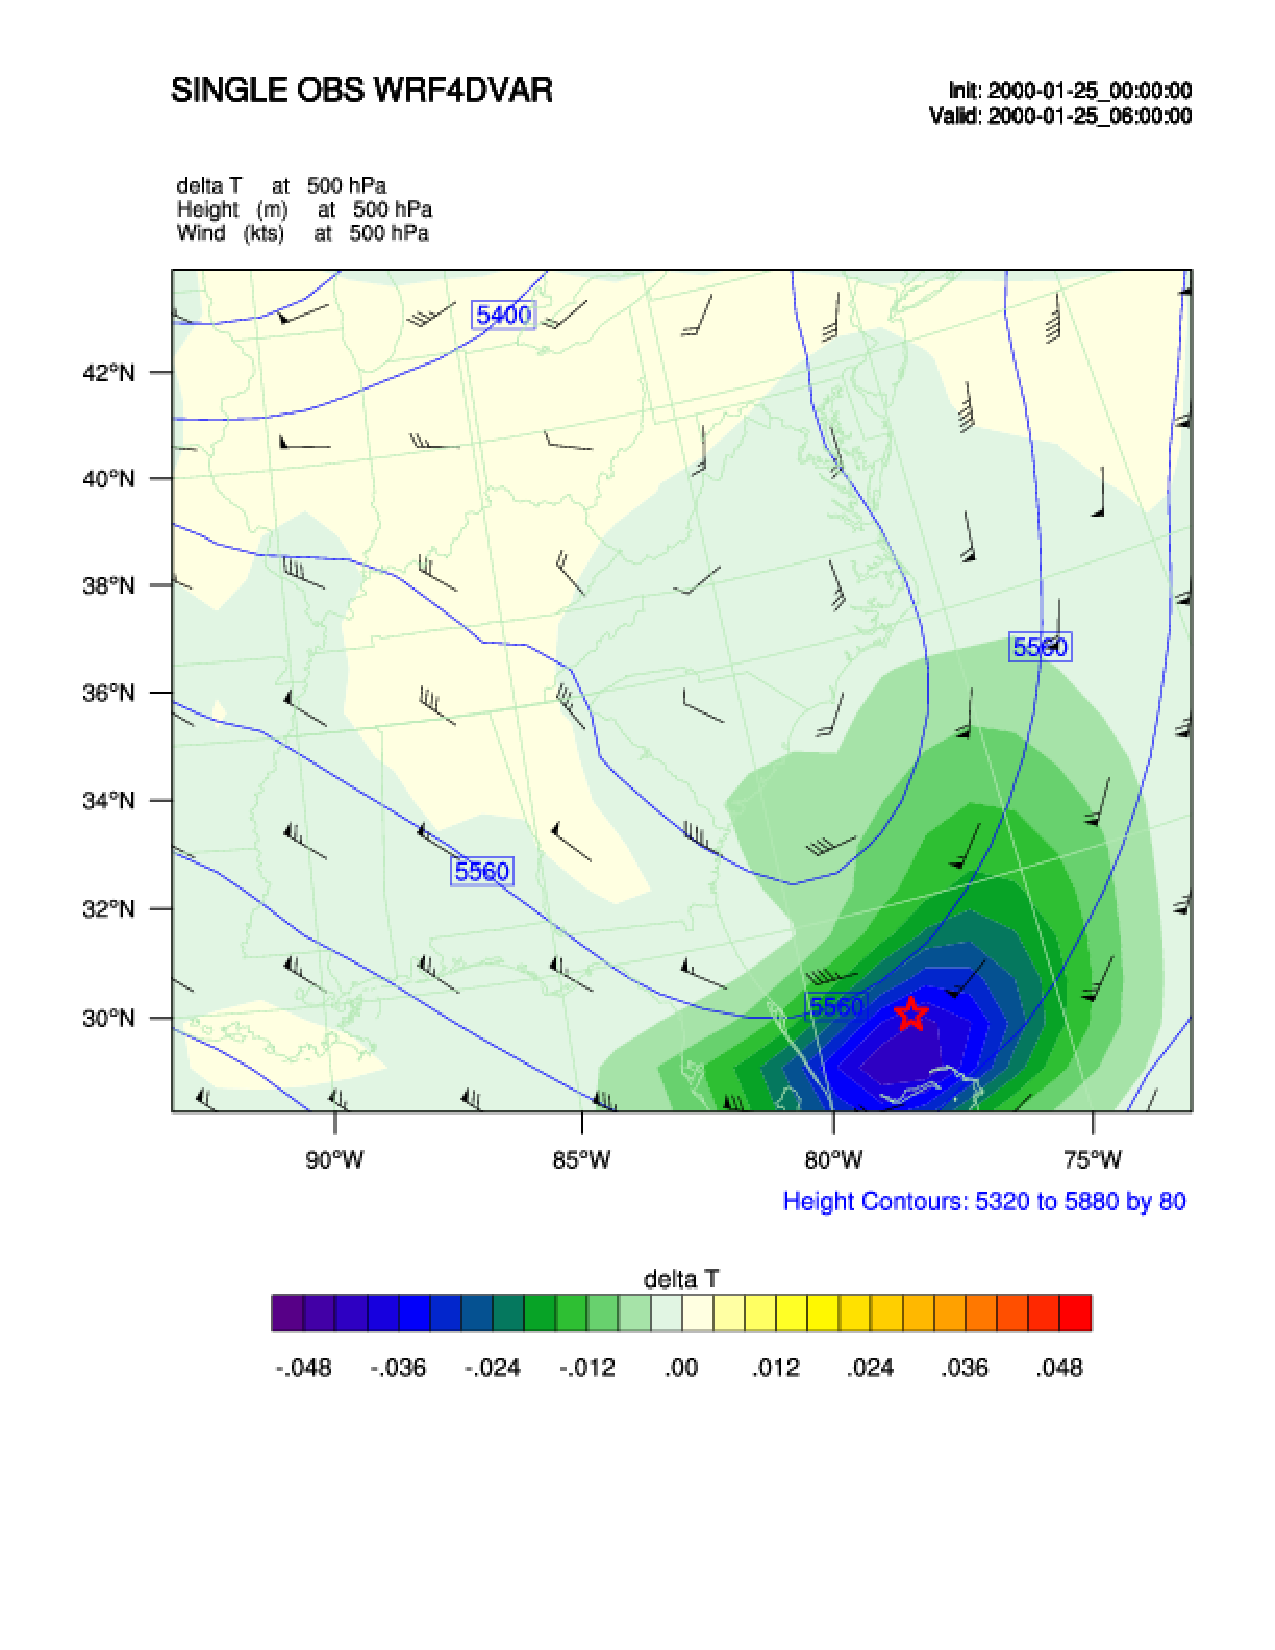
\includegraphics[width=0.6\textwidth]{figures/boundary_lbc_6h} 
\end{figure} 
\end{frame}

\begin{frame}
\begin{itemize}
\item Clearly flow-dependent increments is located upstream the observation in IC. \pause
\item The boundary conditions at both the start and end of the assimilation window are changed. \pause
\item The analysis increment of -0.48K at the observation location on 6h. \pause
\item The LBC contributes the information to propagate ! ?
\end{itemize}
\end{frame}

\begin{frame}
\frametitle{500hPa $\theta$ increments at {\color{red}00h} w/o LBC control}
\begin{figure} 
\centering 
\centering 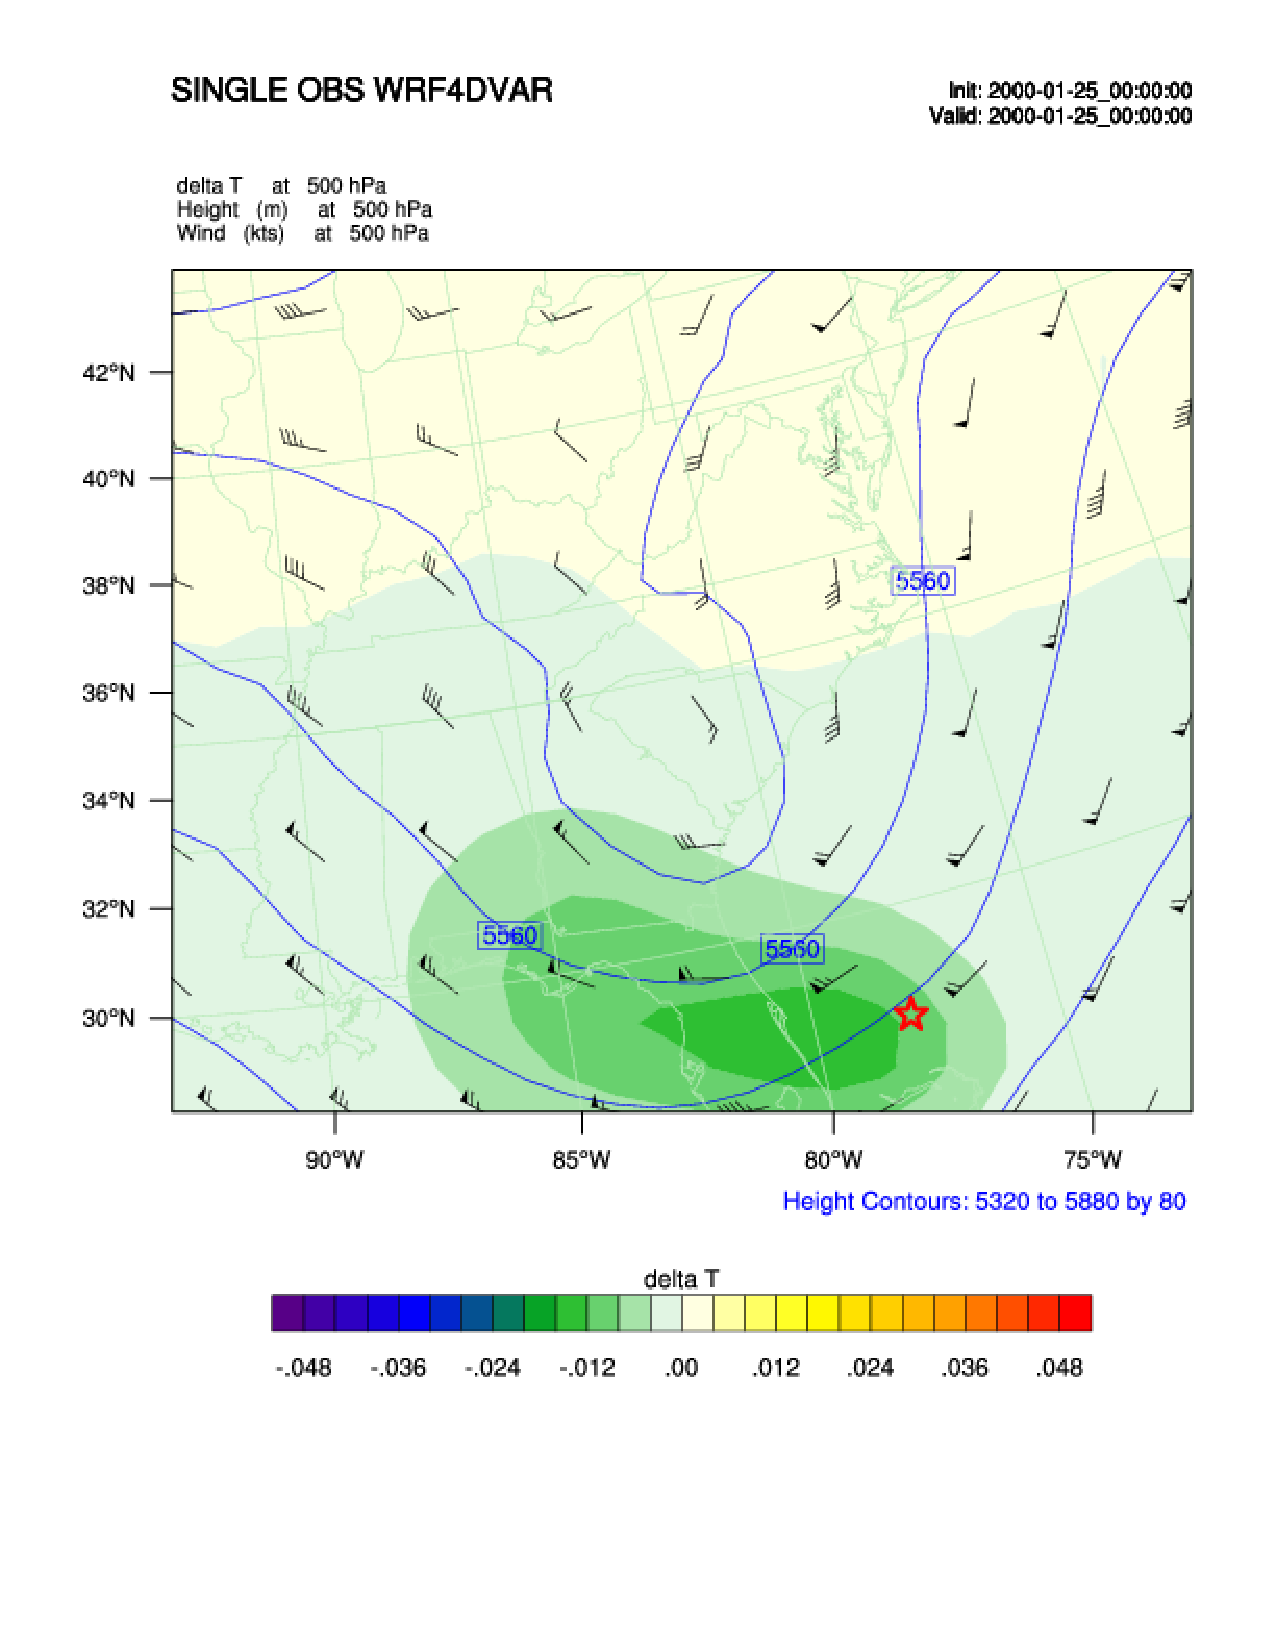
\includegraphics[width=0.6\textwidth]{figures/boundary} 
\end{figure} 
\end{frame}

\begin{frame}
\frametitle{500hPa $\theta$ increments at {\color{red}01h} w/o LBC control}
\begin{figure} 
\centering 
\centering 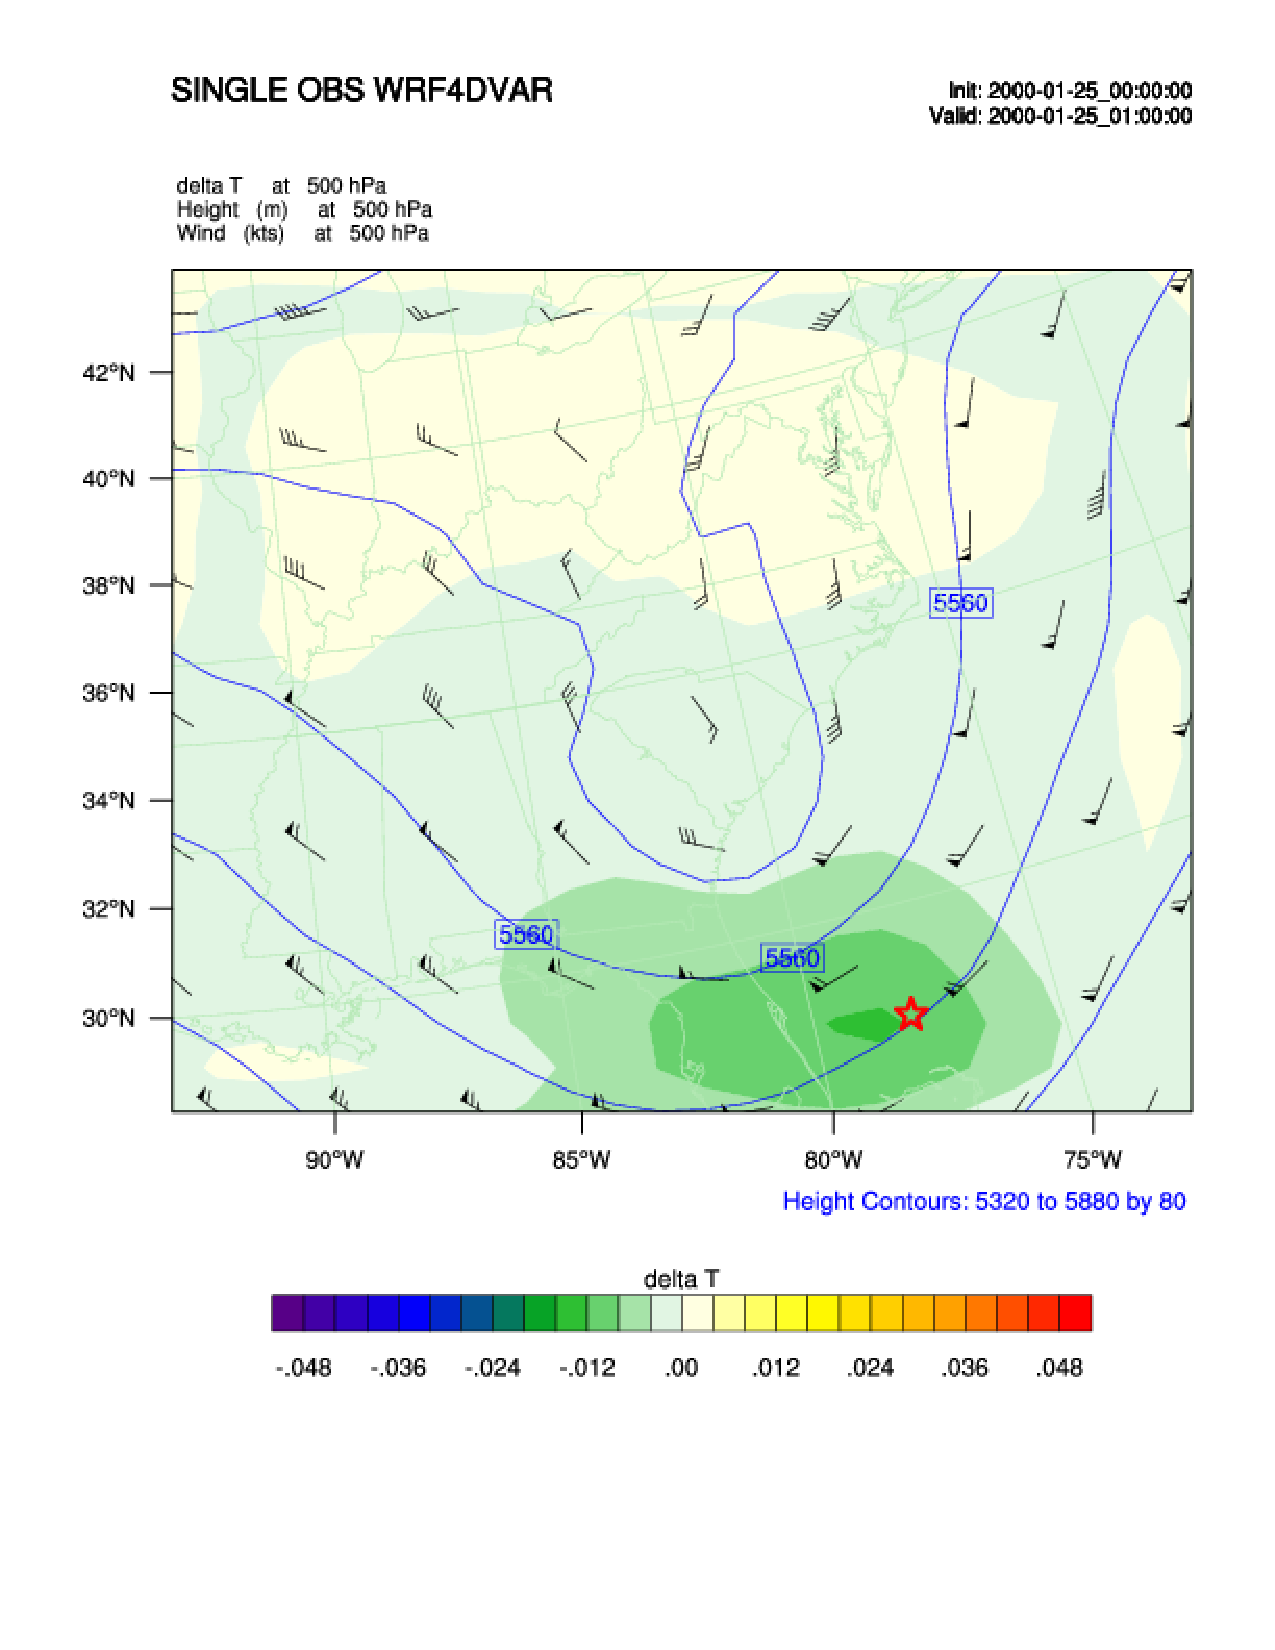
\includegraphics[width=0.6\textwidth]{figures/boundary_1h} 
\end{figure} 
\end{frame}

\begin{frame}
\frametitle{500hPa $\theta$ increments at {\color{red}02h} w/o LBC control}
\begin{figure} 
\centering 
\centering 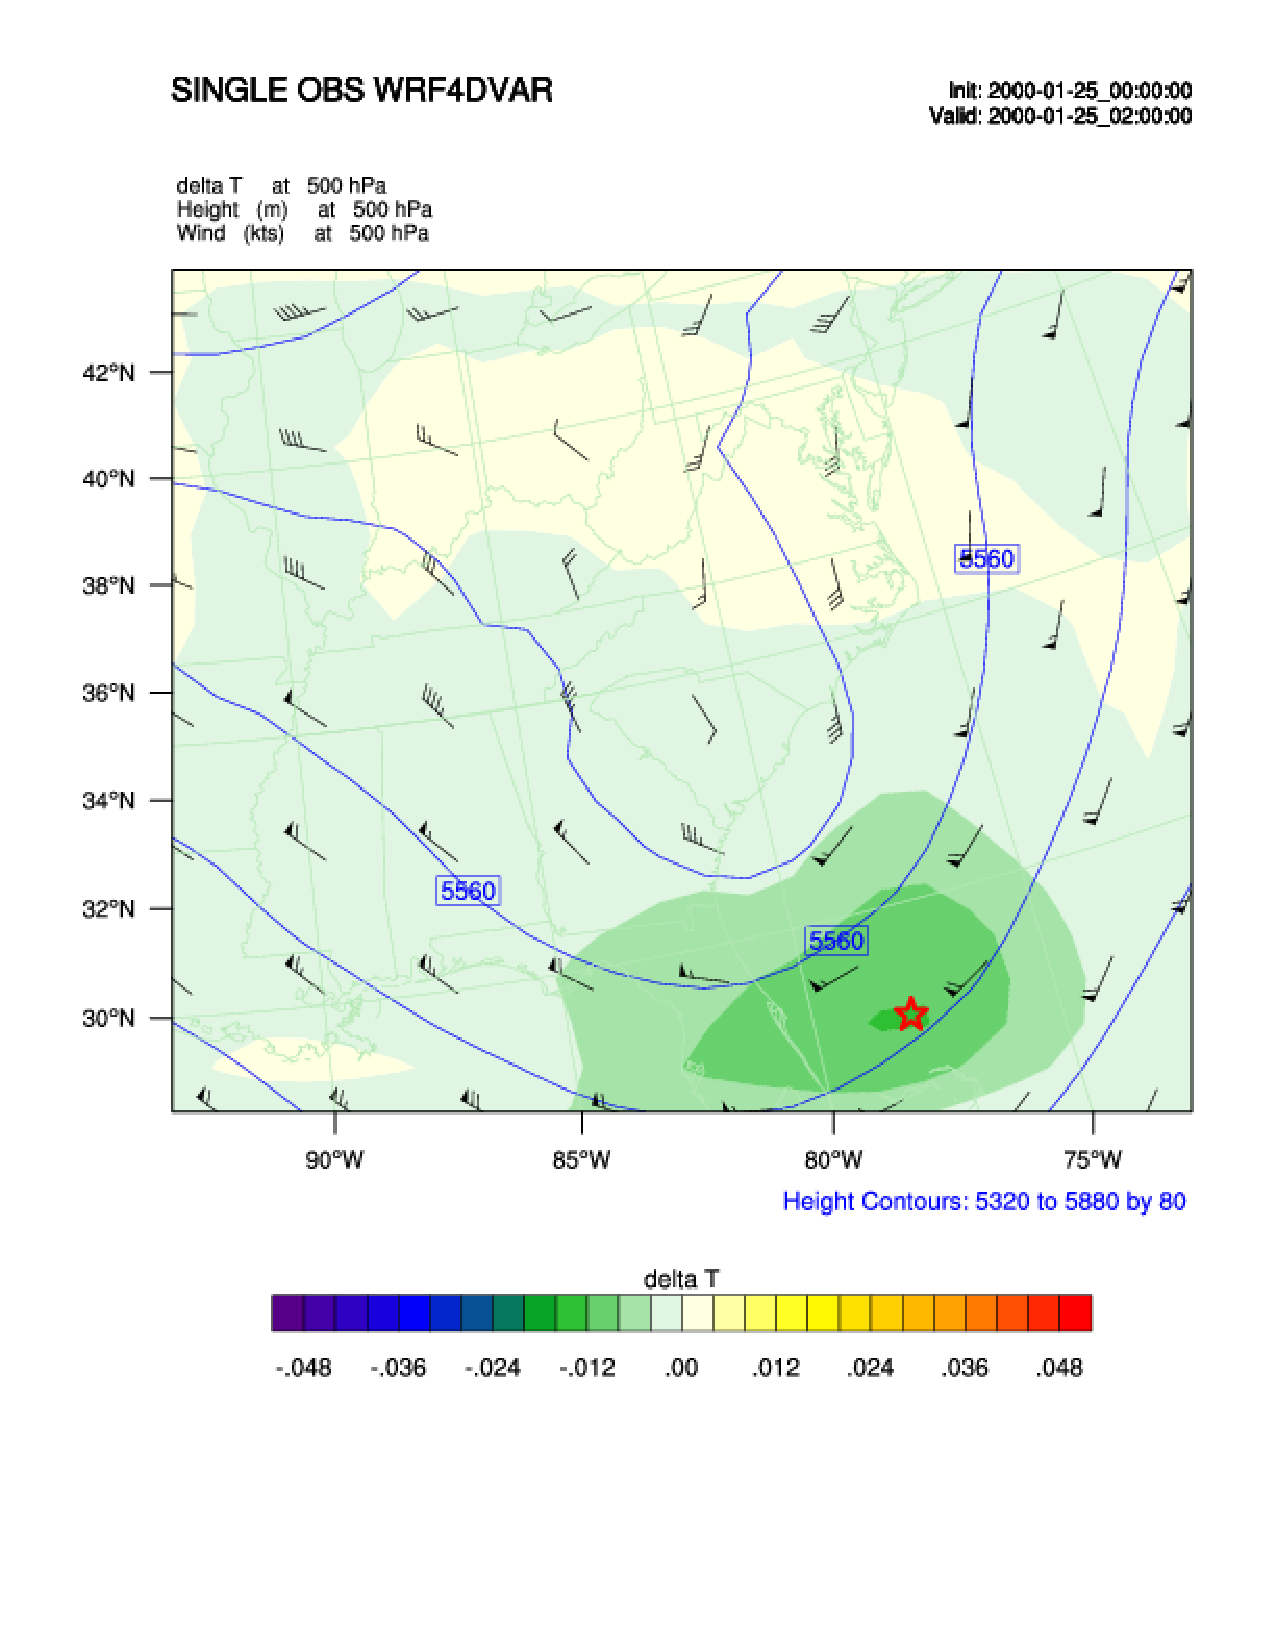
\includegraphics[width=0.6\textwidth]{figures/boundary_2h} 
\end{figure} 
\end{frame}

\begin{frame}
\frametitle{500hPa $\theta$ increments at {\color{red}03h} w/o LBC control}
\begin{figure} 
\centering 
\centering 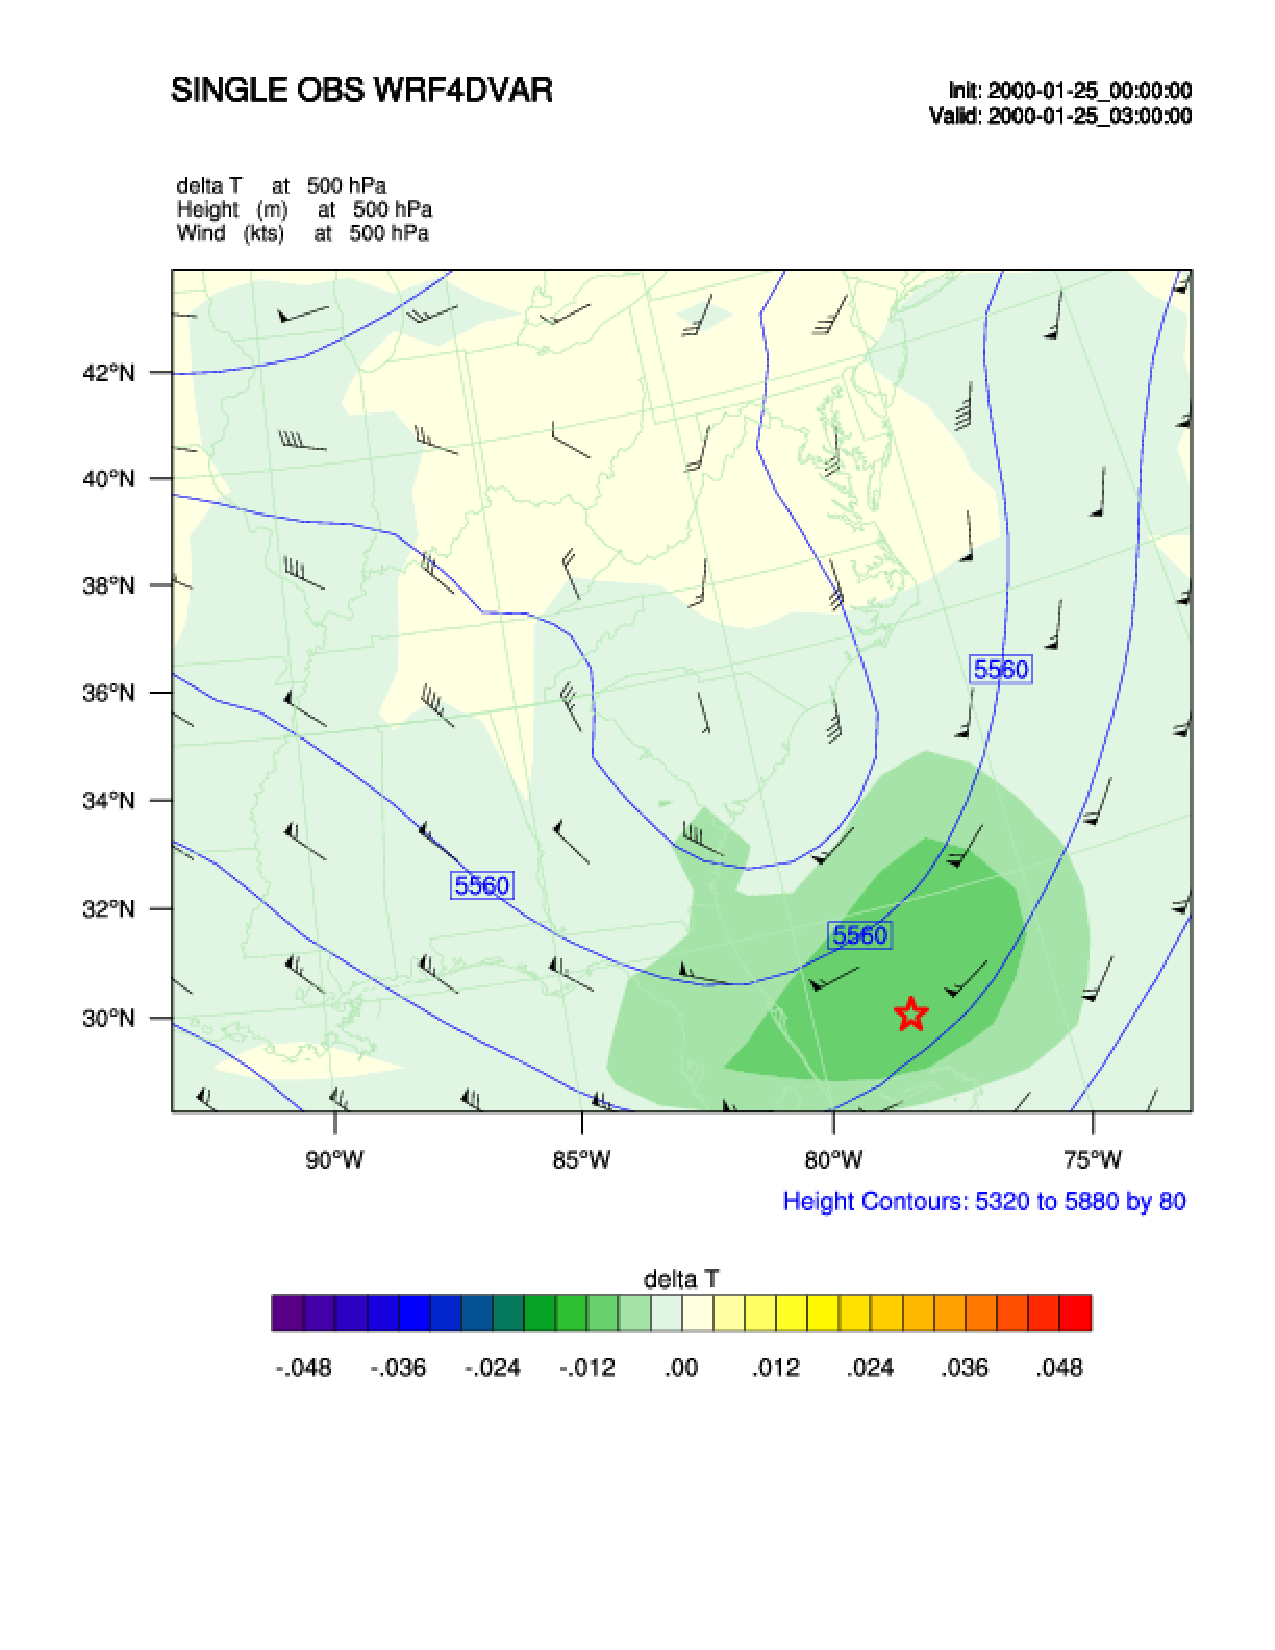
\includegraphics[width=0.6\textwidth]{figures/boundary_3h} 
\end{figure} 
\end{frame}

\begin{frame}
\frametitle{500hPa $\theta$ increments at {\color{red}04h} w/o LBC control}
\begin{figure} 
\centering 
\centering 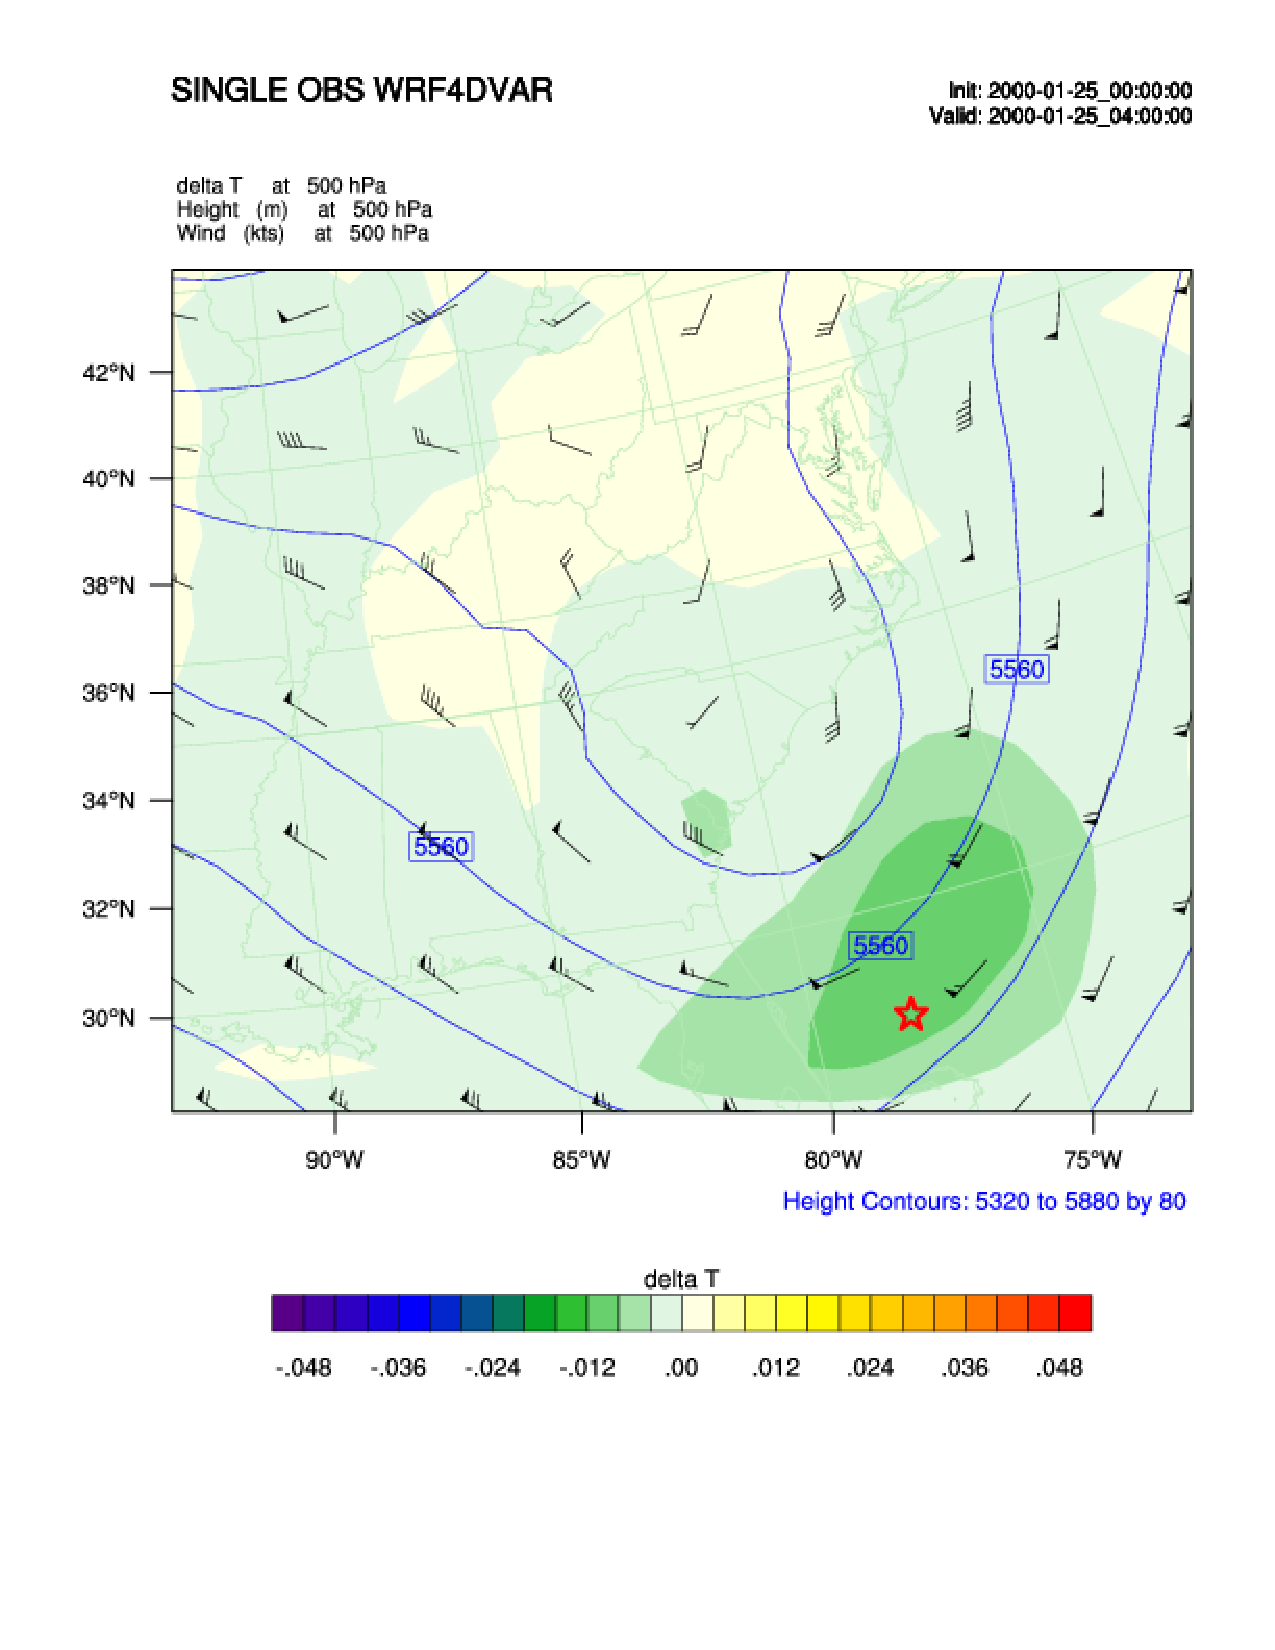
\includegraphics[width=0.6\textwidth]{figures/boundary_4h} 
\end{figure} 
\end{frame}

\begin{frame}
\frametitle{500hPa $\theta$ increments at {\color{red}05h} w/o LBC control}
\begin{figure} 
\centering 
\centering 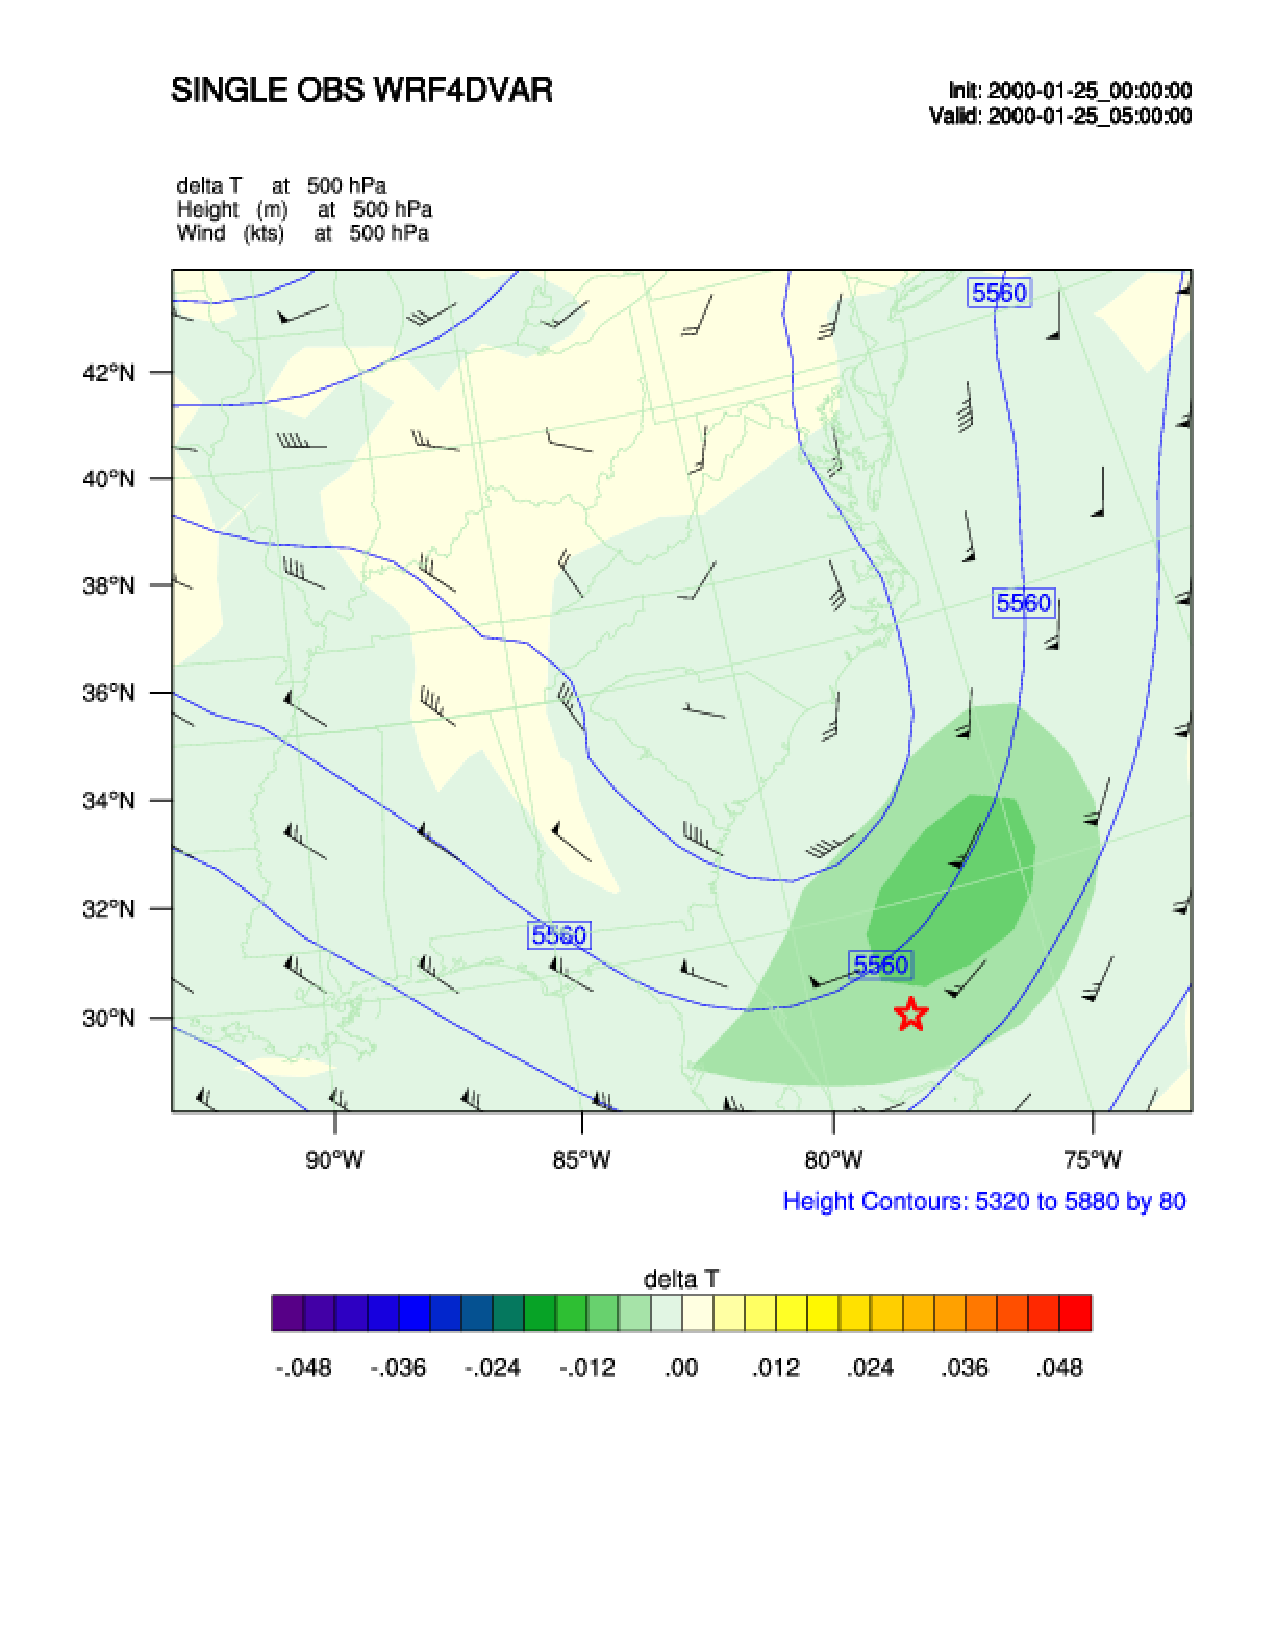
\includegraphics[width=0.6\textwidth]{figures/boundary_5h} 
\end{figure} 
\end{frame}

\begin{frame}
\frametitle{500hPa $\theta$ increments at {\color{red}06h} w/o LBC control}
\begin{figure} 
\centering 
\centering 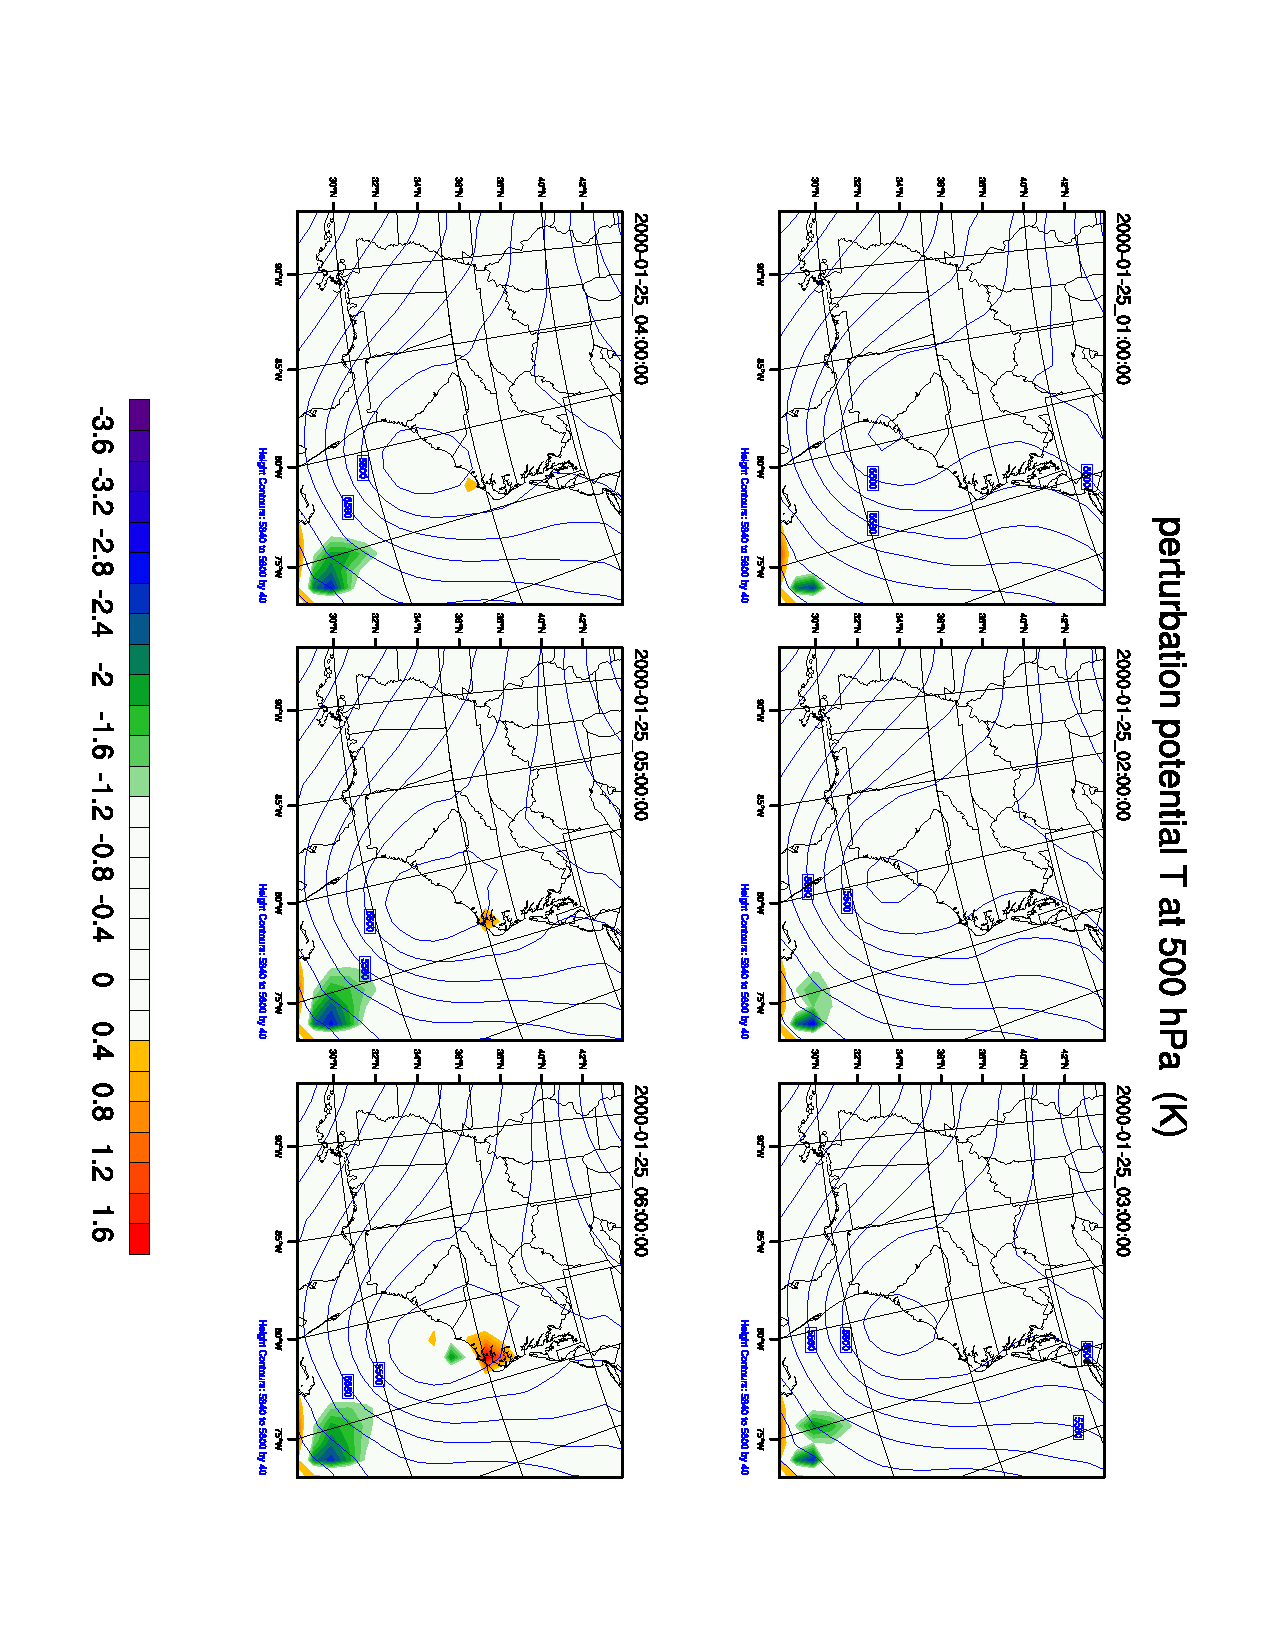
\includegraphics[width=0.6\textwidth]{figures/boundary_6h} 
\end{figure} 
\end{frame}

\begin{frame}
\begin{itemize}
\item Clearly flow-dependent increments is located upstream the observation in IC. \pause
\item Only the boundary conditions at the start of the assimilation window is changed and which at the end of window is kept unchanged \pause
\item The analysis increment of -0.04K at the observation location on 6h. \pause
\item The main analysis increments pass away the observation on 6h
\end{itemize}
\end{frame}

\section{Summary}

\begin{frame}
\frametitle{Summary and Discussion}
\begin{itemize}
\item Single observation experiments confirm the implementation of  LBC control in WRF 4D-Var \pause
\item Inclusion of LBC control in 4D-Var helps to obtain an analysis which fits the observation better \pause
\item The preliminary real observation experiments with LBC control don't show noticeable improvement, but Gustafsson (personal communication) implemented LBC control with same way in the HIRLAM 4D-Var system and the one-month operational experiment show the positive impact on verification score.
\end{itemize}
\end{frame}

\begin{frame}
\frametitle{Summary and Discussion}
\begin{itemize}
\item A common question regarding to the correlation between control variables at the start and the end of the window, Gustafsson (personal communication) confirmed that the correlation is very small in HIRLAM , which means the 4D-Var with LBC should be well conditioned. \pause
\item Our experiments with LBC control don't show more iterations are needed to converge compared to those without LBC control .
\end{itemize}
\end{frame}

\end{document}
